\PassOptionsToPackage{table, dvipsnames}{xcolor}
\documentclass[a4paper,oneside,12pt]{report}

\usepackage[a4paper,margin=3cm]{geometry}
\usepackage[T1]{fontenc}
\usepackage{lmodern}
\usepackage[utf8]{inputenc}
\usepackage[italian]{babel}
\usepackage{float}
\usepackage{graphicx}
\usepackage{svg}
\usepackage{tikz}
\usepackage{amsmath}
\usetikzlibrary{positioning}
\usepackage{booktabs}
\usepackage{longtable}
\usepackage{array}
\usepackage{enumitem}
\usepackage{xurl}
\usepackage{longtable}
\usepackage{booktabs}
\usepackage{array}
\usepackage{xcolor}
\usepackage{listings}

\definecolor{yamlBlue}{RGB}{0,70,140}
\definecolor{yamlGreen}{RGB}{0,120,80}
\definecolor{yamlGray}{RGB}{90,90,90}
\definecolor{yamlPurple}{RGB}{120,60,150}
\definecolor{codeBg}{RGB}{248,248,248}

\lstdefinelanguage{yaml}{
  keywords={true,false,null,y,n,yes,no,on,off},
  keywordstyle=\color{yamlPurple}\bfseries,
  basicstyle=\ttfamily\scriptsize,
  sensitive=false,
  comment=[l]{\#},
  commentstyle=\color{yamlGray}\itshape,
  morestring=[b]',
  morestring=[b]",
  stringstyle=\color{yamlGreen},
  literate=
    {0}{{{\color{yamlPurple}0}}}1
    {1}{{{\color{yamlPurple}1}}}1
    {2}{{{\color{yamlPurple}2}}}1
    {3}{{{\color{yamlPurple}3}}}1
    {4}{{{\color{yamlPurple}4}}}1
    {5}{{{\color{yamlPurple}5}}}1
    {6}{{{\color{yamlPurple}6}}}1
    {7}{{{\color{yamlPurple}7}}}1
    {8}{{{\color{yamlPurple}8}}}1
    {9}{{{\color{yamlPurple}9}}}1
    {:}{{{\color{yamlBlue}:}}}1
    {-}{{{\color{yamlBlue}-}}}1
}

\lstset{
    language=yaml,
    backgroundcolor=\color{codeBg},
    basicstyle=\ttfamily\scriptsize,
    breaklines=true,
    breakatwhitespace=false,
    columns=fullflexible,
    keepspaces=true,
    showstringspaces=false,
    frame=single,
    rulecolor=\color{yamlGray},
    tabsize=2,
    captionpos=b,
    numbers=left,
    numberstyle=\tiny\color{yamlGray},
    numbersep=8pt
}

\usepackage[newfloat]{minted}
\SetupFloatingEnvironment{listing}{name=Codice}
\usepackage[font=small,skip=1pt]{caption}

\usepackage{hyperref}
\hypersetup{colorlinks=true,allcolors=black,pageanchor=false}

\pdfsuppresswarningpagegroup=1
\setlength{\emergencystretch}{3em}
\hbadness=10000
\newcommand{\apiendpoint}[1]{\path{#1}}

\setlist[itemize]{itemsep=2pt, topsep=4pt}
\setlength{\parskip}{0.35em}
\setlength{\parindent}{0pt}
\renewcommand{\arraystretch}{1.25}

\begin{document}
\frenchspacing

\pagenumbering{gobble}

\newcommand{\institutionName}{POLITECNICO DI BARI | TP}
\newcommand{\projectWorkType}{Project work}
\newcommand{\courseName}{Modelli di E-Business e Business Intelligence/Digital Business}
\newcommand{\documentType}{Relazione finale}

\newcommand{\projectTitleLineOne}{Chatbot AI multimodale per customer care}
\newcommand{\projectTitleLineTwo}{Giochi del Mediterraneo Taranto 2026}

\newcommand{\studentsLabel}{Studenti}
\newcommand{\studentsNames}{
Roberto Carriero\par
Ivano Di Ceglie\par
Giuseppe Fuscaldi\par
Angelo Mastrangelo
}

\newcommand{\professorLabel}{Docente}
\newcommand{\professorName}{Prof.\ Umberto Panniello}

\newcommand{\companyTutorsLabel}{Tutor aziendali}
\newcommand{\companyTutorsNames}{
Eugenio Fumarola\par
Domenico Zurlo
}

\newcommand{\academicYearLabel}{Anno accademico 2025/2026}

\begin{titlepage}
\thispagestyle{empty}

\begin{center}

    \vspace*{0.35cm}

    \makebox[\textwidth][c]{
        
\includegraphics[height=3.45cm,keepaspectratio]{images/logo.png}
        \hspace{0.35cm}
        
\includegraphics[height=3.45cm,keepaspectratio]{images/logo_tp.jpg}
    }

    \vspace{0.55cm}

    {\Large\bfseries \institutionName\par}

    \vspace{0.95cm}

    {\large\bfseries \projectWorkType\par}

    \vspace{0.22cm}

    {\large \courseName\par}

    \vspace{1.4cm}

    {\large\bfseries \documentType\par}

    \vspace{0.5cm}

    \makebox[\textwidth][c]{
        \begin{minipage}{1.25\textwidth}
            \centering
            {\bfseries\fontsize{22pt}{30pt}\selectfont
            \projectTitleLineOne:\par
            \projectTitleLineTwo\par}
        \end{minipage}
    }

    \vfill

    \begin{minipage}[t]{0.45\textwidth}
        \raggedright{}

        {\large\bfseries \professorLabel\par}
        \vspace{0.15cm}
        {\large \professorName\par}

        \vspace{0.85cm}

        {\large\bfseries \companyTutorsLabel\par}
        \vspace{0.15cm}
        {\large \companyTutorsNames\par}
    \end{minipage}
    \hfill
    \begin{minipage}[t]{0.45\textwidth}
        \raggedleft{}

        {\large\bfseries \studentsLabel\par}
        \vspace{0.15cm}
        {\large \studentsNames\par}
    \end{minipage}

    \vfill

    {\large \academicYearLabel\par}

    \vspace*{0.45cm}

\end{center}

\end{titlepage}

\chapter*{Abstract}

La presente relazione descrive il project work sviluppato in collaborazione con TP, avente come oggetto la progettazione e la realizzazione di T.A.L.O.S. \textit{(Taranto 2026 AI Live Operator Support)}, una soluzione basata su intelligenza artificiale multimodale per il supporto al customer care dei Giochi del Mediterraneo 2026 a Taranto.

Il progetto prende avvio da una precisa esigenza operativa: superare la frammentazione delle fonti informative che caratterizza gli eventi internazionali, garantendo così un flusso di dati e di informazioni coerente e accessibile. In un contesto caratterizzato da cittadini, turisti e stakeholder provenienti da Paesi differenti, la disponibilità di un canale informativo unico rappresenta un elemento decisivo per migliorare l’esperienza dell’utente e ridurre il carico sui canali tradizionali di assistenza.

T.A.L.O.S. è stato quindi progettato come un sistema completo, in grado di supportare l’utente secondo le sue esigenze al fine di rendere la sua esperienza quanto più soddisfacente possibile. La soluzione integra un’interfaccia responsive, consultabile da qualsiasi dispositivo, attraverso cui l’utente può accedere a un chatbot basato su una pipeline di \textit{Retrieval-Augmented Generation} (RAG) applicata a una base di conoscenza specifica per il contesto dei Giochi del Mediterraneo 2026. Il sistema supporta inoltre la multimodalità, consentendo l’invio di richieste in formato testuale, vocale e visuale, che vengono elaborate e ricondotte a una rappresentazione comune per generare risposte testuali multilingua in linguaggio naturale.

Quando una richiesta non può essere gestita in modo affidabile in autonomia, oppure quando l’utente esprime insoddisfazione rispetto alla risposta ricevuta, il sistema consente l’apertura di un ticket verso un operatore di customer care. L’operatore dispone di una dashboard riservata per consultare i ticket, visualizzare il contesto della conversazione e gestire la richiesta. È inoltre presente una pagina dedicata all'organizzazione della knowledge base, attraverso cui è possibile inserire nuovi contenuti informativi tramite interfaccia grafica alla portata di tutti, indipendentemente dal livello di competenza tecnica.

Infine, il progetto include un flusso di testing automatizzato basato su un dataset di casi simulati, costruiti per rappresentare possibili interazioni utente. La valutazione misura diverse metriche quantitative relative a diversi aspetti del sistema, riconducibili a specifici \textit{Key Performance Indicator} (KPI).
\tableofcontents

\cleardoublepage{}
\pagenumbering{arabic}
\setcounter{page}{1}

\chapter{Introduzione}

\section{Contesto}

I Giochi del Mediterraneo 2026 a Taranto rappresentano un evento sportivo internazionale di ampia portata, con il coinvolgimento di numerosi atleti, discipline, impianti e città. In un contesto di questo tipo, la gestione delle informazioni diventa un aspetto critico, in quanto gli utenti possono riscontrare difficoltà nel reperire risposte chiare, coerenti e univoche rispetto alle proprie esigenze.

La criticità principale è la frammentazione informativa. Le fonti disponibili risultano spesso distribuite tra siti web, documenti e canali differenti. Questo rende il recupero delle informazioni meno immediato e semplice per l’utente finale, che potrebbe essere indotto a contattare referenti o esperti del settore, incrementando così il carico di richieste da gestire manualmente.

Pertanto, nella presente relazione viene presentata una soluzione innovativa sviluppata in collaborazione con TP, che mette in relazione le esigenze degli utenti interessati ai Giochi con una gestione efficiente del customer care. Il progetto sfrutta le potenzialità dell’intelligenza artificiale, misurate attraverso metriche quantitative e specifici \textit{Key Performance Indicator} (KPI).

\section{Obiettivi}

L’obiettivo principale del progetto è realizzare un chatbot AI multimodale per il contesto presentato in precedenza. Il sistema deve essere accessibile e utilizzabile da qualsiasi dispositivo e deve fornire risposte in linguaggio naturale basate sulle informazioni presenti nell’apposita base di conoscenza mediante \textit{Retrieval-Augmented Generation} (RAG). La multimodalità consente all'utente di interagire con il chatbot secondo le proprie esigenze, garantendo una risposta adeguata indipendentemente dalla struttura dell'input.

Un aspetto fondamentale riguarda l’integrazione del chatbot nel processo operativo di assistenza. Quando la risposta automatica non è sufficiente o non soddisfa l’utente, il sistema deve consentire l’apertura di un ticket verso un operatore umano, conservando il contesto utile affinché l'operatore sia in grado di rispondere in modo informato ed esaustivo.

Nello specifico, il sistema comprende una chat multilingua con interfaccia disponibile in italiano, inglese, spagnolo, francese e arabo, ovvero le lingue principali parlate nei paesi che si affacciano sul Mar Mediterraneo. La chat consente lo scambio di messaggi tra utente e bot e permette all’utente di valutare la risposta ricevuta mediante un feedback in grado di orientare le successive fasi di gestione del ticket. Ogni interazione viene salvata in una base di dati, così da rendere possibile l’analisi dei flussi conversazionali e la generazione di valore tramite attività di \textit{data mining} e \textit{business intelligence}.

Il progetto include anche una dashboard operatore ad accesso riservato. Attraverso questa pagina, l’operatore può gestire i ticket, visualizzare le conversazioni, tradurle e ottenere suggerimenti utili per l’e-mail di risposta.

Infine, è presente un’ulteriore pagina dedicata alla gestione della base di conoscenza. Questa funzionalità consente di aggiornare nel tempo i contenuti informativi del sistema tramite un’interfaccia grafica realizzata appositamente per profili non tecnici. Tale scelta si adatta bene al contesto applicativo, poiché gli eventi sportivi sono dinamici e le informazioni possono essere integrate o aggiornate progressivamente.

\section{Valore strategico}

Dal punto di vista aziendale, il valore della soluzione deriva dalla possibilità di ridurre l’intervento umano nelle richieste informative di primo livello. Il chatbot consente infatti di soddisfare automaticamente parte delle domande ricorrenti, lasciando agli operatori umani i casi più complessi o non risolvibili sulla base delle informazioni disponibili. Inoltre, ciò può tradursi in una riduzione dei costi di gestione e in una migliore allocazione del personale, che può essere spostato da attività ripetitive di assistenza verso compiti a maggiore valore aggiunto.

La scelta di ricorrere a un operatore umano quando il sistema non riesce a fornire una risposta automatica affidabile è coerente con la logica \textit{Human-in-the-Loop}. In questo approccio, l’intelligenza artificiale supporta e velocizza la gestione delle richieste più ricorrenti, mentre il consulente mantiene un ruolo centrale nei casi critici.

In ottica di business intelligence, l’analisi successiva di conversazioni, ticket e feedback permette di comprendere quali informazioni siano più richieste dagli utenti e quali aree risultino ancora incomplete nella base di conoscenza. Questi dati aiutano il committente ad ampliare in modo mirato il dominio informativo del sistema, aggiornando i contenuti e anticipando possibili domande future.

Nel modello adottato sono presenti tre attori principali. Il primo è l’utente finale, che può essere un cittadino, un turista o una persona interessata ai Giochi del Mediterraneo, che ha bisogno di ottenere risposte rapide e comprensibili.

Il secondo attore è l’operatore di customer care, per il quale il valore principale del sistema consiste nell’accesso completo al contesto della conversazione. In questo modo, l’operatore può comprendere meglio la richiesta ed evitare domande ripetitive all’utente.

Il terzo attore è l’organizzazione che gestisce il servizio. Per essa, il valore della soluzione risiede nella possibilità di osservare l’andamento delle richieste e migliorare il livello di soddisfazione dell'utente, che se riceve informazioni corrette è più propenso a vivere l’evento in modo positivo, partecipando ad attività gratuite e a pagamento.

Per riassumere il valore generato dal progetto, il \textit{Business Model Canvas} è riportato in Figura~\ref{fig:bmc}.

\begin{figure}[H]
\centering
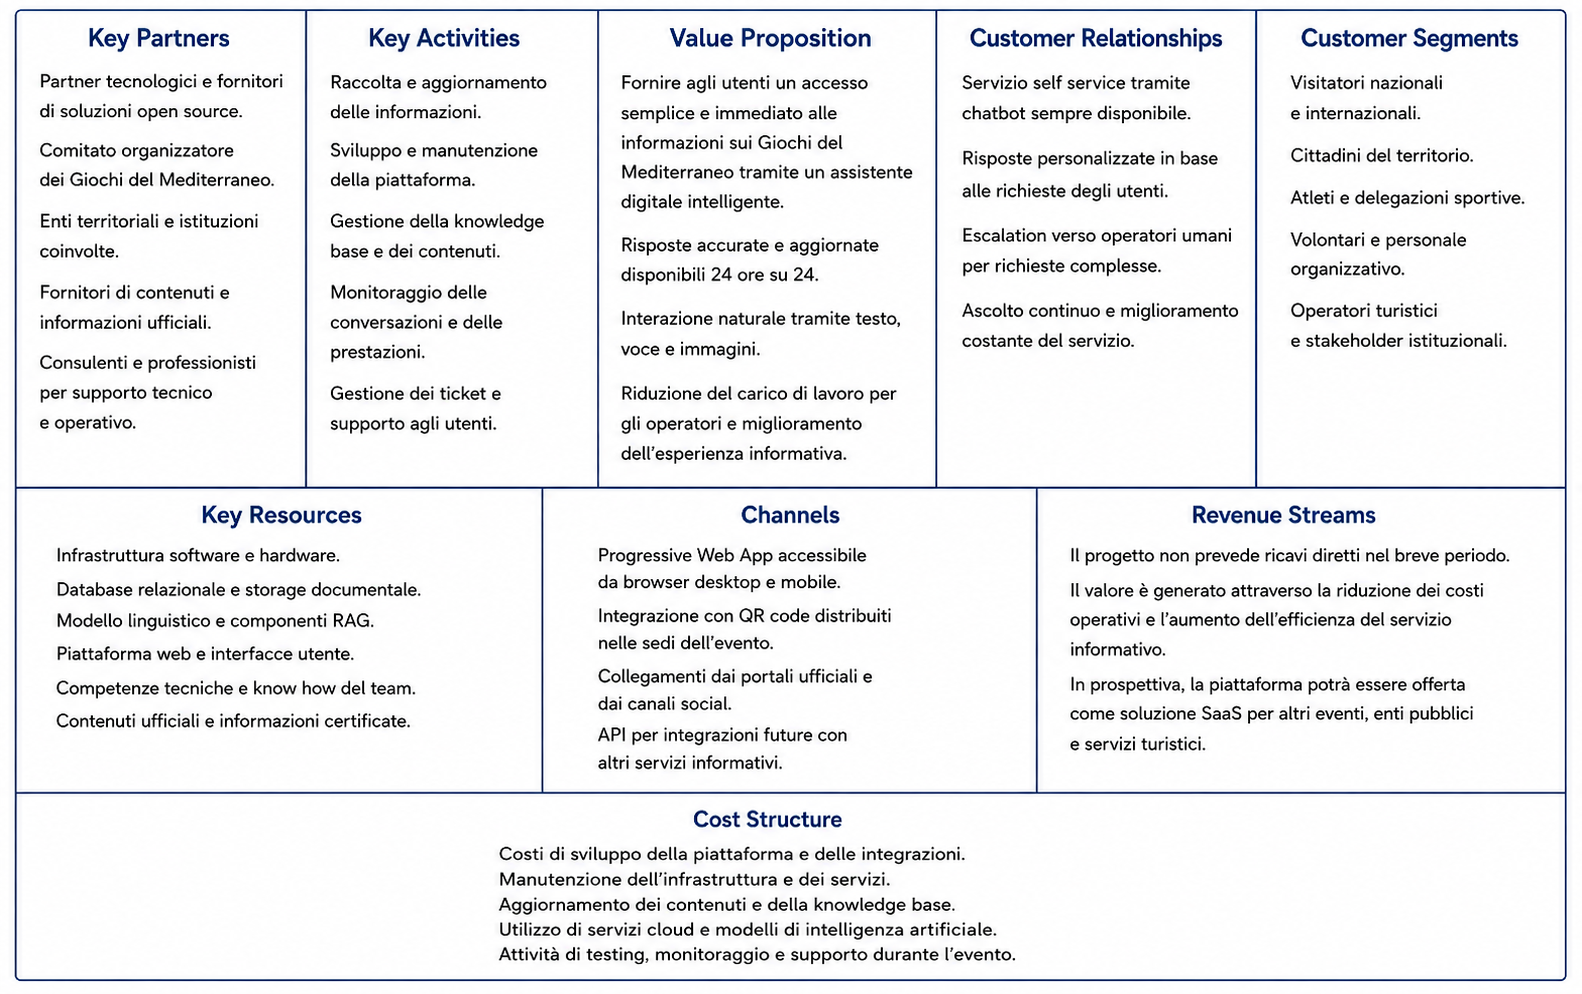
\includegraphics[width=0.98\textwidth]{images/bmc.png}
\caption{Business Model Canvas del progetto.}\label{fig:bmc}
\end{figure}

Nel canvas, la \textit{value proposition} consiste nel fornire agli utenti un accesso semplice e immediato alle informazioni attraverso un assistente intelligente e nella riduzione del carico operativo per gli operatori. Inoltre, la \textit{customer relationship} con gli utenti si basa su un modello di \textit{self-service} assistito, in cui il chatbot è sempre disponibile per le richieste comuni, mentre l’escalation verso l’operatore umano viene prevista per i casi complessi.

Dal punto di vista economico, il progetto non prevede ricavi diretti nel breve periodo, poiché nasce come soluzione di supporto informativo e operativo. Il valore viene generato soprattutto attraverso la riduzione dei costi di assistenza, l’aumento dell’efficienza del servizio e il miglioramento della qualità percepita dagli utenti.

A completamento dell’analisi di business è stata svolta anche un'analisi \textit{Strengths, Weaknesses, Opportunities and Threats} (SWOT), riportata in Figura~\ref{fig:swot}.

\begin{figure}[H]
\centering
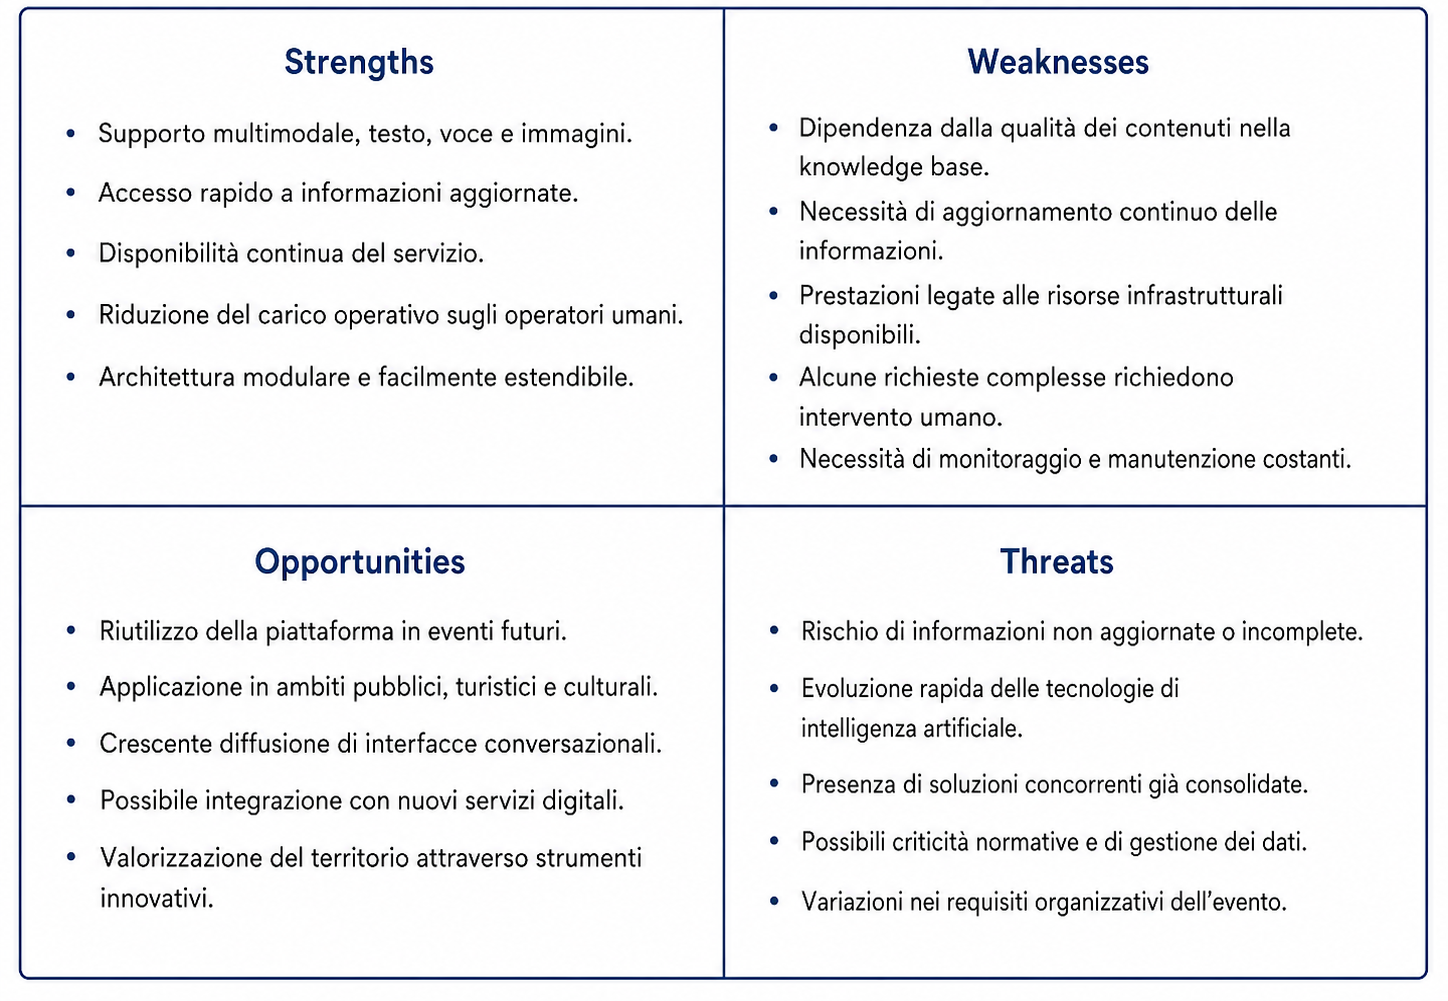
\includegraphics[width=0.98\textwidth]{images/swot.png}
\caption{Analisi SWOT del progetto.}\label{fig:swot}
\end{figure}

Tra i principali punti di forza rientrano il supporto multimodale, la disponibilità continua del servizio e la riduzione del carico operativo sugli operatori.

Le debolezze riguardano soprattutto la dipendenza dalla qualità della \textit{knowledge base} e la necessità di intervento umano in alcuni casi specifici non risolvibili in modo affidabile dal bot.

Le opportunità sono legate alla possibilità di riutilizzare la piattaforma in eventi futuri con le stesse criticità e all’evoluzione dei servizi digitali, sempre più orientati a interazioni naturali e personalizzate.

Le minacce riguardano il rischio di informazioni non aggiornate o incomplete e possibili limitazioni normative.

\section{Stato dell'arte}

Il customer care riguarda l’insieme dei processi attraverso cui un’organizzazione intercetta, comprende e risolve i bisogni degli utenti. In un modello tradizionale, l’utente cerca un’informazione e, se non riesce a trovarla, contatta un operatore umano, al quale deve spesso spiegare nuovamente il problema. Questo approccio può risultare efficace nei casi complessi, ma diventa poco efficiente quando le richieste sono numerose e ripetitive. In un modello digitale intelligente, invece, le richieste ricorrenti vengono rese accessibili in autonomia, mentre l'intervento dell'operatore è riservato ai soli casi che richiedono autonomia decisionale o competenze specialistiche.

Una prima forma di automazione del customer care è rappresentata dai chatbot tradizionali basati su regole. Questi sistemi sono efficaci quando il dominio applicativo è limitato e il flusso conversazionale può essere descritto tramite scelte predefinite, FAQ o alberi decisionali. In molti contesti aziendali possono quindi supportare attività semplici, ma risultano meno adatti in scenari complessi e dinamici.

I modelli linguistici generativi hanno ampliato le possibilità di interazione, poiché sono in grado di comprendere meglio il linguaggio naturale e produrre risposte discorsive. Tuttavia, un modello linguistico generico non possiede necessariamente informazioni aggiornate rispetto alle fonti necessarie e, in assenza di un contesto informativo adeguato, può generare contenuti non verificati. Questo fenomeno, definito allucinazione, comporta un rischio non trascurabile nel customer care: un'informazione errata è spesso più dannosa di una mancata risposta.

Per questo motivo, l’architettura RAG rappresenta una soluzione adatta per domini informativi specifici. La domanda dell’utente viene prima utilizzata per recuperare dalla base di conoscenza i documenti semanticamente più pertinenti e solo successivamente il modello linguistico genera la risposta, utilizzando le fonti recuperate come contesto.

Di seguito, in Tabella \ref{tab:valore-processo-assistenza}, sono riassunte le principali differenze tra customer care tradizionale e soluzioni digitali innovative.

\begin{longtable}{p{0.30\textwidth}p{0.30\textwidth}p{0.30\textwidth}}
\caption{Confronto tra assistenza tradizionale e progetto proposto.}\label{tab:valore-processo-assistenza}\\
\toprule
\textbf{Aspetto} & \textbf{Tradizionale} & \textbf{Automatizzato}\\
\midrule
\textbf{Accesso alle informazioni} & Ricerca manuale tra più fonti. & Punto informativo unico.\\
\textbf{Richieste ripetitive} & Gestite da operatore umano. & Gestite in autonomia quando coperte dalla KB.\\
\textbf{Casi complessi} & Non sempre arrivano strutturati. & Arrivano come ticket con contesto.\\
\textbf{Aggiornamento dei contenuti} & Dipende da modifiche manuali. & Possibile tramite interfaccia guidata e intuitiva.\\
\textbf{Impatto} & Limitata a valutazione di statistiche generiche. & Valutato tramite KPI su qualità informativa, tecnica e operativa.\\
\bottomrule
\end{longtable}
\chapter{Analisi preliminare}

Nel presente capitolo viene descritta l’analisi preliminare svolta a monte dello sviluppo del sistema. Essa ha riguardato la definizione del problema, l’individuazione degli obiettivi e la suddivisione di ruoli e attività tra i membri del gruppo.

\section{Ruoli e gestione del gruppo}

Il team di progetto è eterogeneo ed è composto da quattro studenti, due provenienti da Ingegneria Informatica e due da Ingegneria Gestionale. In generale, la separazione dei ruoli non è stata vincolante, ma ha favorito la collaborazione continua tra i due team mediante contaminazioni costruttive.

I membri di area gestionale si sono occupati principalmente della pianificazione temporale del progetto, articolando le macro-attività e le relative sotto-attività attraverso un diagramma di Gantt. Tale fase è stata supportata da una \textit{Work Breakdown Structure} (WBS), utilizzata per scomporre il progetto in fasi dettagliate e sequenziali, organizzando le attività in modo progressivo.

Gli studenti di area informatica si sono invece occupati della progettazione e dello sviluppo del sistema. In particolare, il lavoro ha riguardato l’analisi dei requisiti funzionali e non funzionali, il \textit{benchmarking} tecnologico, la progettazione dell’architettura, l’implementazione di tutti i moduli software e la fase finale di test e deployment del prototipo.

Nella prima fase, il team gestionale ha partecipato al recupero delle informazioni dalle fonti ufficiali dei Giochi del Mediterraneo e da fonti terze online per la costruzione della knowledge base. Successivamente, il lavoro sui dati è proseguito con la pulizia e il preprocessing dei contenuti testuali fino alla conversione in record strutturati in formato \textit{JSONL}.

In seguito, il team informatico ha svolto la fase di benchmarking tecnologico mediante un'analisi comparativa di diverse soluzioni open-source e commerciali per il retrieval semantico, la generazione di testo e l'integrazione con modelli linguistici di grandi dimensioni (LLM) con l'obiettivo di individuare il compromesso ottimale tra performance, flessibilità e sostenibilità economica per la scelta delle tecnologie da adottare nel progetto. Il team gestionale ha contribuito a tale fase, supportando la valutazione dal punto di vista della compatibilità con gli obiettivi del progetto, dei costi e della coerenza con il valore di business della soluzione.

Nell’ultima fase di test, il lavoro sinergico tra il team gestionale e il team informatico ha permesso di ottenere risultati concreti e misurabili per la valutazione complessiva del sistema. Il team gestionale ha contribuito alla costruzione di un dataset di test il più possibile vicino a potenziali interazioni reali degli utenti, mentre il team informatico ha sviluppato lo script di automazione necessario per eseguire i test e raccogliere le metriche di valutazione.

Trasversalmente a tutte le fasi di progetto, il team gestionale ha avuto il compito di organizzare le riunioni settimanali con i tutor aziendali e di monitorare l’avanzamento rispetto alle scadenze previste nel Gantt, mentre il team informatico ha prodotto i deliverables tecnici e le presentazioni per le riunioni intermedie.

Per la gestione delle attività è stato utilizzato Trello come bacheca principale, secondo un'organizzazione Agile semplificata con \textit{Kanban board}. L'adozione di un approccio Kanban si è rivelata particolarmente efficace per la gestione di un progetto dalla durata contenuta, consentendo al team di mantenere alta la visibilità sullo stato di avanzamento, di identificare tempestivamente eventuali blocchi e di ripianificare le priorità in modo dinamico, senza gli overhead tipici di metodologie più rigorose come Scrum. In Figura~\ref{fig:trello-board} è riportata una schermata della bacheca.

\begin{figure}[H]
\centering
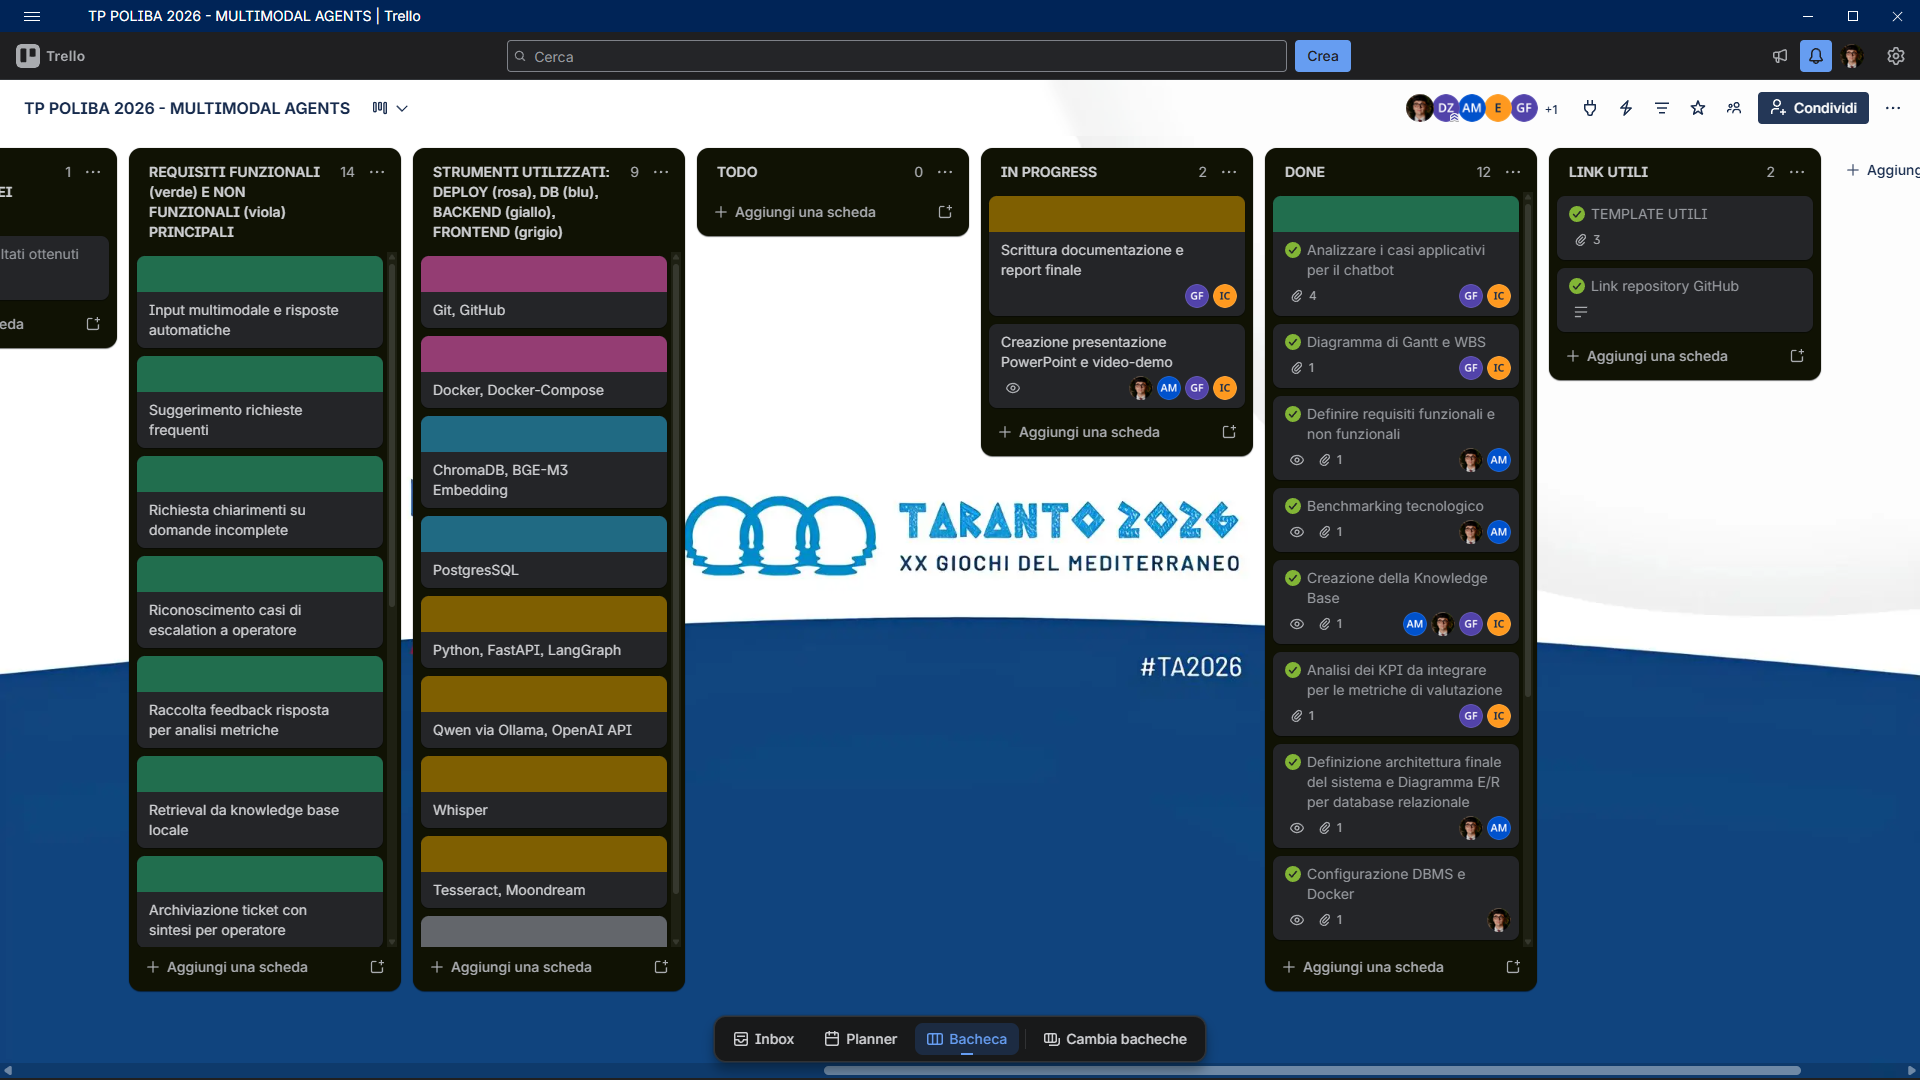
\includegraphics[width=0.95\textwidth]{images/trello-screen.png}
\caption{Bacheca Trello utilizzata per l’organizzazione delle attività di progetto.}\label{fig:trello-board}
\end{figure}

Inoltre, come canali di comunicazione sono stati utilizzati Slack e Microsoft Teams. Il primo ha rappresentato il mezzo principale per interfacciarsi con i tutor aziendali, mentre il secondo è stato utilizzato per le riunioni da remoto e per lo scambio di messaggi e materiale tra i componenti del team. Le principali sfide incontrate hanno riguardato l'integrazione tra le due componenti del team, sia in termini di allineamento terminologico (linguaggio tecnico vs manageriale), sia nella definizione di interfacce chiare tra il lavoro di preparazione dei dati e quello di sviluppo software. Tali difficoltà sono state, però, superate attraverso le riunioni di allineamento frequenti e la creazione di artefatti condivisi (documenti di specifica, dizionario dei dati, repository comune), rafforzando la coesione del gruppo e la qualità complessiva del risultato finale.

\section{Diagramma di Gantt e Work Breakdown Structure}

Il diagramma di Gantt ha avuto lo scopo di distribuire le attività nel tempo e tra le risorse. La WBS, invece, ha permesso di scomporre il progetto in fasi e sotto-attività. Il periodo di lavoro è stato organizzato su un intervallo di circa due mesi, mentre la pianificazione è stata articolata in settimane. Il Gantt sintetico, mostrato in Figura~\ref{fig:gantt-sintesi}, riassume le principali macro-attività svolte dal team, mentre il Gantt dettagliato, mostrato in Figura~\ref{fig:gantt-dettaglio}, esplicita anche le singole sotto-attività, i responsabili e le risorse di supporto.

\begin{figure}[H]
\centering
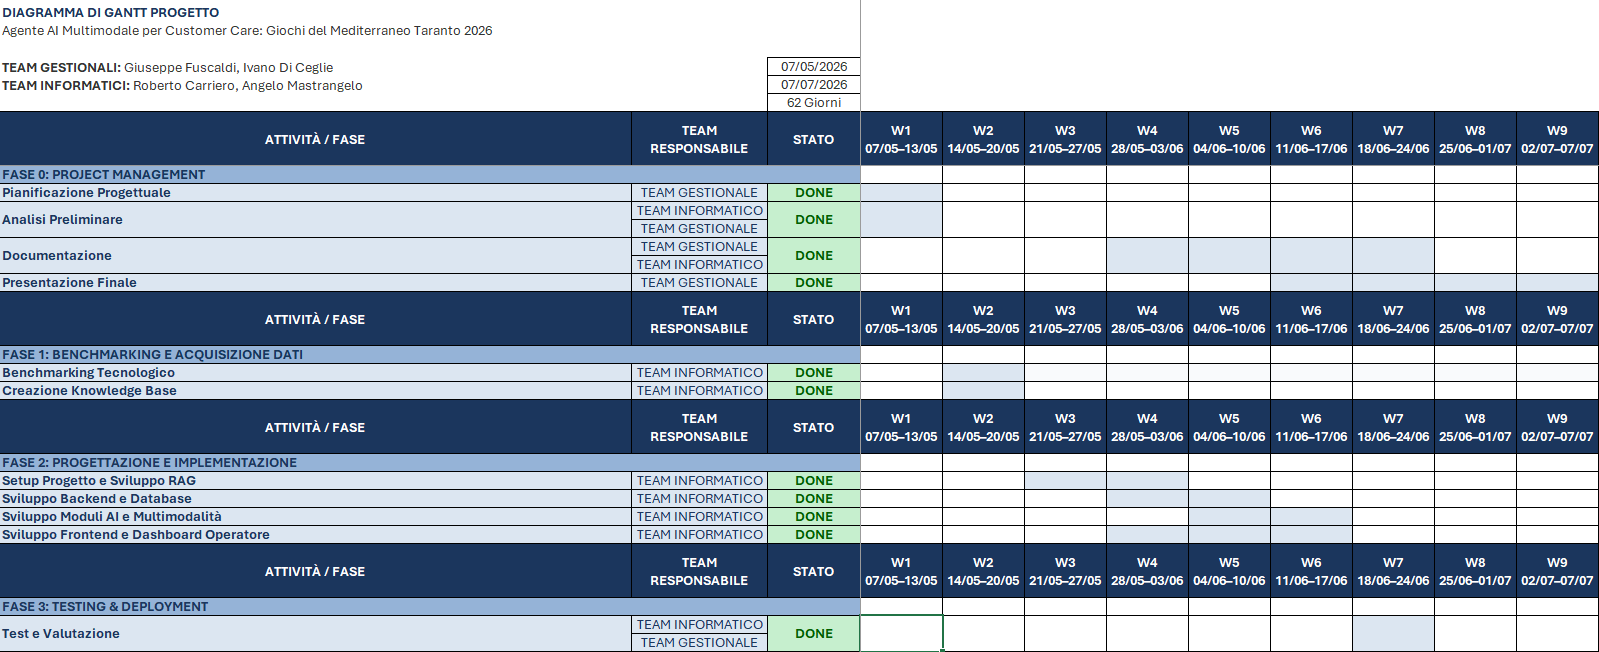
\includegraphics[width=0.95\textwidth]{images/gantt-sintesi.png}
\caption{Rappresentazione sintetica del diagramma di Gantt del progetto.}\label{fig:gantt-sintesi}
\end{figure}

\begin{figure}[H]
\centering
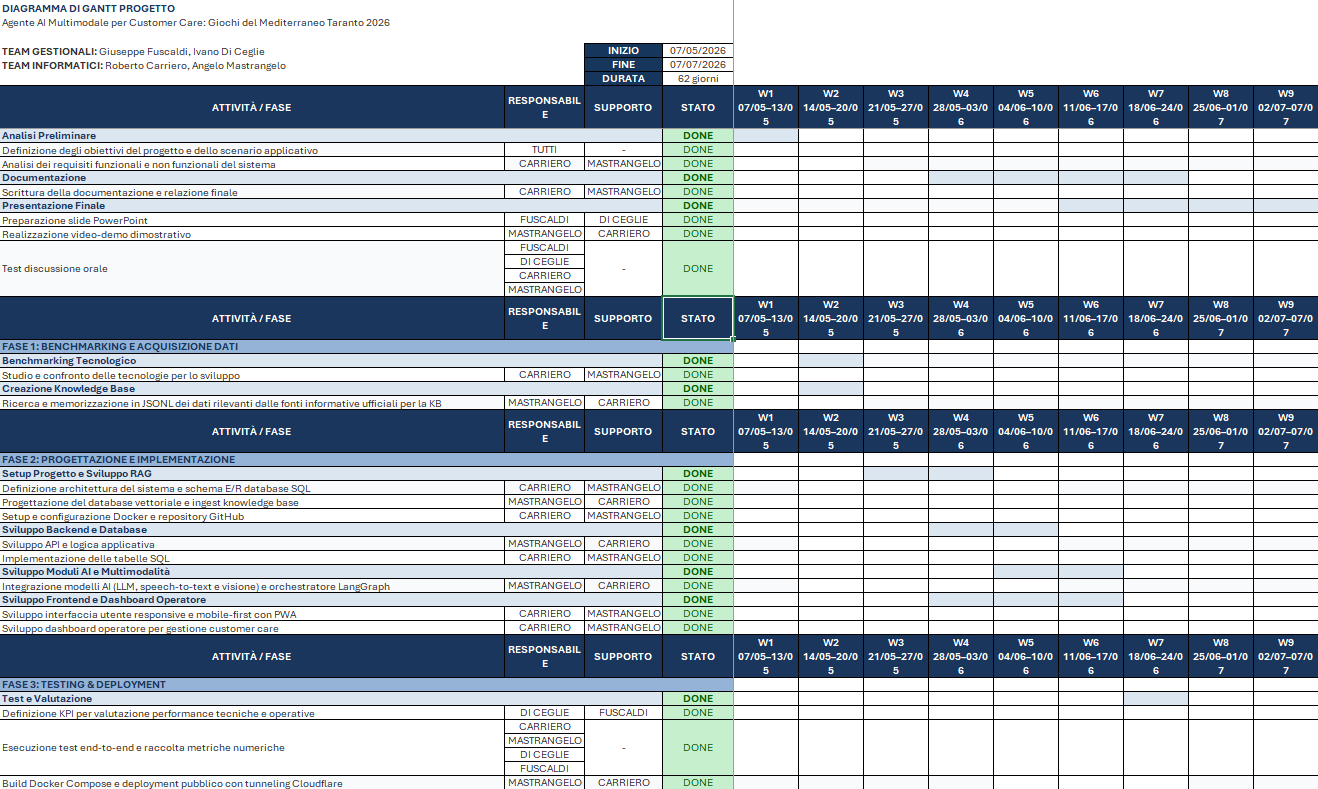
\includegraphics[width=0.95\textwidth]{images/gantt-dettagli.png}
\caption{Rappresentazione dettagliata del diagramma di Gantt con attività, responsabili e avanzamento.}\label{fig:gantt-dettaglio}
\end{figure}

Dal punto di vista organizzativo, il progetto è stato suddiviso in quattro aree. La prima area riguarda il project management e le attività trasversali, la seconda area include il benchmarking e l’acquisizione dei dati, la terza area comprende la progettazione e l’implementazione del sistema, mentre la quarta area integra il testing e il deployment del sistema.

\section{Requisiti funzionali e non funzionali}

La definizione dei requisiti ha anticipato la progettazione del sistema. In generale, per lo sviluppo di una soluzione software è necessario chiarire quali funzionalità essa deve offrire e quali qualità deve garantire.

I requisiti funzionali descrivono le caratteristiche del sistema. Nel caso specifico, il chatbot deve consentire all’utente di formulare richieste in linguaggio naturale e di interagire attraverso formati di input diversi. Tali input devono essere ricondotti a una rappresentazione interna coerente, così da poter essere elaborati dalla stessa pipeline applicativa. Il sistema deve poi recuperare le informazioni rilevanti dalla base di conoscenza, generare risposte automatiche coerenti e aiutare l’utente nell’escalation in caso di insoddisfazione.

Il sistema deve inoltre memorizzare conversazioni, messaggi, feedback e ticket in una base di dati per poterli analizzare successivamente. La raccolta dei feedback è prioritaria, in quanto consente di valutare la qualità percepita della risposta e la soddisfazione dell'utente, mentre la dashboard di customer care rappresenta il principale punto di contatto tra l'utente e l'operatore umano.

Accanto ai requisiti funzionali sono stati definiti i requisiti non funzionali, letti secondo il modello \textit{Functionality, Usability, Reliability, Performance, Supportability +} (FURPS+), come descritto di seguito.

Dal punto di vista della funzionalità \textit{(F)}, il sistema deve interpretare correttamente le richieste, distinguere tra risposta automatica ed escalation e ridurre il rischio di risposte non supportate da fonti certe.
Dal punto di vista dell’usabilità \textit{(U)}, l’interfaccia deve essere semplice e accessibile da diversi dispositivi. Per l’affidabilità \textit{(R)}, il chatbot deve poter gestire input incompleti o poco chiari, privilegiando il chiarimento o il passaggio all’operatore invece di generare informazioni non verificate.
In riferimento alle prestazioni \textit{(P)}, il sistema deve mantenere tempi di risposta compatibili con una conversazione umana, nonostante la complessità della pipeline.
Dal punto di vista della supportabilità \textit{(S)}, l’architettura deve essere modulare, testabile e scalabile. La base di conoscenza deve poter essere aggiornata senza riprogettare il sistema, mentre la containerizzazione deve rendere l’ambiente replicabile su macchine diverse.
Un requisito trasversale è la tracciabilità \textit{(+)}, poiché ogni risposta deve riportare esplicitamente le fonti consultate per garantire l'attendibilità delle risposte automatiche.

\section{Denominazione e branding}

Per il nome del sistema è stato scelto l’acronimo T.A.L.O.S. \textit{(Taranto 2026 AI Live Operator Support)}. Il nome richiama Talos, figura della mitologia greca descritta come un gigante di bronzo creato da Efesto per proteggere l’isola di Creta. Questo riferimento si sposa bene con le radici storiche e culturali della Magna Grecia, a cui Taranto è profondamente legata, e con l’idea di un sistema intelligente posto a supporto degli utenti.

Per il branding è stata scelta una comunicazione visuale coerente con il contesto dei Giochi del Mediterraneo, ma allo stesso tempo riconoscibile e personalizzata rispetto al progetto. Dunque, il logo del sistema riprende Ionios, la mascotte di Taranto 2026, reinterpretandola in chiave customer care. Infatti, sul capo della mascotte è stata aggiunta una cuffia da operatore e sul petto il logo di TP, come mostrato in Figura~\ref{fig:talos-mascot}.

\begin{figure}[H]
\centering

\includegraphics[width=0.4\textwidth]{images/talos_mascot.png}
\caption{Logo del sistema T.A.L.O.S.}\label{fig:talos-mascot}
\end{figure}

\section{Creazione della knowledge base}

La creazione della knowledge base rappresenta una delle fasi più delicate del progetto, poiché la qualità delle risposte del chatbot dipende direttamente dalla qualità delle informazioni disponibili.

La prima fase ha riguardato il recupero manuale delle informazioni da fonti diverse. La principale fonte è stata il sito ufficiale dei Giochi del Mediterraneo Taranto 2026\footnote{\url{https://www.ta2026.com/}}, utilizzato per raccogliere dati relativi all’evento, alle discipline sportive e alle sedi di gara. A tale fonte sono state affiancate pagine secondarie, tra cui Wikipedia\footnote{\url{https://it.wikipedia.org/wiki/Giochi_del_Mediterraneo}}, per il contesto storico generale, e il sito ufficiale del Comitato Internazionale dei Giochi del Mediterraneo, CIJM\footnote{\url{https://cijm.org.gr/}}, per informazioni relative alle edizioni precedenti e al contesto istituzionale della manifestazione.

Dopo la fase di recupero delle informazioni, è stato necessario attuare una fase di pulizia e normalizzazione del materiale per rimuovere le impurità tipiche delle fonti web, come residui HTML, link duplicati e contenuti ridondanti o irrilevanti.

La knowledge base finale è stata salvata in formato JSONL, cioè JSON Lines. In questo formato, ogni riga del file rappresenta un record \textit{JSON} indipendente, facile da caricare e indicizzare nel database vettoriale per il RAG. Ogni record della knowledge base è composto da tre elementi principali, ovvero \textit{id}, \textit{document} e \textit{metadata}, come riassunto in Tabella \ref{tab:kb-record-structure}.

\begin{table}[H]
\centering
\renewcommand{\arraystretch}{1.25}
\begin{tabular}{p{0.30\textwidth} p{0.60\textwidth}}
\toprule
\textbf{Campo} & \textbf{Descrizione} \\
\midrule
\textbf{id}& Identificativo univoco del record, utile per distinguere ogni informazione all’interno della knowledge base. \\
\textbf{document}& Testo discorsivo contenente l’informazione da indicizzare e recuperare tramite ricerca semantica. \\
\textbf{metadata.type}& Tipologia del contenuto, ad esempio venue, sport, calendario, ticketing, contatto, informazione storica o contenuto istituzionale. \\
\textbf{metadata.title}& Titolo sintetico del record, utile per riconoscere rapidamente il contenuto recuperato. \\
\textbf{metadata.source\_url}& Collegamento alla fonte da cui deriva l’informazione, usato per garantire tracciabilità. \\
\textbf{metadata.address}& Indirizzo del luogo, presente quando il record riguarda una sede fisica o una venue. \\
\textbf{metadata.latitude}, \textbf{metadata.longitude}& Coordinate geografiche, presenti quando disponibili, utilizzabili per generare collegamenti a servizi di navigazione. \\
\bottomrule
\end{tabular}
\caption{Struttura logica dei record della knowledge base.}\label{tab:kb-record-structure}
\end{table}

La knowledge base contiene \textit{2557} record distinti, riguardanti tutti gli aspetti principali dell'evento.

In particolare, per i record relativi alle \textit{venue}, ovvero ai luoghi di gioco, sono stati inseriti indirizzi e coordinate geografiche oltre a caratteristiche di accessibilità, come parcheggi e trasporti pubblici. I record relativi al calendario delle gare contengono informazioni su date, fasi e associazioni tra sport e sedi nelle città coinvolte. Sono presenti, inoltre, record storici di repertorio relativi alle edizioni passate con riferimento alle nazioni e agli atleti partecipanti, nonché alle migliori prestazioni ottenute.

Per il ticketing, poiché al momento della costruzione della knowledge base non risultavano pubblicate informazioni ufficiali sufficientemente dettagliate, è stato creato un record specifico che segnala l’assenza del dato. In questo modo, il chatbot può rispondere in modo prudente, evitando di generare informazioni false e mantenendosi entro un guardrail informativo.

Le fasi di creazione della base di conoscenza sono riassunte in Tabella \ref{tab:kb-pipeline}.

\begin{table}[H]
\centering
\renewcommand{\arraystretch}{1.25}
\begin{tabular}{p{0.25\textwidth} p{0.62\textwidth}}
\toprule
\textbf{Fase} & \textbf{Descrizione} \\
\midrule
\textbf{Raccolta fonti} & Recupero manuale di informazioni da sito ufficiale Taranto 2026, CIJM, Wikipedia e altre fonti online. \\
\textbf{Selezione contenuti} & Individuazione delle informazioni utili per le risposte. \\
\textbf{Pulizia} & Rimozione di residui HTML, contenuti ripetuti e porzioni testuali non utili al retrieval. \\
\textbf{Normalizzazione} & Riscrittura dei contenuti in forma discorsiva e con traduzione uniforme. \\
\textbf{Strutturazione} & Conversione delle informazioni in record \textit{JSONL} composti da \textit{id}, \textit{document} e \textit{metadata}. \\
\textbf{Validazione} & Controllo di duplicati, record vuoti, fonti mancanti e metadati incompatibili con l’ingest. \\
\textbf{Ingest} & Indicizzazione dei record nel database vettoriale per consentire il retrieval semantico. \\
\bottomrule
\end{tabular}
\caption{Fasi principali di costruzione della knowledge base.}\label{tab:kb-pipeline}
\end{table}

\section{Benchmarking tecnologico}

Il benchmarking tecnologico è stato svolto per individuare le soluzioni più adatte da integrare nello sviluppo del sistema. Le metriche principali utilizzate per il confronto sono state quattro: il costo, inteso sia come eventuale costo di licenza o utilizzo di servizi esterni, sia come costo indiretto legato alle risorse computazionali richieste, la semplicità di utilizzo, collegata alla curva di apprendimento e alla rapidità con cui la tecnologia può essere adottata in un project work con tempi limitati, facilità di integrazione con il resto dello stack applicativo e la disponibilità di documentazione, considerata rilevante per ridurre il rischio di blocchi tecnici durante lo sviluppo.

\subsection*{Frontend}

Il frontend è la parte dell’applicazione con cui l’utente interagisce direttamente. Nel progetto comprende la chat pubblica, la dashboard dell’operatore e la pagina per la gestione della knowledge base. La scelta della tecnologia frontend era quindi importante per garantire un’interfaccia responsive, utilizzabile da dispositivi diversi e abbastanza flessibile da supportare più pagine e componenti.

Per questa componente sono state considerate soluzioni come React, Streamlit e Gradio. React è una libreria JavaScript per la costruzione di interfacce utente basate su componenti riutilizzabili. Streamlit è un framework Python pensato per creare rapidamente interfacce web, soprattutto per applicazioni data science e prototipi AI. Gradio è uno strumento orientato alla creazione veloce di demo per modelli di machine learning e intelligenza artificiale.

Dal punto di vista del costo, tutte le soluzioni sono risultate favorevoli, poiché utilizzabili senza costi diretti nel contesto del progetto. Streamlit e Gradio sono molto semplici da usare e presentano una curva di apprendimento ridotta, ma risultano meno adatti alla costruzione di una piattaforma web completa, con gestione dello stato, routing tra pagine, componenti personalizzati, interfacce responsive e separazione tra utente, operatore e amministratore. React richiede una maggiore configurazione iniziale, ma offre più controllo sull’interfaccia e una migliore scalabilità del frontend. Per questo motivo è stato scelto React, supportato da Vite per velocizzare lo sviluppo e da Tailwind CSS per gestire lo stile dell’interfaccia in modo modulare.

\subsection*{Backend}

Il backend è la componente server-side del sistema. Ha il compito di ricevere le richieste dal frontend, esporre gli endpoint API, coordinare la logica applicativa, interagire con i database e richiamare i moduli di intelligenza artificiale. Esso coordina la pipeline RAG, l’elaborazione multimodale, la generazione della risposta e l’eventuale apertura di ticket.

Per questa componente sono stati confrontati FastAPI, Flask e Django. FastAPI è un framework Python moderno per lo sviluppo di API web, con supporto alla validazione automatica dei dati e alla documentazione OpenAPI. Flask è un framework Python leggero e flessibile, adatto a servizi web semplici e personalizzabili. Django è un framework Python più completo e strutturato, che include molte funzionalità integrate, come gestione utenti, ORM e pannello amministrativo.

Dal punto di vista del costo, tutte le alternative sono open-source. La scelta è stata quindi guidata soprattutto da facilità di integrazione, documentazione e coerenza con una pipeline AI basata su Python. Flask è semplice, ma richiede maggiore lavoro manuale per validazione, organizzazione del progetto e documentazione degli endpoint. Django offre molte funzionalità, ma risulta più pesante rispetto alle esigenze di un backend AI multimodale. FastAPI rappresenta il miglior compromesso, perché consente di costruire API moderne, veloci, documentate automaticamente e facilmente integrabili con moduli Python specifici.

\subsection*{Database relazionale}

Il database relazionale è necessario per memorizzare i dati strutturati generati durante l’uso dell’applicazione. Nel progetto vengono salvati elementi come conversazioni, messaggi, feedback, ticket, operatori e dati collegati alle sessioni utente. Questi dati hanno relazioni precise tra loro e devono essere conservati in modo persistente.

Sono state considerate soluzioni come SQLite, MySQL e PostgreSQL. SQLite è un database relazionale leggero, basato su file, molto semplice da configurare e adatto a prototipi locali. MySQL è un sistema di gestione di database relazionali molto diffuso in ambito web. PostgreSQL è un database relazionale avanzato e robusto, adatto alla gestione di dati strutturati, relazioni complesse e applicazioni server-side.

Dal punto di vista del costo, tutte le soluzioni sono favorevoli. SQLite è il più semplice da utilizzare, ma risulta meno adatto a un sistema composto da più servizi containerizzati. MySQL rappresenta una soluzione valida e consolidata, ma PostgreSQL è stato preferito per robustezza, diffusione, stabilità e buona integrazione con backend moderni. Inoltre, PostgreSQL consente di separare chiaramente i dati operativi dal retrieval semantico, che viene invece gestito dal database vettoriale. Per facilitare la visualizzazione e la manutenzione delle tabelle è stato previsto anche pgAdmin, uno strumento grafico per amministrare database PostgreSQL.

\subsection*{Knowledge base}

La knowledge base è l’insieme strutturato delle informazioni da cui il sistema recupera i contenuti necessari per generare risposte. Nel progetto rappresenta una componente centrale, perché il chatbot deve rispondere utilizzando esclusivamente informazioni controllate e tracciabili.

Per strutturare la knowledge base sono state considerate alternative come CSV, documenti testuali non strutturati e JSONL. Il CSV è un formato tabellare semplice, utile quando i dati sono organizzati in righe e colonne regolari. I documenti testuali non strutturati sono file liberi, facili da creare ma più difficili da controllare durante l’indicizzazione. JSONL, cioè JSON Lines, è un formato in cui ogni riga rappresenta un oggetto JSON indipendente.

Il CSV è semplice e poco costoso, ma risulta meno flessibile quando ogni record deve contenere testo discorsivo e numerosi metadati. I documenti testuali non strutturati sono rapidi da produrre, ma rendono più complesso il controllo puntuale dei record. JSONL è stato scelto perché permette di rappresentare ogni informazione come un record autonomo, composto da contenuto testuale e metadati.

\subsection*{Embedding}

Gli embedding sono rappresentazioni numeriche di testi, domande o documenti. Servono a trasformare il linguaggio naturale in vettori, cioè insiemi di valori numerici che possono essere confrontati tra loro. Nella pipeline RAG, gli embedding permettono di confrontare la domanda dell’utente con i record della knowledge base e recuperare i documenti semanticamente più vicini.

Per questa componente sono state valutate soluzioni multilingua come BAAI/bge-m3, multilingual-e5-large, paraphrase-multilingual-MiniLM e Qwen embedding. BAAI/bge-m3 è un modello di embedding multilingua progettato per attività di retrieval. multilingual-e5-large è un modello multilingua della famiglia E5, orientato al recupero semantico. paraphrase-multilingual-MiniLM è un modello più leggero, adatto a scenari in cui il costo computazionale deve essere contenuto. Qwen embedding indica modelli di embedding collegati alla famiglia Qwen.

Le metriche principali sono state qualità del recupero, supporto multilingua, costo computazionale, facilità di integrazione e documentazione. MiniLM è più leggero e semplice da eseguire, ma meno adatto a contenuti informativi articolati. multilingual-e5-large è una valida alternativa, ma richiede maggiore attenzione nella preparazione degli input. BAAI/bge-m3 è stato scelto perché offre un buon equilibrio tra supporto multilingua, qualità semantica e capacità di gestire testi di lunghezza variabile. Il costo computazionale è superiore rispetto a modelli più piccoli, ma accettabile rispetto alle dimensioni della knowledge base e agli obiettivi del progetto.

\subsection*{Database vettoriale}

Il database vettoriale è il componente che memorizza gli embedding dei documenti e consente di eseguire ricerche per similarità semantica. A differenza di un database relazionale, che recupera dati attraverso campi strutturati e chiavi, un database vettoriale permette di trovare documenti simili a una domanda anche quando non contengono esattamente le stesse parole.

Per questa componente sono stati considerati ChromaDB, Qdrant, FAISS e Milvus. ChromaDB è un database vettoriale semplice da integrare in applicazioni RAG. Qdrant è un vector database più maturo e adatto anche a scenari di produzione. FAISS è una libreria molto efficiente per la ricerca di similarità vettoriale, ma non è un database completo con gestione applicativa dei metadati. Milvus è una piattaforma vettoriale scalabile, pensata per scenari più grandi e complessi.

La valutazione ha riguardato costo, semplicità di configurazione, gestione dei metadati, facilità di integrazione e adeguatezza rispetto alla dimensione del progetto. FAISS è molto efficiente, ma richiede più lavoro per costruire un sistema completo. Milvus è potente, ma sovradimensionato rispetto al prototipo. Qdrant è solido, ma ChromaDB è risultato più immediato da integrare nella pipeline RAG. Per questo motivo è stato scelto ChromaDB, che offre un buon equilibrio tra semplicità, gestione degli embedding, metadati e rapidità di sviluppo.

\subsection*{Large Language Model}

Un Large Language Model (LLM) è un modello linguistico capace di comprendere e generare testo in linguaggio naturale. Nel progetto, l’LLM ha il compito di produrre la risposta finale a partire dalla domanda dell’utente e dai documenti recuperati tramite RAG. L’uso del modello è quindi controllato dal contesto informativo fornito dalla knowledge base.

Per questa componente sono stati valutati modelli eseguibili localmente e provider esterni basati su API. Ollama è uno strumento che permette di eseguire localmente modelli linguistici open-source, semplificando installazione e gestione. Groq è un provider API esterno che consente di accedere a modelli LLM con tempi di risposta generalmente molto rapidi. Qwen, Llama e Mistral sono famiglie di modelli linguistici utilizzabili per attività di generazione testuale.

Le metriche principali sono state costo, qualità attesa della risposta, replicabilità, facilità di configurazione, prestazioni e dipendenza da servizi esterni. Ollama consente di mantenere una parte del sistema eseguibile in locale, riducendo la dipendenza da servizi commerciali. Nel progetto è stato previsto l’uso del modello \textit{qwen3:8b}, scelto come compromesso tra dimensione, capacità linguistica e possibilità di esecuzione locale. Tuttavia, l’esecuzione locale può essere più lenta e dipendere dalle risorse hardware disponibili. Per questo motivo è stato previsto un fallback tramite Groq API, utilizzando modelli Llama. La scelta finale combina quindi replicabilità locale e continuità tramite provider esterno.

\subsection*{Input vocale}

L’input vocale consente all’utente di interagire con il chatbot tramite messaggi audio. Per integrare questa modalità senza costruire una pipeline separata, è necessario trasformare l’audio in testo attraverso un sistema di \textit{speech-to-text}. Una volta ottenuta la trascrizione, il testo può essere elaborato dalla stessa pipeline usata per le domande scritte.

Per questa componente è stato considerato Whisper. Whisper è un modello di riconoscimento automatico del parlato, capace di trascrivere audio in più lingue. La sua funzione nel progetto è convertire la richiesta vocale dell’utente in una rappresentazione testuale utilizzabile dalla pipeline RAG.

Le metriche principali sono state qualità della trascrizione, supporto multilingua, facilità di integrazione e costo computazionale. Whisper è stato scelto perché supporta bene il multilingua e si integra con un backend Python. Il vantaggio principale è la possibilità di mantenere un’unica pipeline testuale anche per richieste vocali. Il limite riguarda il tempo di elaborazione e l’uso di risorse, soprattutto in configurazioni locali. Nonostante questo, la tecnologia è risultata adeguata per introdurre la multimodalità vocale nel prototipo.

\subsection*{Input visuale}

L’input visuale consente all’utente di inviare immagini, screenshot o contenuti visivi. Per utilizzare queste informazioni nella pipeline RAG, il sistema deve trasformare l’immagine in testo, estraendo eventuali scritte o producendo una descrizione del contenuto visuale.

Per questa componente sono state considerate tecnologie OCR e modelli visuali. OCR significa Optical Character Recognition e indica il riconoscimento automatico del testo presente in un’immagine. Tesseract OCR è un motore OCR open-source molto diffuso. PaddleOCR ed EasyOCR sono alternative moderne per l’estrazione di testo da immagini. Moondream è un modello visuale leggero, utilizzabile per generare descrizioni del contenuto di un’immagine.

Le metriche principali sono state costo, qualità dell’estrazione, facilità di integrazione, documentazione e compatibilità con la pipeline testuale. Le tecnologie OCR sono efficaci quando l’immagine contiene testo, ma non bastano quando l’immagine contiene elementi visuali non testuali. Per questo motivo è stata scelta una combinazione tra Tesseract OCR e Moondream. Tesseract OCR estrae il testo, mentre Moondream produce una descrizione visuale quando necessario. Il vantaggio è che anche l’input immagine viene ricondotto a testo e può essere elaborato dalla stessa pipeline RAG. Il limite principale riguarda la qualità dell’immagine, poiché foto sfocate, screenshot rumorosi o contenuti poco leggibili possono ridurre l’accuratezza dell’elaborazione.

\subsection*{Orchestrazione AI}

L’orchestrazione AI riguarda il coordinamento dei diversi passaggi necessari per produrre una risposta: comprensione della richiesta, scelta del flusso, retrieval, generazione, post-processing ed eventuale escalation. In un sistema multimodale, questa componente è importante perché gli input possono avere formati diversi e richiedere elaborazioni differenti prima di arrivare alla generazione della risposta.

Per questa parte è stato scelto LangGraph. LangGraph è un framework open-source che consente di costruire applicazioni basate su agenti e workflow, modellando il processo come un grafo di nodi. Ogni nodo rappresenta una fase del flusso e lo stato viene passato da un nodo all’altro.

In fase di valutazione sono state considerate due alternative: una pipeline procedurale basata su funzioni Python sequenziali oppure un workflow esplicito tramite LangGraph. Una pipeline lineare sarebbe stata più semplice da implementare inizialmente, ma meno adatta a rappresentare un processo composto da più passaggi e possibili diramazioni. LangGraph ha una curva di apprendimento più alta, ma consente di rendere più leggibile e controllabile il comportamento dell’agente. Per questo motivo è stato scelto come componente di orchestrazione della pipeline AI.

\subsection*{Versioning}

Il versioning riguarda la gestione delle versioni del codice sorgente e consente al team di collaborare, tracciare modifiche e recuperare versioni precedenti del progetto.

Per questa parte è stato scelto GitHub. GitHub è una piattaforma basata su Git che consente di ospitare repository, gestire versioni del codice e collaborare tramite branch, commit e pull request. Rispetto a una gestione locale dei file, GitHub consente una collaborazione più controllata e una maggiore tracciabilità del lavoro svolto.

Le metriche principali sono state costo, facilità di utilizzo, integrazione con il workflow di sviluppo e documentazione. GitHub è stato scelto perché è gratuito per il contesto del progetto, ampiamente documentato e già compatibile con le pratiche standard di sviluppo software. Inoltre, ha supportato la condivisione della codebase e il coordinamento tra i componenti del team.

\subsection*{Deployment}

Il deployment riguarda l’avvio e la distribuzione dell’applicazione in un ambiente eseguibile. La containerizzazione è una tecnica che permette di eseguire un’applicazione all’interno di container, cioè ambienti isolati che includono codice, dipendenze, librerie e configurazioni necessarie al funzionamento del servizio.

Per questa componente sono stati considerati Docker, Docker Compose e Cloudflare Tunnel. Docker è una piattaforma che consente di creare ed eseguire container. Docker Compose è uno strumento che permette di avviare più container insieme tramite un unico file di configurazione. Cloudflare Tunnel consente invece di esporre un servizio locale su Internet tramite un tunnel sicuro HTTPS, senza configurare manualmente un dominio pubblico o una infrastruttura cloud completa.

Le metriche principali sono state replicabilità, facilità di avvio, integrazione tra servizi e possibilità di testare il sistema da dispositivi mobili. Docker Compose è stato scelto perché il progetto è composto da più servizi, tra cui frontend, backend, database relazionale, database vettoriale e strumenti ausiliari. Avviarli manualmente sarebbe più complesso e meno replicabile. Cloudflare Tunnel è stato integrato per rendere accessibile la demo tramite HTTPS, aspetto utile per il test da smartphone e per funzionalità che richiedono un contesto sicuro, come microfono e Progressive Web App.

Il riepilogo delle scelte tecnologiche è riportato in Tabella~\ref{tab:benchmarking-tecnologico}.

{
\small
\begin{longtable}{p{0.18\textwidth} p{0.24\textwidth} p{0.46\textwidth}}
\caption{Sintesi delle scelte di benchmarking tecnologico.}
\label{tab:benchmarking-tecnologico}\tabularnewline
\toprule
\textbf{Componente} & \textbf{Scelta} & \textbf{Motivazione}\tabularnewline
\midrule
\endfirsthead

\toprule
\textbf{Componente} & \textbf{Scelta} & \textbf{Motivazione}\tabularnewline
\midrule
\endhead

\textbf{Frontend} & React & Web app con interfaccia responsive per chatbot e dashboard operatore.\tabularnewline
\textbf{Backend} & FastAPI & API Python moderne e veloci, con documentazione automatica e buona integrazione con componenti AI.\tabularnewline
\textbf{Knowledge base} & JSONL & Formato semplice e adatto all’indicizzazione dei record per la pipeline RAG.\tabularnewline
\textbf{Database relazionale} & PostgreSQL & Persistenza strutturata per conversazioni, messaggi, feedback, ticket e operatori.\tabularnewline
\textbf{Embedding} & BAAI/bge-m3 & Modello multilingua adatto al recupero semantico dei documenti dalla knowledge base.\tabularnewline
\textbf{Database vettoriale} & ChromaDB & Equilibrio tra semplicità, gestione dei metadati e integrazione rapida nel sistema RAG.\tabularnewline
\textbf{LLM} & Ollama \textit{qwen3:8b} e Groq API & Modello locale e provider API per mantenere replicabilità, qualità e possibilità di fallback.\tabularnewline
\textbf{Input vocale} & Whisper Speech-to-text & Trascrizione multilingua dei messaggi vocali.\tabularnewline
\textbf{Input visuale} & Tesseract OCR e Moondream & Estrazione di testo e descrizioni da immagini e contenuti visivi.\tabularnewline
\textbf{Distribuzione} & Docker Compose con Cloudflare & Avvio coordinato dei servizi e replicabilità dell’ambiente di sviluppo per demo pubblica.\tabularnewline
\textbf{Orchestrazione AI} & LangGraph & Gestisce il flusso tra i diversi modelli AI multimodali in base alla richiesta in input.\tabularnewline
\bottomrule
\end{longtable}
}
\chapter{Implementazione}

\section{Architettura del sistema}

L’architettura del sistema è stata progettata secondo una struttura modulare, in cui ogni componente ha una responsabilità specifica e comunica con gli altri attraverso interfacce definite, come schematizzato in Figura~\ref{fig:system-architecture}.

\begin{figure}[H]
\centering
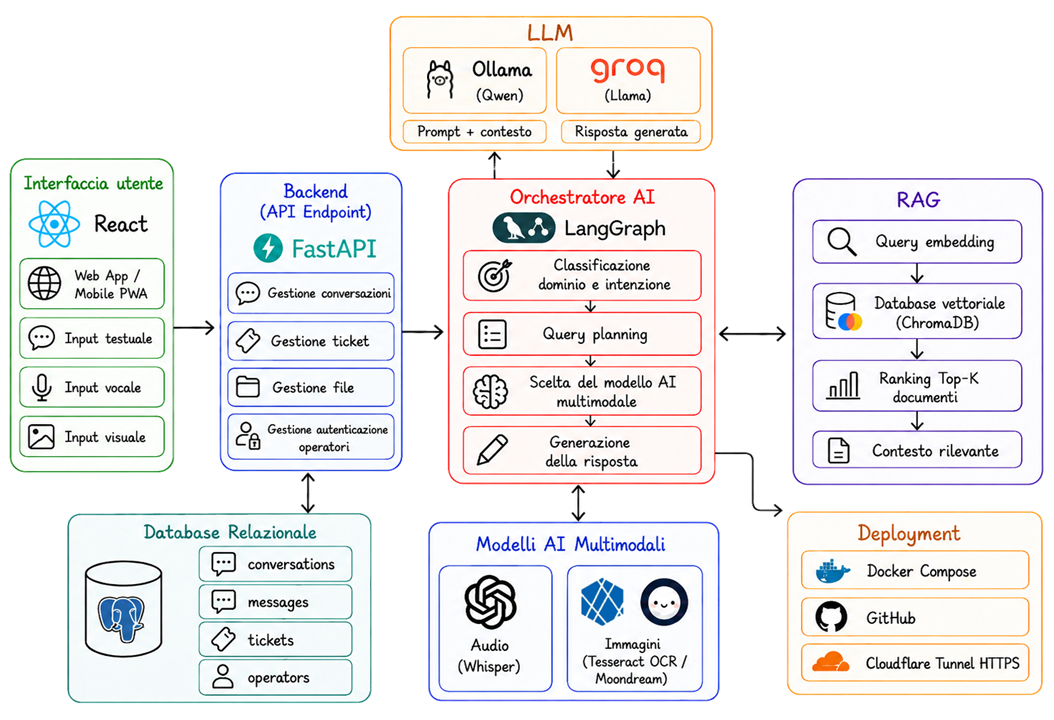
\includegraphics[width=\textwidth]{images/architecture.png}
\caption{Architettura generale del sistema.}
\label{fig:system-architecture}
\end{figure}

I principali componenti dell’architettura sono i seguenti:

\begin{itemize}

\item \textbf{Frontend:} rappresenta il punto di accesso dell’utente al sistema. Gestisce la chat multilingua, l’invio di messaggi testuali, il caricamento delle immagini, l’input vocale e le principali interazioni con l’interfaccia. Include inoltre la dashboard operatore per la gestione dei ticket e la pagina dedicata all’aggiornamento della knowledge base.

\item \textbf{Backend:} costituisce il livello di coordinamento dell’applicazione. Espone gli endpoint API necessari per ricevere le richieste dal frontend, gestisce la logica applicativa, coordina i servizi AI e comunica con i database. Inoltre, demanda a LangGraph l’orchestrazione della pipeline multimodale.

\item \textbf{Database relazionale:} PostgreSQL conserva i dati operativi del sistema, come conversazioni, messaggi, ticket e dati degli operatori. Questo livello garantisce la persistenza delle interazioni e consente di analizzare successivamente le informazioni raccolte.

\item \textbf{Knowledge base e database vettoriale:} la knowledge base contiene le informazioni strutturate relative al dominio dei Giochi del Mediterraneo. Tali contenuti vengono indicizzati in ChromaDB, che conserva la rappresentazione vettoriale dei documenti e consente il recupero semantico delle informazioni più pertinenti rispetto alla richiesta dell’utente.

\item \textbf{Pipeline RAG:} la pipeline di Retrieval-Augmented Generation recupera i documenti rilevanti dalla knowledge base e li fornisce come contesto al modello linguistico. In questo modo la risposta generata è fortemente vincolata dalle fonti individuate.

\item \textbf{Modelli AI:} i modelli AI gestiscono la generazione linguistica, la trascrizione audio, l’estrazione di testo dalle immagini e la descrizione visuale. In particolare, il sistema può utilizzare un LLM locale tramite Ollama oppure un provider API esterno, affiancando moduli come Whisper, Tesseract OCR e Moondream per la gestione della multimodalità.

\item \textbf{Deployment:} Docker Compose collega i diversi servizi e rende l’ambiente riproducibile e containerizzato. Cloudflare Tunnel consente invece di rendere accessibile la demo tramite HTTPS, facilitando il test da dispositivi mobili senza predisporre un’infrastruttura cloud proprietaria.

\end{itemize}

\subsection*{Flusso applicativo}

Il funzionamento del sistema può essere descritto attraverso il flusso end-to-end rappresentato in Figura~\ref{fig:flusso-applicativo}.

\begin{figure}[H]
\centering
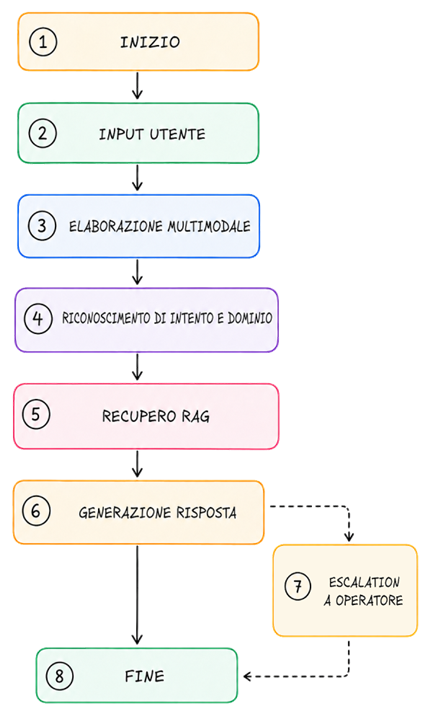
\includegraphics[width=0.4\textwidth]{images/flux.png}
\caption{Flusso applicativo del sistema.}
\label{fig:flusso-applicativo}
\end{figure}

Le fasi che si susseguono durante l'esecuzione sono le seguenti:

\begin{enumerate}
\item \textbf{Avvio della conversazione:} l’utente avvia una conversazione attraverso la chat. Il frontend raccoglie l’input e lo invia al backend insieme alle informazioni di sessione e alla lingua dell’interfaccia.

\item \textbf{Gestione della sessione:} il backend verifica l’esistenza della conversazione e, se necessario, ne crea una nuova. Il messaggio dell’utente viene salvato nel database, così da garantire la tracciabilità dell’interazione fin dall’inizio del processo.

\item \textbf{Elaborazione dell’input:} il contenuto viene gestito da LangGraph in base al formato ricevuto. Se l’utente invia un messaggio testuale, il testo viene inoltrato direttamente alla pipeline. Se invia un audio, il file viene salvato temporaneamente e trascritto tramite il servizio di \textit{speech-to-text}. Se invia un’immagine, il file viene salvato, analizzato tramite OCR e, quando necessario, descritto da un modello visuale. Anche il caricamento dei file multimediali viene tracciato nel database relazionale.

\item \textbf{Riconoscimento di intento e dominio:} il backend analizza la richiesta per individuare lingua, intento, dominio informativo ed entità rilevanti, come discipline sportive, sedi, date o riferimenti geografici. Questa fase consente di capire quale tipo di informazione l’utente stia cercando e se la richiesta può essere gestita attraverso la knowledge base.

\item \textbf{Retrieval semantico:} se la richiesta appartiene a un dominio noto, il sistema interroga ChromaDB per recuperare i documenti più pertinenti. I contenuti recuperati vengono selezionati e utilizzati per costruire il contesto informativo da fornire al modello linguistico.

\item \textbf{Generazione della risposta:} il modello linguistico riceve la richiesta dell’utente insieme al contesto recuperato dalla knowledge base. Sulla base di queste informazioni produce una risposta in linguaggio naturale, coerente con le fonti disponibili e, quando necessario, nella lingua dell’utente.

\item \textbf{Post-processing e controllo:} prima della restituzione all’utente, la risposta viene sottoposta a una fase di controllo. In questa fase vengono gestite le fonti, eventuali collegamenti utili e riferimenti geografici. Se il sistema rileva che la risposta non può essere fornita con sufficiente sicurezza, può suggerire il passaggio all’operatore.

\item \textbf{Restituzione della risposta:} nel ramo principale, la risposta viene mostrata all’utente nella chat. Contestualmente, il messaggio del bot viene salvato nel database insieme alle fonti utilizzate e all’eventuale feedback booleano espresso dall’utente.

\item \textbf{Escalation verso operatore:} nel ramo secondario, l’escalation può attivarsi in due casi principali: quando l’utente richiede esplicitamente supporto umano oppure quando il sistema riconosce di non poter rispondere in modo sufficientemente affidabile. L’escalation può inoltre essere avviata in seguito a un feedback negativo dell’utente rispetto a una risposta già generata.

\item \textbf{Creazione del ticket:} prima di salvare il ticket, il sistema analizza la conversazione, il dominio e la priorità della richiesta. Il ticket generato contiene le informazioni essenziali per la presa in carico da parte dell’operatore, tra cui il riassunto della conversazione generato tramite LLM.

\end{enumerate}

\section{Database relazionale}

Nel sistema T.A.L.O.S. il database relazionale ha il compito di conservare tutti i dati operativi generati durante l’utilizzo dell’applicazione. Nell'ambito della containerizzazione, i dati vengono mantenuti persistenti attraverso un volume Docker dedicato, in modo da non perdere i dati al riavvio dei container. Lo schema iniziale viene inoltre creato automaticamente tramite il file \textit{backend/db/init.sql}, montato nella directory di inizializzazione del servizio PostgreSQL.

L’accesso al database è gestito dal backend FastAPI. All’avvio dell’applicazione, la funzione di inizializzazione verifica la disponibilità della connessione e prepara l’ambiente di persistenza. La logica di accesso ai dati è organizzata in un modulo repository, così da evitare la distribuzione diretta delle query SQL all’interno degli endpoint API. Questa scelta rende il codice più ordinato e separa la logica di comunicazione con il database dalla logica applicativa del backend.

Lo schema logico del database è riportato in Figura~\ref{fig:er-diagram}.

\begin{figure}[H]
\centering
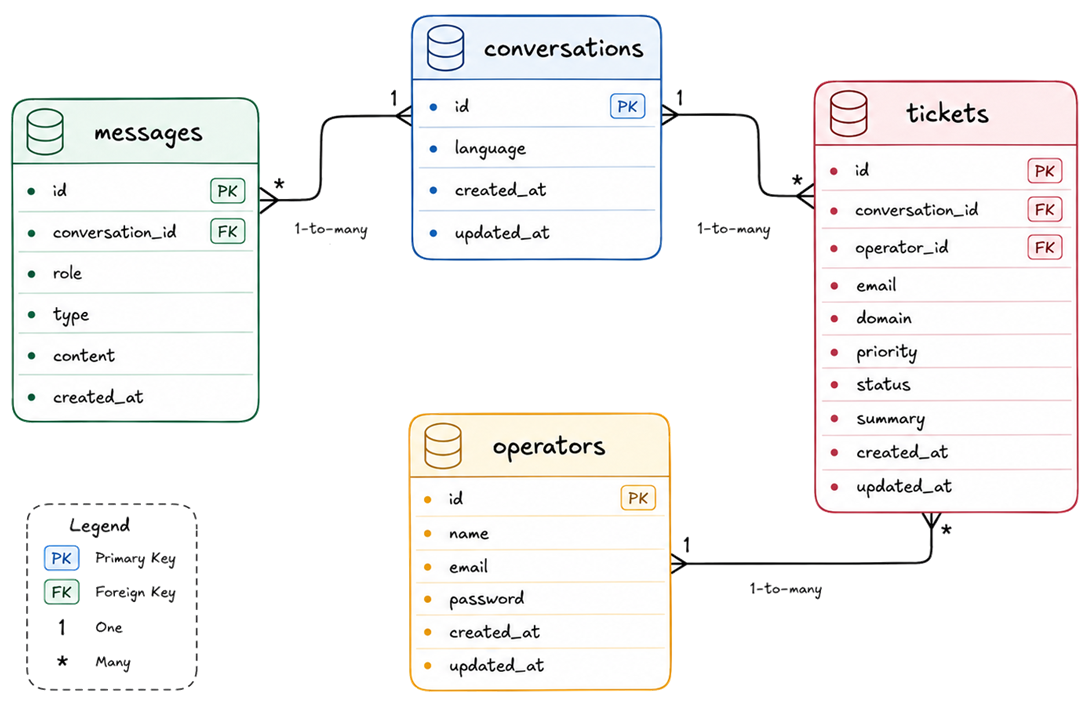
\includegraphics[width=\textwidth]{images/er_diagram.png}
\caption{Diagramma entità-relazioni del database relazionale.}
\label{fig:er-diagram}
\end{figure}

\subsection*{Operatori}

La tabella \textit{operators} è utilizzata per gestire gli operatori autorizzati ad accedere alla dashboard riservata. Nel contesto del sistema, questa tabella consente di distinguere l’utente finale, che interagisce con il chatbot, dall’operatore di customer care, che prende in carico i ticket generati dal sistema.

Ogni operatore è identificato da un identificativo, da un indirizzo e-mail univoco e da una password memorizzata in forma hashata. Questa struttura permette di proteggere l’accesso alle funzionalità riservate e costituisce la base per una futura estensione con ruoli, permessi differenziati e gestione amministrativa degli account.

\subsection*{Conversazioni}

La tabella \textit{conversations} rappresenta le sessioni del chatbot. Ogni conversazione corrisponde a un’interazione avviata dall’utente e costituisce il contenitore logico all’interno del quale vengono raccolti messaggi, feedback ed eventuali escalation.

Questa tabella è importante perché consente al sistema di mantenere il contesto della conversazione nel tempo. Quando l’utente riapre l’applicazione o continua una sessione esistente, il backend può recuperare la conversazione associata allo stesso identificativo di sessione e ricostruire il flusso precedente. In questo modo, l’interazione non viene trattata come una sequenza di messaggi isolati, ma come un dialogo persistente.

\subsection*{Messaggi}

La tabella \textit{messages} conserva i messaggi scambiati durante la conversazione. Ogni record è associato a una conversazione tramite \textit{conversation\_id} e contiene informazioni come ruolo, tipo, contenuto testuale, fonti e feedback.

Il campo \textit{role} distingue i messaggi dell’utente da quelli del bot, mentre il campo \textit{type} permette di distinguere testo, immagine e audio. Questa distinzione è necessaria perché il sistema supporta input multimodali e deve poter tracciare la natura del contenuto ricevuto. Inoltre, la memorizzazione delle fonti associate ai messaggi del bot consente di mantenere la tracciabilità delle risposte generate tramite RAG.

La relazione tra \textit{conversations} e \textit{messages} è di tipo uno-a-molti: una conversazione può contenere molti messaggi, mentre ogni messaggio appartiene a una sola conversazione. Le chiavi esterne verso \textit{conversations} sono configurate con cancellazione a cascata, in modo da mantenere la coerenza dello schema anche nel caso in cui una conversazione venga rimossa.

\subsection*{Ticket}

La tabella \textit{tickets} gestisce il passaggio dal supporto automatico al supporto umano.

Ogni ticket è associato a una conversazione tramite \textit{conversation\_id} e contiene informazioni come stato, priorità, dominio, e-mail dell’utente e riassunto della richiesta. Il campo \textit{escalated\_message\_id} permette di collegare il ticket al messaggio del bot da cui ha avuto origine l’escalation. In questo modo, l’operatore non riceve una richiesta isolata, ma può ricostruire il contesto che ha portato all’apertura del ticket.

Anche la relazione tra \textit{conversations} e \textit{tickets} è di tipo uno-a-molti. Una singola conversazione può infatti generare più ticket in momenti diversi, ad esempio se l’utente formula richieste distinte oppure se nel corso della stessa sessione emergono più criticità non risolvibili automaticamente.

\subsection*{pgAdmin}

Il database è integrato anche con pgAdmin, un servizio dedicato alla gestione visuale di PostgreSQL, come mostrato in Figura~\ref{fig:pgadmin}. Esso consente di ispezionare le tabelle, visualizzare i record salvati ed eseguire query SQL tramite interfaccia grafica.

Questa interfaccia si è rivelata utile durante lo sviluppo e il testing perché ha facilitato la verifica delle informazioni memorizzate..

\begin{figure}[H]
\centering
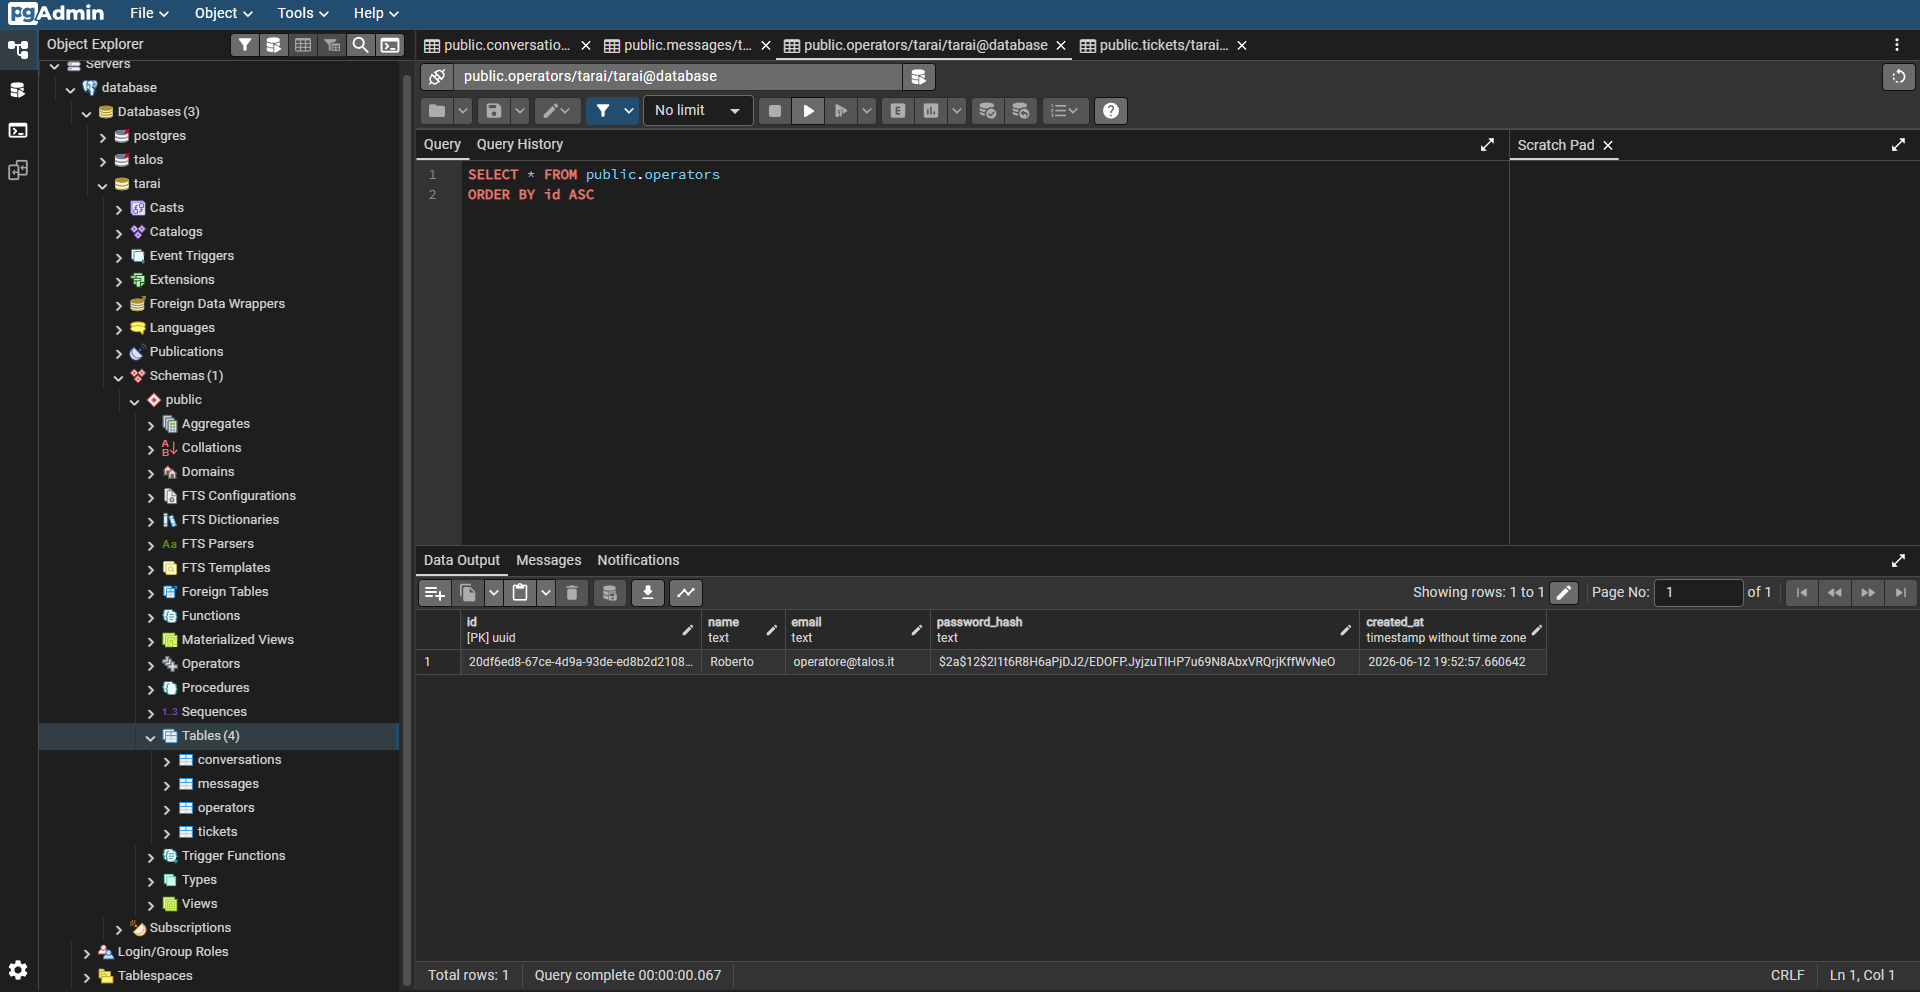
\includegraphics[width=\textwidth]{images/pgadmin.png}
\caption{Interfaccia pgAdmin utilizzata per l’ispezione delle tabelle nel database PostgreSQL.}
\label{fig:pgadmin}
\end{figure}

\section{Backend}

Il backend rappresenta il livello applicativo centrale del sistema. Ha il compito di ricevere le richieste provenienti dal frontend, validare i dati in ingresso, coordinare i servizi interni, comunicare con il database relazionale e invocare i moduli di AI necessari alla generazione della risposta.

FastAPI consente di generare automaticamente la documentazione OpenAPI degli endpoint del backend. Come mostrato in Figura~\ref{fig:backend-openapi}, le route possono essere consultate attraverso l’interfaccia Swagger, che le organizza per gruppi funzionali. Questo strumento è utile durante lo sviluppo perché permette di testare rapidamente le API senza passare dal frontend e di verificare che i contratti tra frontend e backend siano stati implementati correttamente.

\begin{figure}[H]
\centering
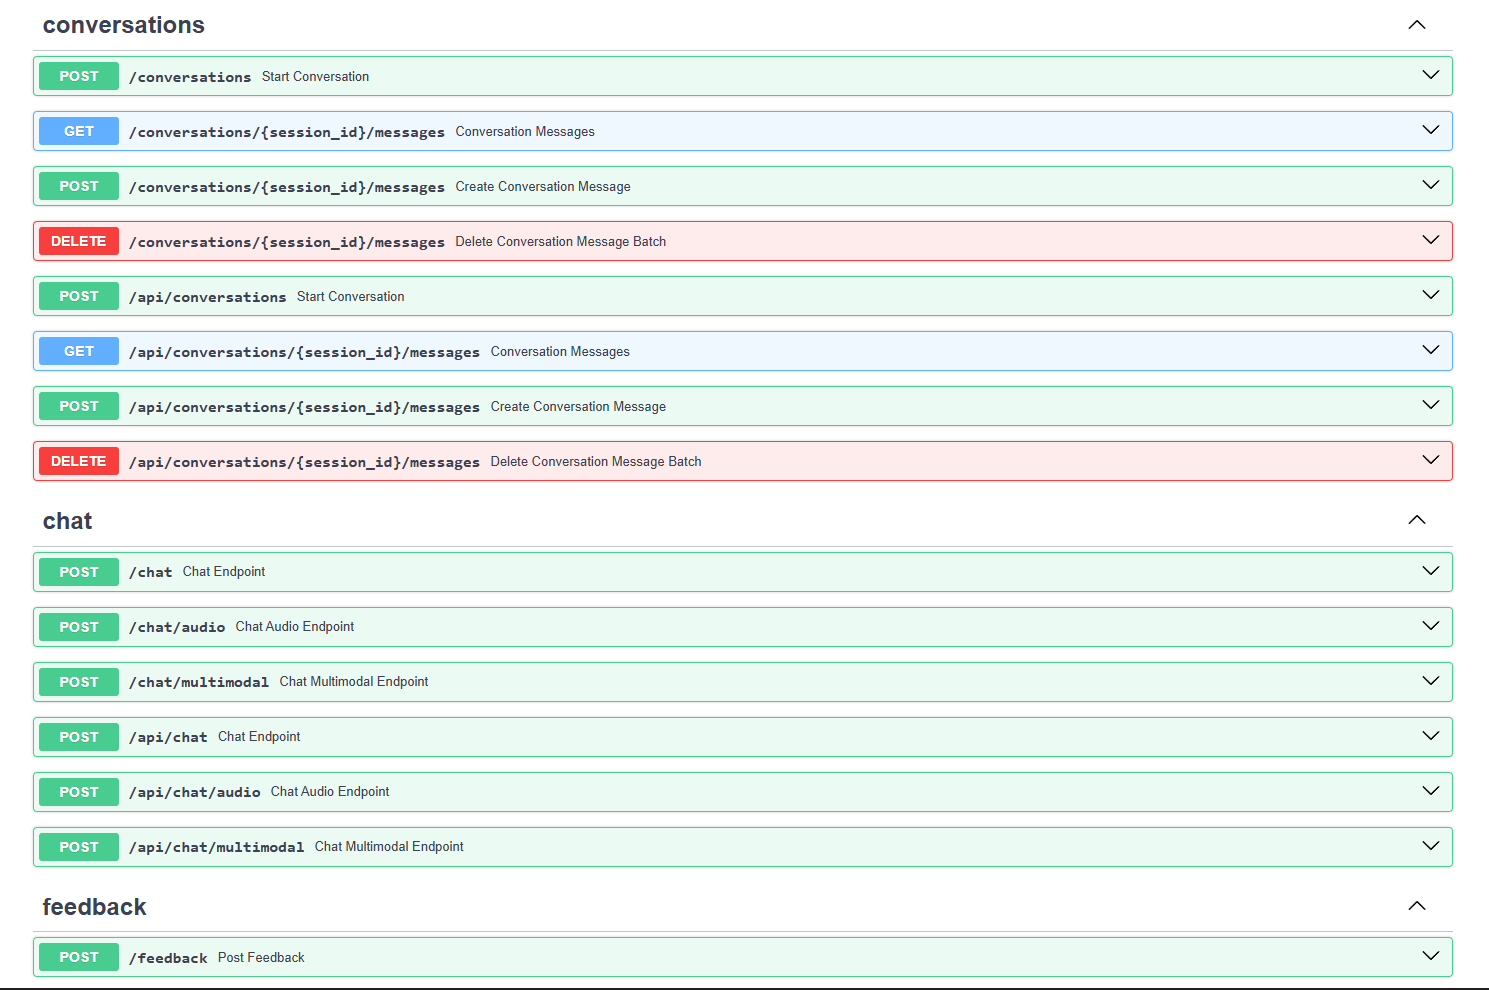
\includegraphics[width=\textwidth]{images/opendocs.png}
\caption{Documentazione Swagger/OpenAPI generata automaticamente dal backend FastAPI.}
\label{fig:backend-openapi}
\end{figure}

\subsection*{Route di health check}

L’endpoint \textit{/api/health} permette di verificare lo stato generale del backend. Questa route restituisce informazioni utili sul funzionamento della pipeline RAG, come lo stato della knowledge base, il numero di documenti presenti nella collection, il modello di embedding configurato e il modello LLM utilizzato.

Questo endpoint è utile soprattutto durante lo sviluppo e il testing, perché consente di controllare rapidamente se il backend è attivo e se la knowledge base è stata inizializzata correttamente. Inoltre, viene usato anche nell’ambiente containerizzato per verificare che il servizio backend sia pronto a ricevere richieste.

\subsection*{Route per la chat testuale}

La route principale per l’interazione testuale è \textit{/api/chat}. Essa viene utilizzata quando l’utente invia un messaggio scritto dalla chat. In questo caso, il backend riceve il testo, le informazioni di sessione e la lingua dell’interfaccia, quindi verifica l’esistenza della conversazione o ne crea una nuova se necessario.

Il messaggio dell’utente viene salvato nel database relazionale prima dell’elaborazione della risposta, così da garantire la tracciabilità dell’interazione. Successivamente, la richiesta viene inoltrata al flusso orchestrato tramite LangGraph, che si occupa di pianificazione della query, recupero dei documenti rilevanti dalla knowledge base, generazione della risposta e post-processing finale.

La route \textit{/api/chat} rappresenta quindi il punto di ingresso standard del chatbot e gestisce il caso più diretto: una domanda testuale che viene trasformata in una risposta testuale basata sulle informazioni recuperate tramite RAG.

\subsection*{Route per i messaggi vocali}

I messaggi vocali vengono gestiti tramite la route \textit{/api/chat/audio}. Questa route consente all’utente di inviare un file audio invece di un messaggio scritto. Il backend riceve il file, verifica che il contenuto sia effettivamente di tipo audio, lo salva temporaneamente nella cartella degli upload e lo invia al servizio di trascrizione.

La trascrizione viene effettuata tramite un modulo di \textit{speech-to-text}, così da trasformare il contenuto vocale in testo. Se la trascrizione non produce un risultato utilizzabile, il sistema gestisce il caso come audio incomprensibile. Una volta ottenuta la trascrizione, il sistema riconduce l’audio alla stessa logica della chat testuale.

Il file audio salvato viene collegato alla conversazione tramite un riferimento statico nella forma \textit{/api/uploads/{filename}}. In questo modo, il contenuto multimediale resta associato all’interazione e può essere recuperato dal frontend quando necessario.

\subsection*{Route per input multimodali}

Le richieste contenenti immagini o file multimodali vengono gestite tramite la route \textit{/api/chat/multimodal}. Questa route è utilizzata quando l’utente invia un contenuto non puramente testuale, ad esempio un’immagine, uno screenshot o un file da analizzare. La stessa route può gestire anche audio, ma nel sistema viene mantenuta anche la route specifica \textit{/api/chat/audio} per il caso vocale.

Nel caso di immagini, il backend salva il file ricevuto e lo sottopone a elaborazione tramite OCR e, quando necessario, tramite un modello visuale. L’OCR consente di estrarre eventuale testo presente nell’immagine, mentre il modello visuale permette di produrre una descrizione del contenuto quando l’informazione non è soltanto testuale. Il sistema costruisce quindi un contesto visuale interno, composto dalla descrizione dell’immagine e dal testo eventualmente estratto.

La route multimodale ha quindi il compito di normalizzare input eterogenei e trasformarli in una forma compatibile con la pipeline RAG. In questo modo, testo, audio e immagini non generano tre sistemi separati, ma confluiscono in un unico processo applicativo controllato.

\subsection*{Route per la gestione delle conversazioni}

Il backend espone anche route dedicate alla gestione delle conversazioni. L’endpoint \textit{/api/conversations}, con metodo POST, consente di creare o recuperare una conversazione a partire da un identificativo di sessione. Se il frontend non fornisce un identificativo, il backend può generarne uno nuovo, associandolo a una nuova sessione del chatbot.

L’endpoint \textit{/api/conversations/session\_id/messages}, con metodo GET, consente di recuperare i messaggi già salvati all’interno di una conversazione. Questa funzionalità permette al frontend di ricostruire lo storico della chat, ad esempio quando l’utente ricarica la pagina o riapre l’applicazione con lo stesso identificativo di sessione.

Lo stesso endpoint, con metodo POST, permette di salvare un messaggio associato a una conversazione. Il messaggio può avere ruolo \textit{user} oppure \textit{bot} e può essere di tipo testuale, immagine o audio. Con metodo DELETE, invece, l’endpoint permette di eliminare un insieme di messaggi identificati tramite i rispettivi identificativi.

\subsection*{Route per feedback e tracciamento delle risposte}

Il backend espone route dedicate alla gestione del feedback dell’utente. L’endpoint \textit{/api/feedback}, con metodo POST, registra un feedback associato a una risposta del bot.

L’endpoint \textit{/api/messages/message\_id/feedback}, con metodo PATCH, aggiorna invece il valore di soddisfazione associato a uno specifico messaggio. Nel progetto, il feedback viene collegato ai messaggi del bot, perché l’utente valuta la risposta ricevuta e non il proprio messaggio.

\subsection*{Route per ticket ed escalation}

Le route relative ai ticket gestiscono il passaggio dal supporto automatico al supporto umano. L’endpoint pubblico principale è \textit{/api/tickets}, con metodo POST. Esso viene utilizzato quando una conversazione deve essere trasformata in una richiesta gestibile da un operatore.

Prima della creazione del ticket, il backend valida l’indirizzo e-mail dell’utente e verifica l’esistenza della conversazione associata. Successivamente, il sistema esegue una fase di \textit{triage} tramite i servizi interni, analizzando la conversazione e il messaggio che ha generato l’escalation. Da questa analisi vengono ricavati dominio, priorità e riassunto della richiesta.

\subsection*{Route per la dashboard operatore}

La dashboard operatore utilizza endpoint protetti da autenticazione tramite token \textit{Bearer}. L’endpoint \textit{/api/operator/login} consente all’operatore di autenticarsi tramite e-mail e password. Se le credenziali sono corrette, il backend restituisce un token di accesso e i dati essenziali dell’operatore. L’endpoint \textit{/api/operator/logout} gestisce invece la chiusura della sessione lato client, mentre \textit{/api/operator/me} restituisce il profilo dell’operatore autenticato.

Per la gestione dei ticket, la dashboard utilizza \textit{/api/operator/tickets}, che restituisce la lista dei ticket disponibili. La route supporta filtri opzionali per stato, priorità e dominio, così da permettere all’operatore di concentrarsi sulle richieste più rilevanti. L’endpoint \textit{/api/operator/tickets/ticket\_id} consente invece di recuperare il dettaglio di un singolo ticket, includendo le informazioni della conversazione associata.

Sono presenti anche endpoint di supporto operativo basati su LLM. La route \textit{/api/operator/tickets/ticket\_id/translate} permette di tradurre la conversazione del ticket, funzionalità utile quando l’utente ha interagito in una lingua diversa dall’italiano. La route \textit{/api/operator/tickets/ticket\_id/email-draft} genera una bozza di risposta e-mail, offrendo all’operatore un testo iniziale da rivedere e inviare. Infine, \textit{/api/operator/tickets/ticket\_id/status}, con metodo PATCH, consente di aggiornare lo stato del ticket.

\subsection*{Route per la gestione della knowledge base}

Il backend espone anche route riservate alla gestione della knowledge base. L’endpoint \textit{/api/knowledge/options} restituisce i domini e le tipologie di record ammesse dal sistema. Questa route è utile per popolare correttamente i campi del form di inserimento, evitando valori non coerenti con la struttura prevista.

L’endpoint \textit{/api/knowledge/records}, con metodo POST, consente invece di aggiungere un nuovo record informativo alla knowledge base. Il payload contiene campi come titolo, dominio, tipologia, fonte, documento, eventuale indirizzo, coordinate geografiche e metadati. Dopo l’inserimento, il record viene anche indicizzato nella collection vettoriale, così da renderlo immediatamente disponibile per il retrieval.

Queste route consentono di aggiornare la base informativa senza modificare manualmente i file del progetto. In questo modo, la knowledge base diventa più facilmente mantenibile e può essere estesa anche durante l’evoluzione del sistema.

\section{AI e multimodalità}

Poiché il sistema deve gestire testo, audio e immagini, la componente di intelligenza artificiale non è costituita da un singolo modello, ma da più moduli coordinati tra loro.

\subsection*{Configurazione}

Per la configurazione dei modelli AI, è possibile scegliere il provider LLM da utilizzare, poiché il sistema può lavorare in modalità \textit{groq}, \textit{local} oppure \textit{auto}.

In modalità \textit{groq}, le funzionalità AI vengono delegate a servizi API esterni. Questa modalità consente di ottenere tempi di risposta più rapidi e di sfruttare modelli disponibili tramite provider esterno, ma introduce una dipendenza da un servizio remoto e dalla relativa configurazione API.

In modalità \textit{local}, il sistema privilegia invece modelli e strumenti eseguiti localmente. Questa scelta aumenta la replicabilità del progetto e riduce la dipendenza da servizi esterni, ma richiede risorse hardware adeguate e può comportare tempi di risposta più elevati.

In modalità \textit{auto}, il backend prova a utilizzare il provider più adatto o disponibile, mantenendo la possibilità di passare a un’alternativa quando necessario. Questa modalità è utile perché consente al sistema di adattarsi alla disponibilità dei servizi configurati.

In modalità locale è previsto l’uso di Ollama con il modello \textit{qwen3:8b}. Il sistema include anche una logica di \textit{fallback}: se la chiamata al modello locale non risponde entro il tempo previsto o se il servizio non è disponibile, il sistema può passare al provider API, se configurato.

\subsection*{Orchestrazione con LangGraph}

Per coordinare il flusso AI è stato integrato LangGraph, che permette di rappresentare l’elaborazione della richiesta come un grafo di stati. Ogni nodo del grafo ha una responsabilità specifica e restituisce un aggiornamento dello stato condiviso.

Nel progetto, lo stato contiene informazioni come il messaggio dell’utente, la cronologia recente della conversazione, la lingua, l’eventuale contesto visuale, i documenti recuperati, la risposta generata e le fonti da mostrare. Questa struttura consente ai diversi nodi di lavorare su una rappresentazione comune della richiesta, evitando che ogni fase debba ricostruire da zero le informazioni necessarie.

La Figura~\ref{fig:langgraph-nodes} mostra il grafo dei nodi utilizzati nel sistema. Il flusso è lineare e procede da \textit{planner} a \textit{retriever}, poi a \textit{generator} e infine a \textit{postprocess}.

\begin{figure}[H]
\centering
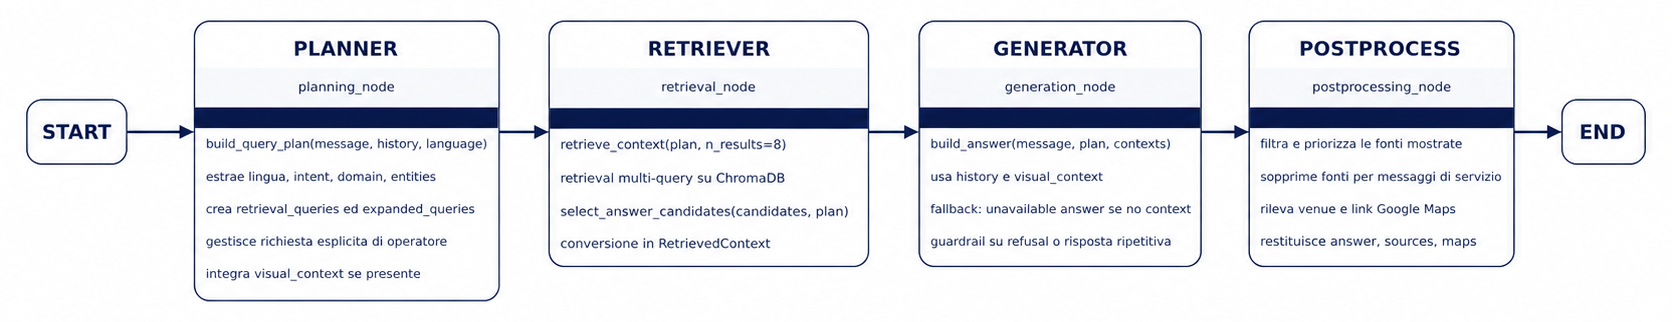
\includegraphics[width=\textwidth]{images/lang.png}
\caption{Sequenza dei nodi LangGraph utilizzata per l’orchestrazione della risposta.}
\label{fig:langgraph-nodes}
\end{figure}

\subsection*{Nodo planner}

Il nodo \textit{planner} rappresenta la prima fase logica del flusso LangGraph. Il suo compito è analizzare il messaggio dell’utente e costruire un piano di ricerca utile per le fasi successive.

In questa fase vengono individuati diversi elementi: la lingua in cui deve essere prodotta la risposta, il dominio informativo della richiesta, l’intento dell’utente, le entità rilevanti e le query da utilizzare per il retrieval. Le entità possono riguardare, ad esempio, discipline sportive, sedi di gara, date, servizi, accessibilità o riferimenti geografici.

Il \textit{planner} ha quindi una funzione di normalizzazione e orientamento. Non genera direttamente la risposta finale, ma prepara il sistema a recuperare i documenti più pertinenti. Inoltre, gestisce alcuni casi particolari, come la richiesta esplicita di parlare con un operatore umano. In presenza di una richiesta di questo tipo, il piano può segnalare la necessità di attivare un flusso di escalation invece di procedere con una normale risposta informativa.

\subsection*{Nodo retriever}

Il nodo \textit{retriever} utilizza il piano prodotto dal \textit{planner} per interrogare la knowledge base tramite ChromaDB. In questa fase, le query individuate vengono confrontate con i documenti indicizzati nel database vettoriale, così da recuperare i contenuti semanticamente più vicini alla richiesta dell’utente.

Il sistema non si limita a restituire un singolo documento, ma recupera più documenti candidati. Successivamente, questi contenuti vengono selezionati in base alla pertinenza e convertiti in contesti utilizzabili dal modello linguistico. Il ruolo del \textit{retriever} è quindi fondamentale perché determina quali informazioni verranno fornite al modello durante la generazione della risposta.

\subsection*{Nodo generator}

Il nodo \textit{generator} produce la risposta finale a partire dal messaggio dell’utente, dal piano costruito dal \textit{planner}, dai documenti recuperati dal \textit{retriever}, dalla cronologia recente e dall’eventuale contesto multimodale. Quando la richiesta è multilingua, il modello produce la risposta nella lingua individuata o richiesta dall’utente.

Il nodo \textit{generator} gestisce anche i casi in cui non siano disponibili documenti sufficientemente pertinenti. In queste situazioni, il sistema può produrre una risposta di indisponibilità del dato, evitando di inventare informazioni.

\subsection*{Nodo postprocess}

Il nodo \textit{postprocess} rappresenta l’ultima fase del flusso prima della restituzione della risposta al frontend. Il suo compito è controllare, rifinire e organizzare l’output generato dal modello linguistico.

In particolare, il nodo filtra e ordina le fonti da mostrare all’utente, così da evitare riferimenti ridondanti o poco pertinenti. Quando la risposta è soltanto un messaggio di servizio, il sistema può sopprimere la visualizzazione delle fonti, perché non è necessario mostrare riferimenti informativi. Inoltre, il nodo individua eventuali venue o luoghi citati nella risposta e, quando disponibili coordinate o indirizzi, genera collegamenti a Google Maps utili per la navigazione.

\section{Frontend}

L'interfaccia frontend è stata progettata in React e stilizzata con TailwindCSS. In generale, il frontend separa le chiamate HTTP dalla logica delle pagine tramite moduli dedicati, come \textit{chatApi.js}, \textit{operatorApi.js} e \textit{knowledgeApi.js}.

La schermata principale della chat, mostrata in Figura~\ref{fig:frontend-chat-light}, presenta l'organizzazione di tutti gli elementi nell'interfaccia, con il riferimento ai Giochi del Mediterraneo, la selezione della lingua, il tema chiaro o scuro, il countdown all’evento e l’area dedicata alla chat. Il layout è stato pensato per mantenere la conversazione al centro dell’esperienza e rendere facilmente raggiungibili le azioni principali.

\begin{figure}[H]
\centering
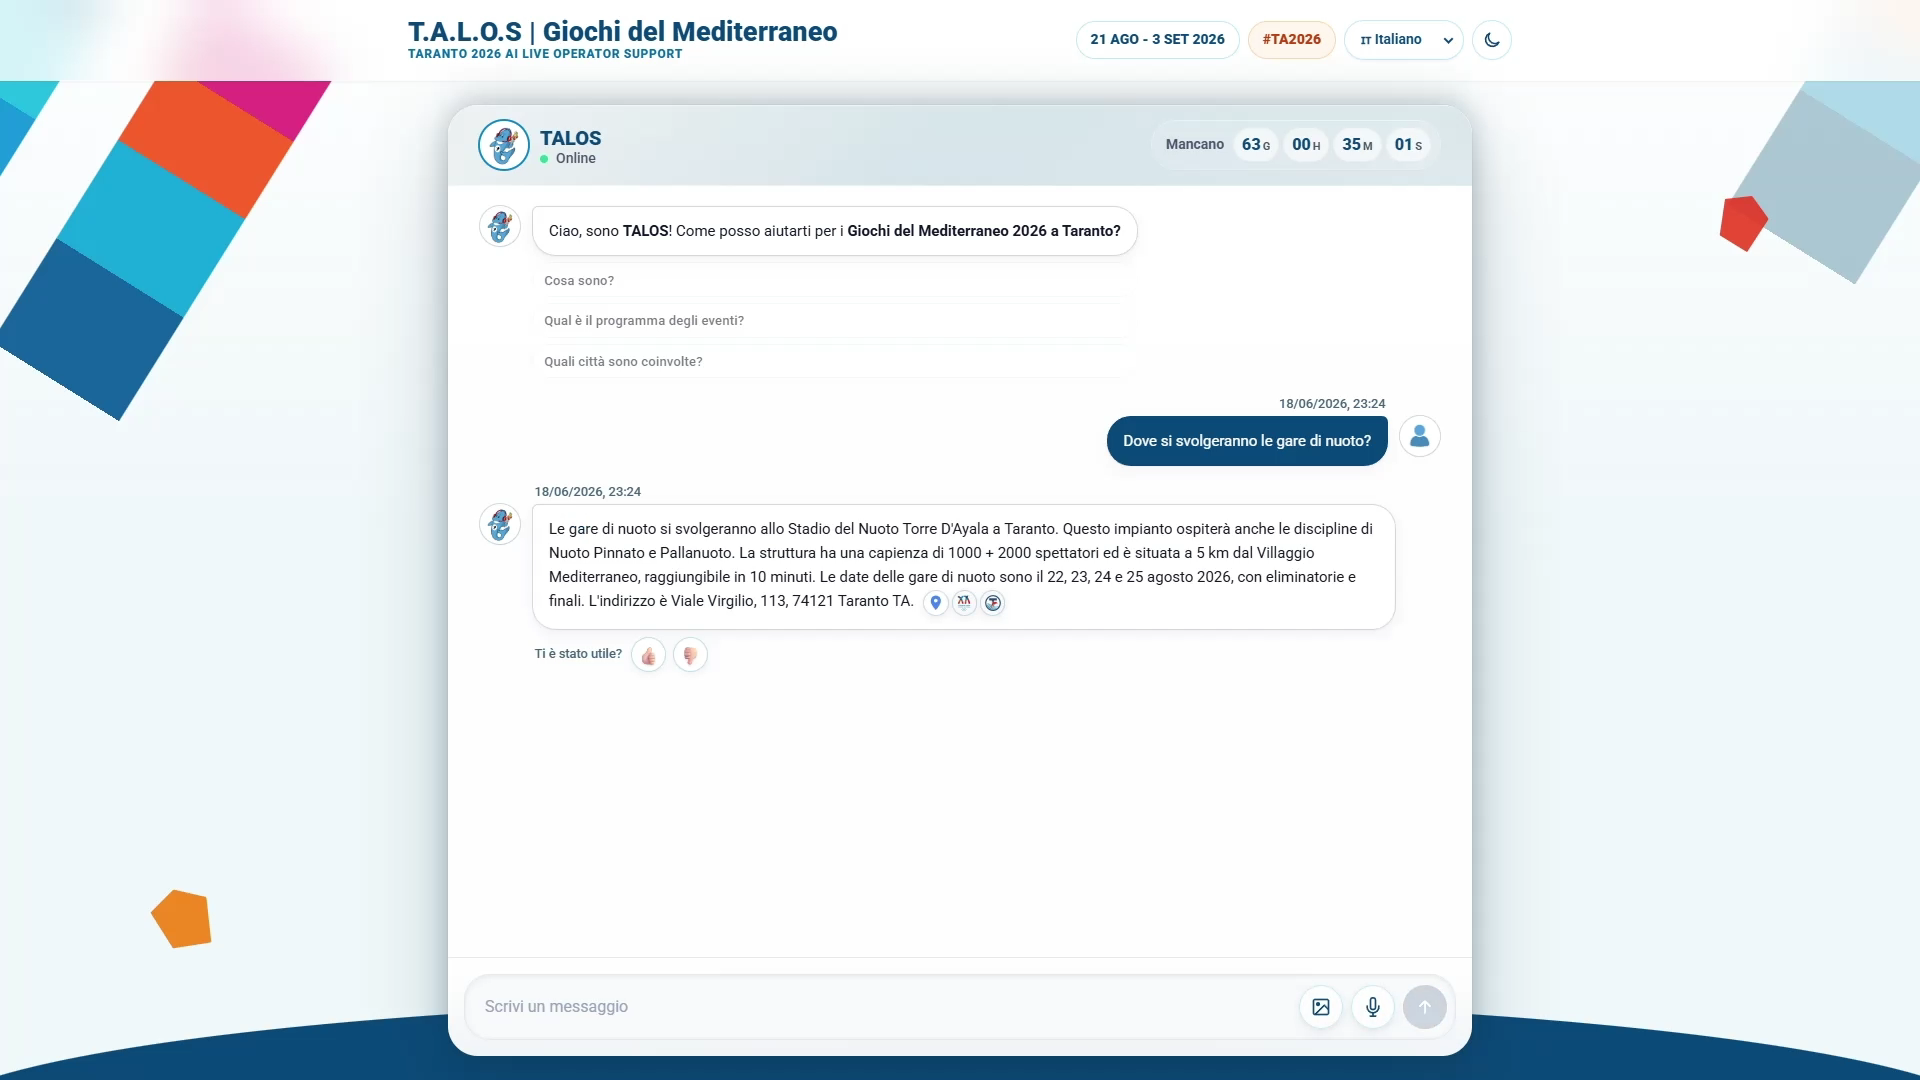
\includegraphics[width=\textwidth]{images/text-light.png}
\caption{Interfaccia principale della chat in tema chiaro.}
\label{fig:frontend-chat-light}
\end{figure}

Il sistema supporta anche il tema scuro, come mostrato in Figura~\ref{fig:frontend-chat-dark}. Questa scelta migliora l’accessibilità dell’interfaccia, soprattutto su dispositivi mobili o in ambienti con scarsa luminosità. La preferenza dell’utente viene mantenuta nel browser, così da rendere l’esperienza consistente anche alla riapertura dell’applicazione. Il sistema già prevede, infatti, il recupero dei messaggi precedenti quando questi sono associati allo stesso identificativo di sessione.

\begin{figure}[H]
\centering
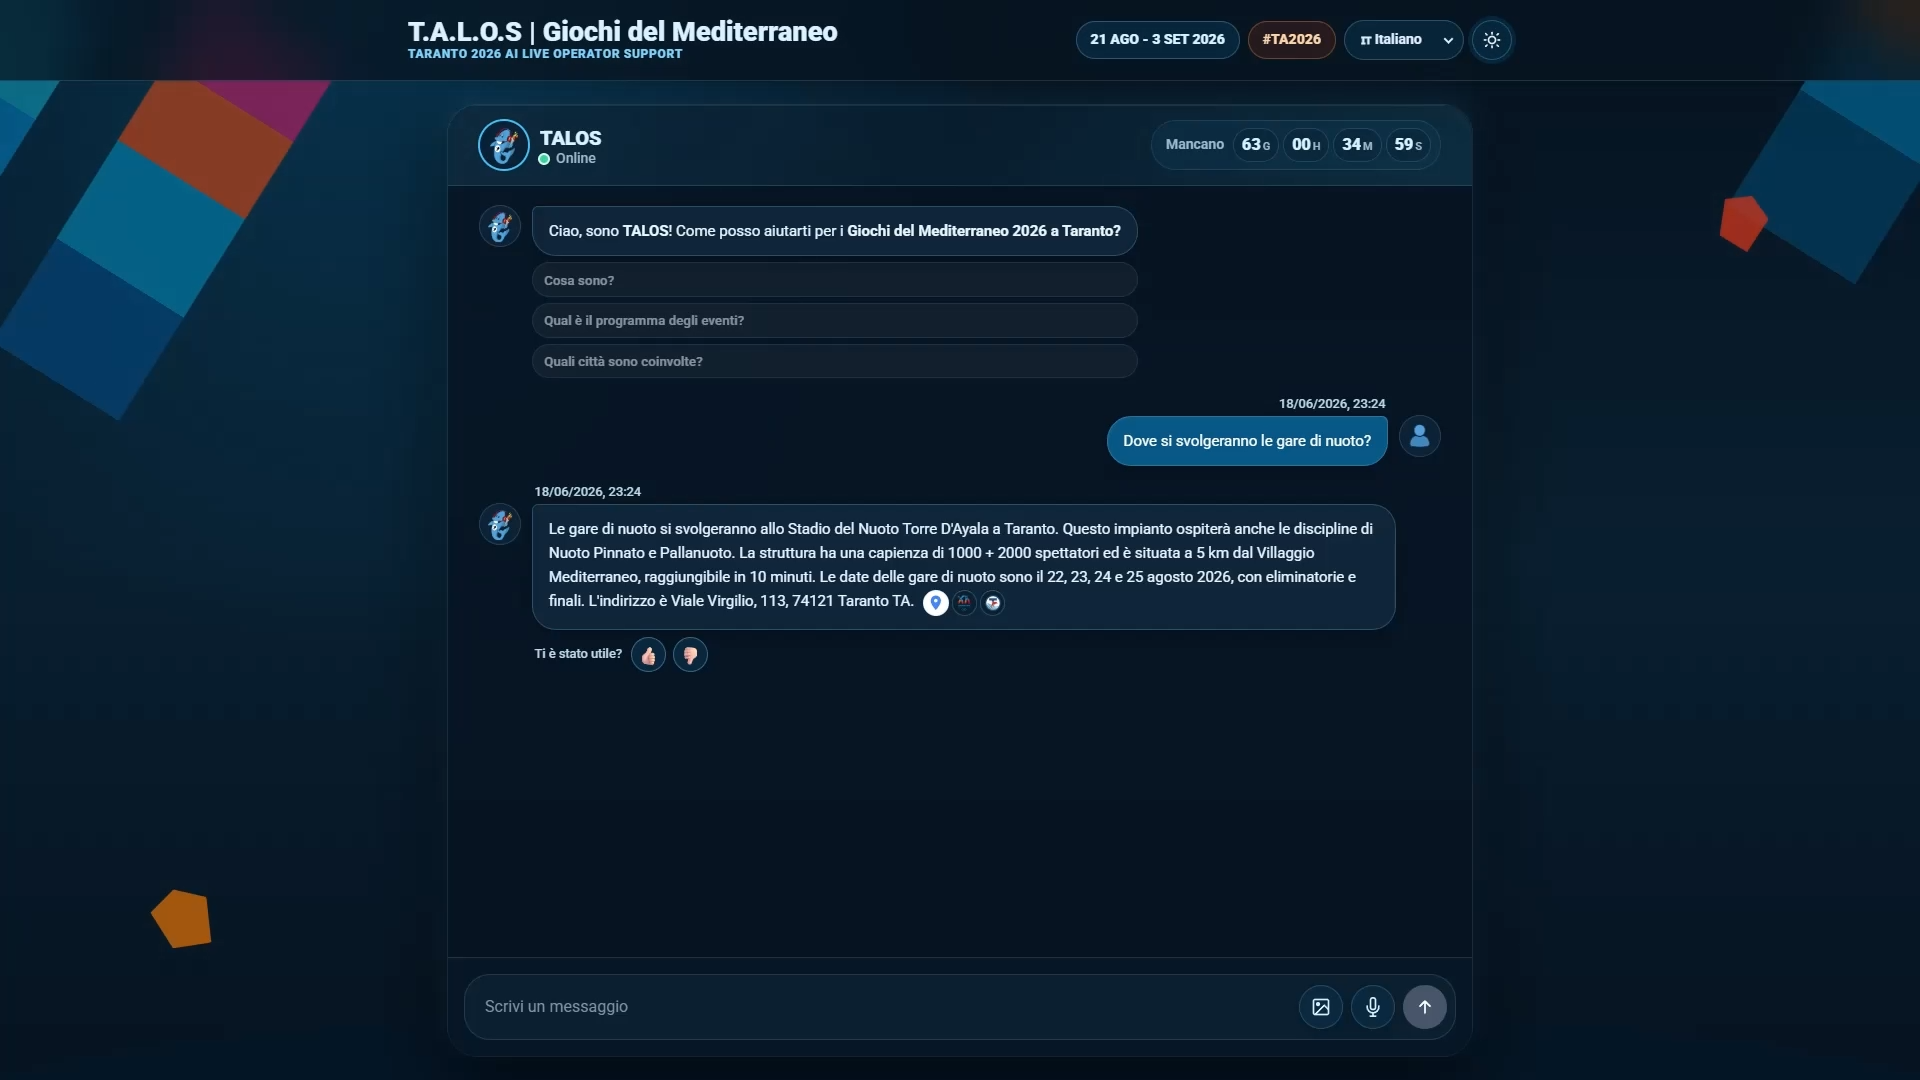
\includegraphics[width=\textwidth]{images/text-dark.png}
\caption{Interfaccia principale della chat in tema scuro.}
\label{fig:frontend-chat-dark}
\end{figure}
Quando si seleziona un'altra lingua o viene riconosciuta una lingua differente dal messaggio dell'utente, il frontend aggiorna in automatico i testi dell’interfaccia in modo coerente. Il backend riceve la lingua selezionata e la utilizza per orientare query planning e generazione della risposta. In questo modo, l’utente può ricevere contenuti nella lingua attesa, evitando discrepanze tra la lingua dell’interfaccia e la lingua della risposta.

La Figura~\ref{fig:frontend-audio-es} mostra un esempio di conversazione in spagnolo con input vocale. Il messaggio audio viene visualizzato nella chat tramite un componente dedicato, con rappresentazione della forma d'onda e durata della registrazione.

\begin{figure}[H]
\centering
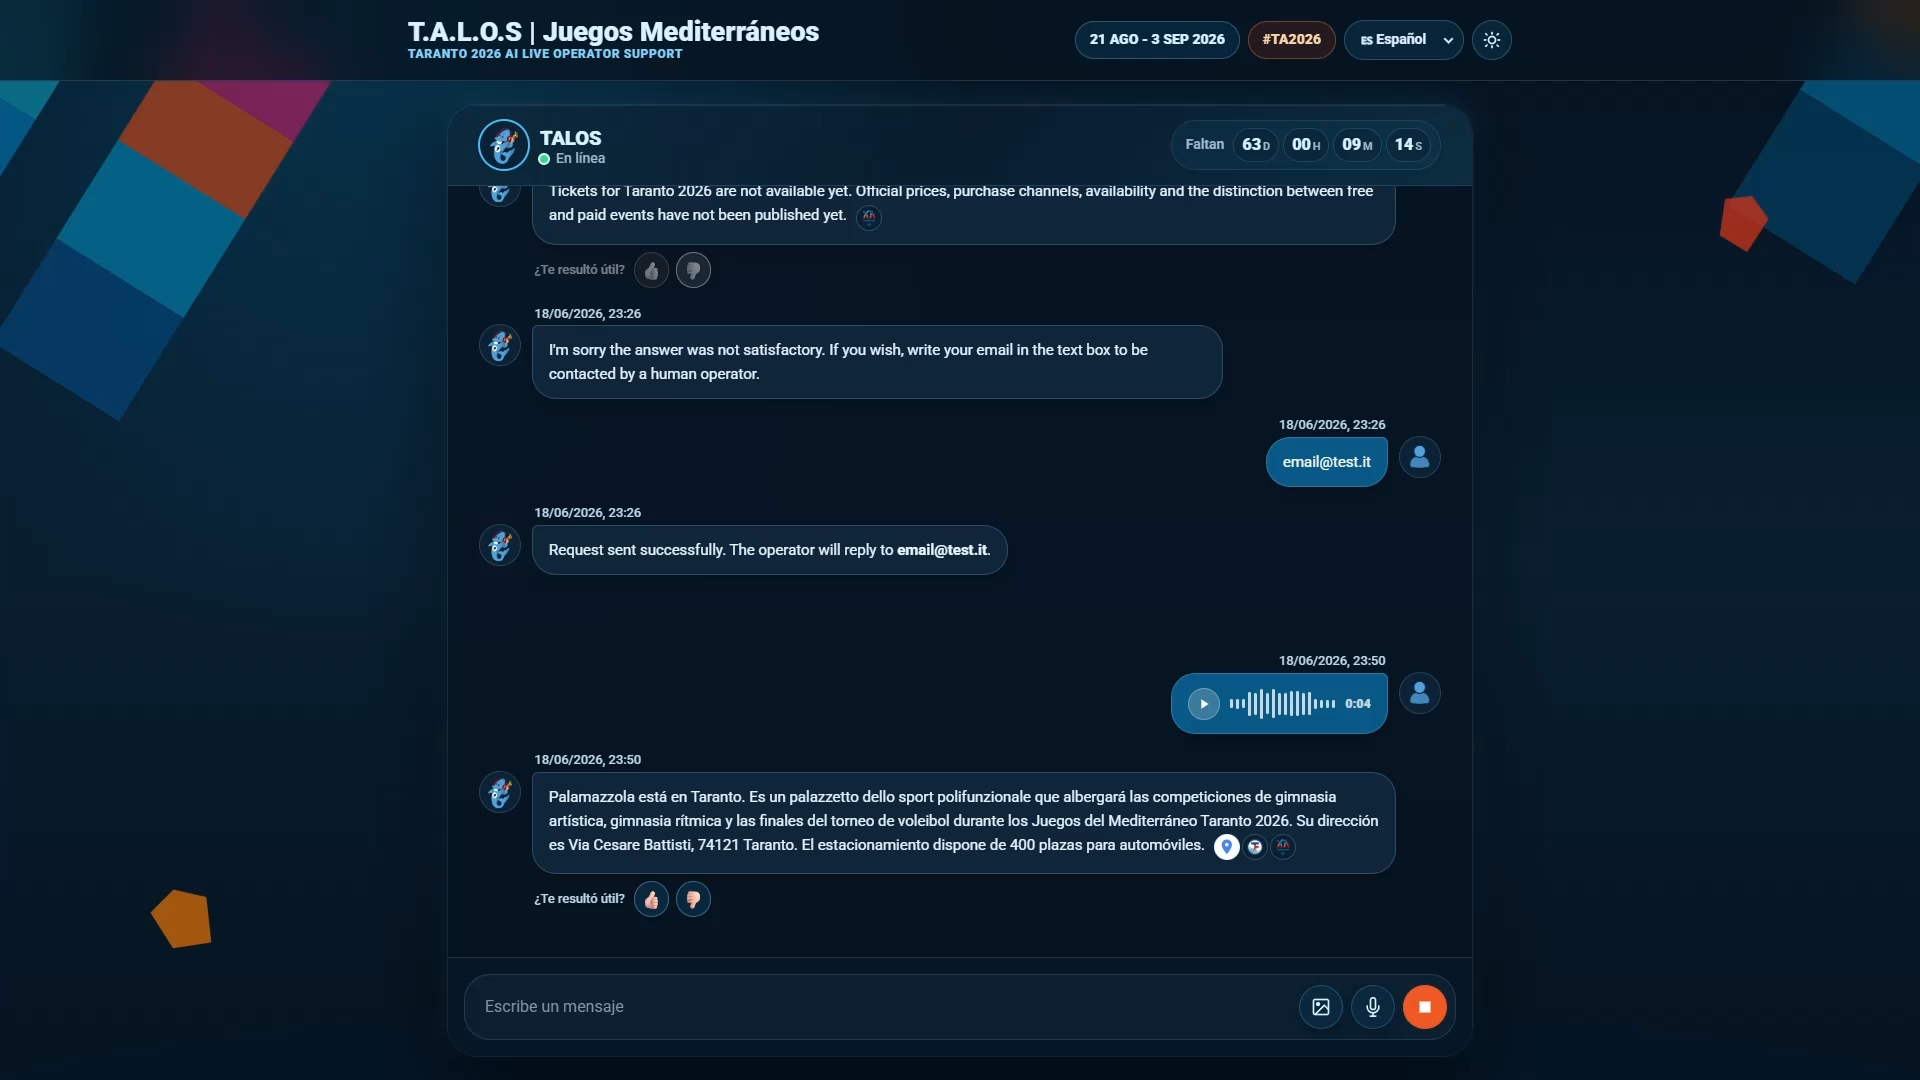
\includegraphics[width=\textwidth]{images/audio-es-dark.png}
\caption{Esempio di interazione vocale in lingua spagnola.}
\label{fig:frontend-audio-es}
\end{figure}

L’interfaccia supporta anche l’invio di immagini. L’utente può caricare un file, trascinarlo nell’area della chat o incollarlo direttamente. Come mostrato in Figura~\ref{fig:frontend-image}, l’immagine viene visualizzata nella chat e deve essere accompagnata obbligatoriamente da un input testuale.

\begin{figure}[H]
\centering
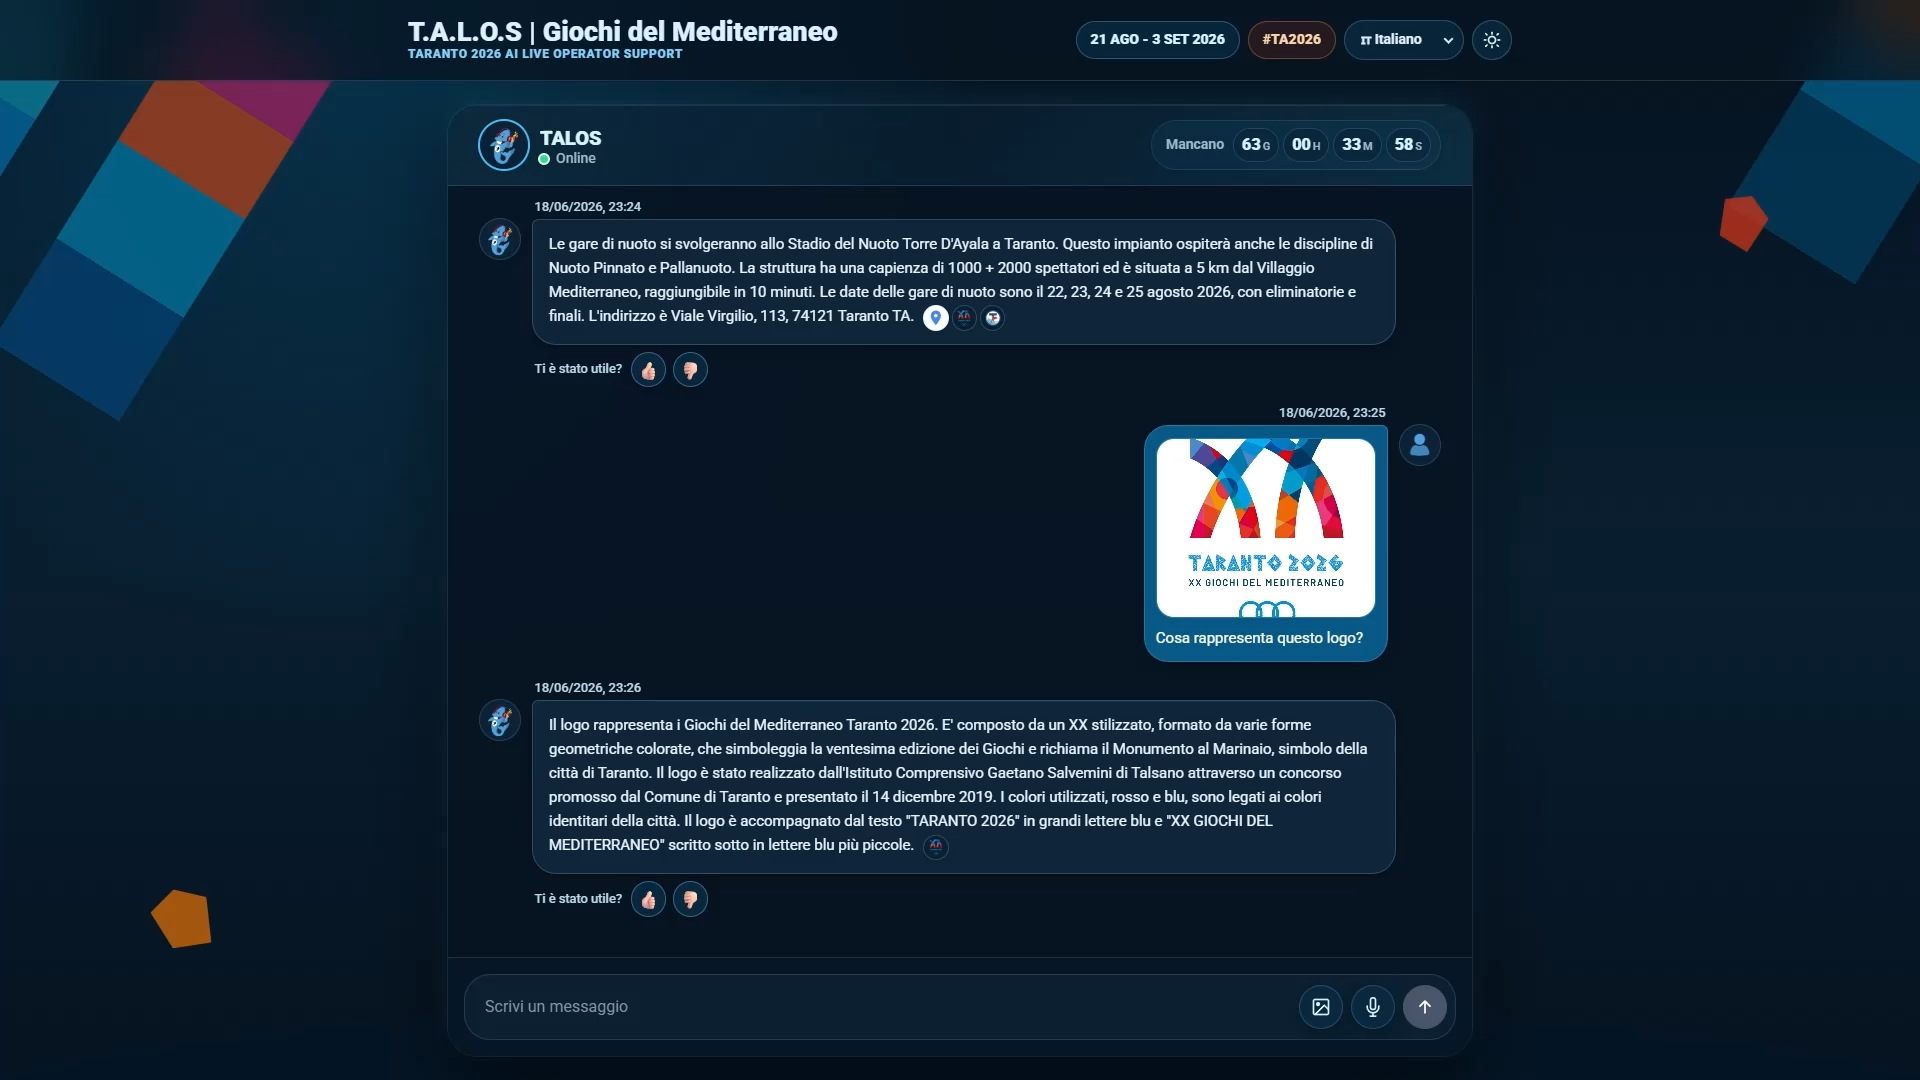
\includegraphics[width=\textwidth]{images/image-dark.png}
\caption{Esempio di richiesta multimodale con immagine allegata.}
\label{fig:frontend-image}
\end{figure}

L’esperienza utente include la possibilità di cliccare sulle fonti, visualizzare data e ora dei messaggi, ingrandire le immagini nella chat, usufruire di suggerimenti iniziali e fornire feedback sui messaggi generati dal bot. In caso di insoddisfazione o richiesta di supporto umano, l’interfaccia guida l’utente verso l’inserimento dell’e-mail e l’apertura di un ticket, come mostrato in Figura~\ref{fig:frontend-escalation}.

\begin{figure}[H]
\centering
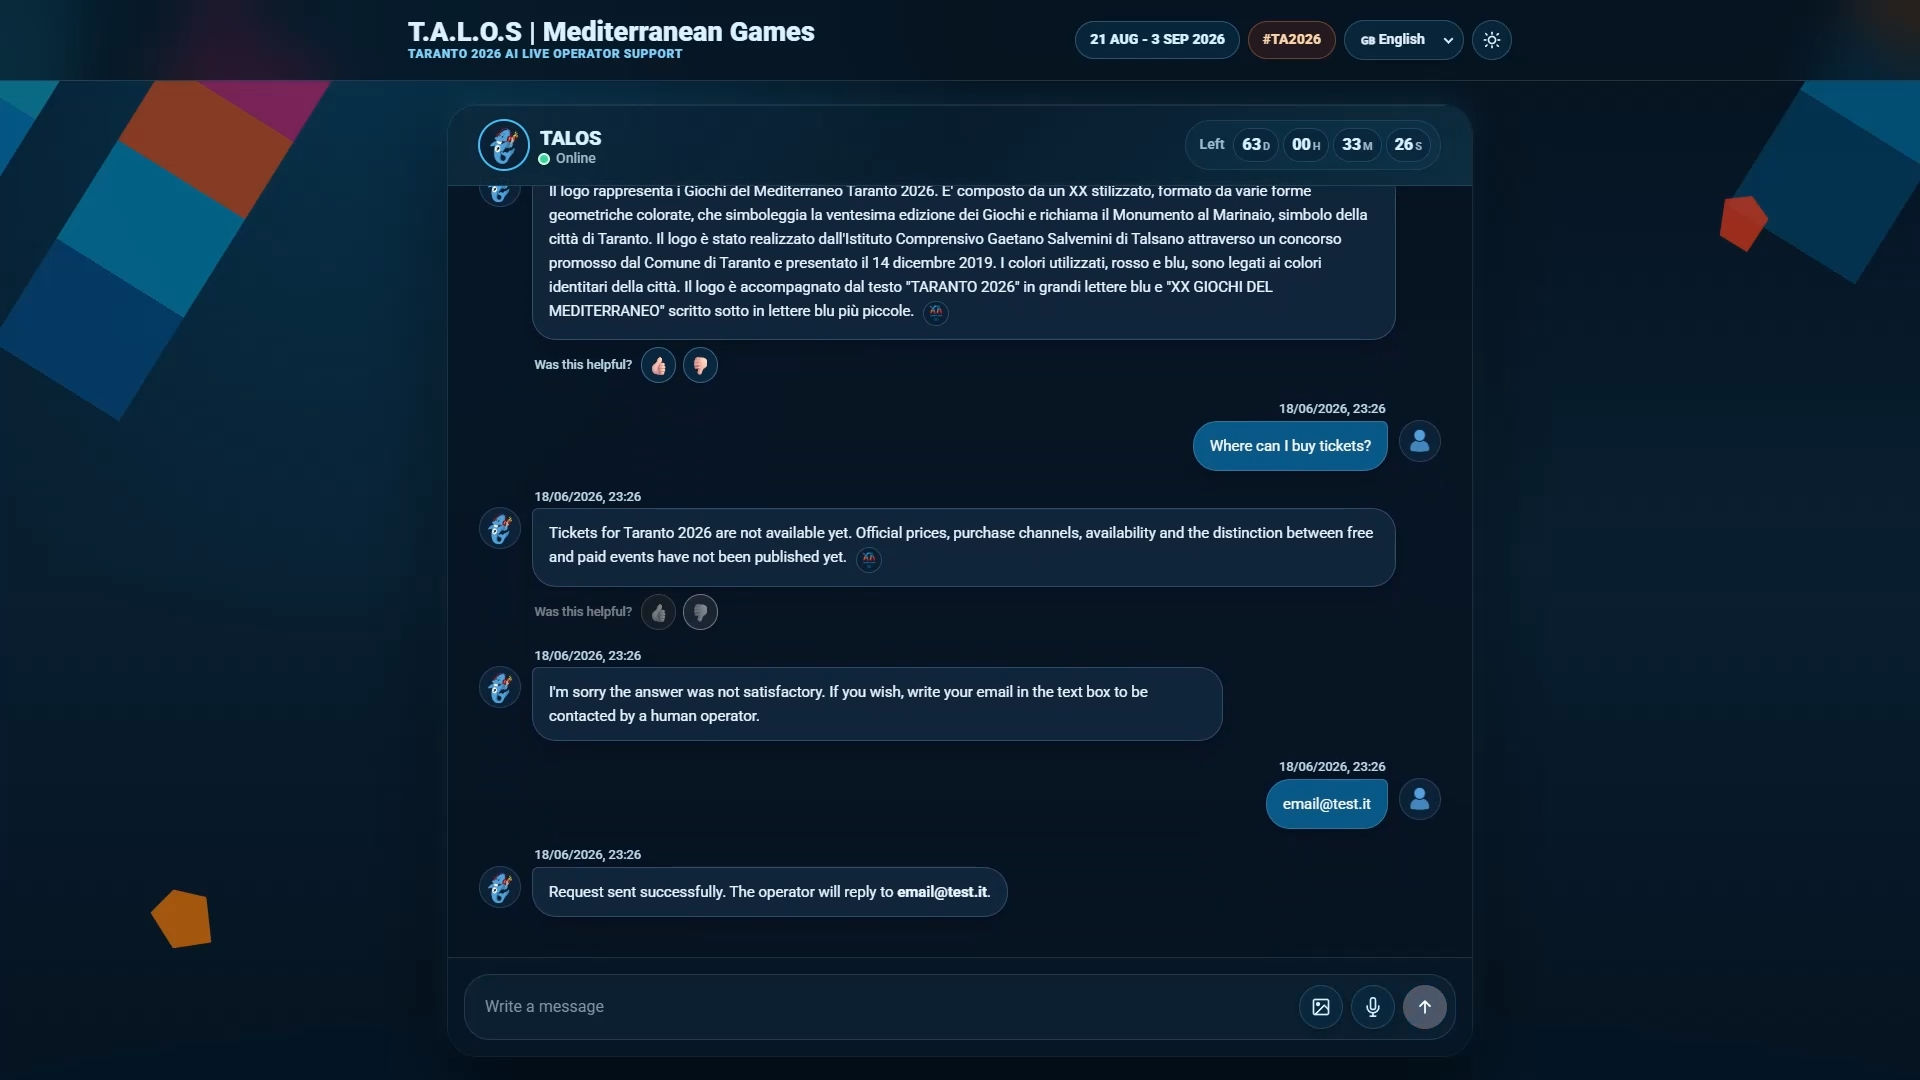
\includegraphics[width=\textwidth]{images/escalation-en-dark.png}
\caption{Escalation verso operatore dopo feedback negativo.}
\label{fig:frontend-escalation}
\end{figure}

La dashboard operatore rappresenta l’area riservata del sistema dedicata alla gestione dei ticket e al customer care. L’accesso avviene tramite una schermata di login, mostrata in Figura~\ref{fig:operator-login}, nella quale l’operatore inserisce le proprie credenziali. Dopo l’autenticazione, il frontend riceve un \textit{JSON Web Token} (JWT) e può accedere alle funzionalità protette della dashboard.

\begin{figure}[H]
\centering
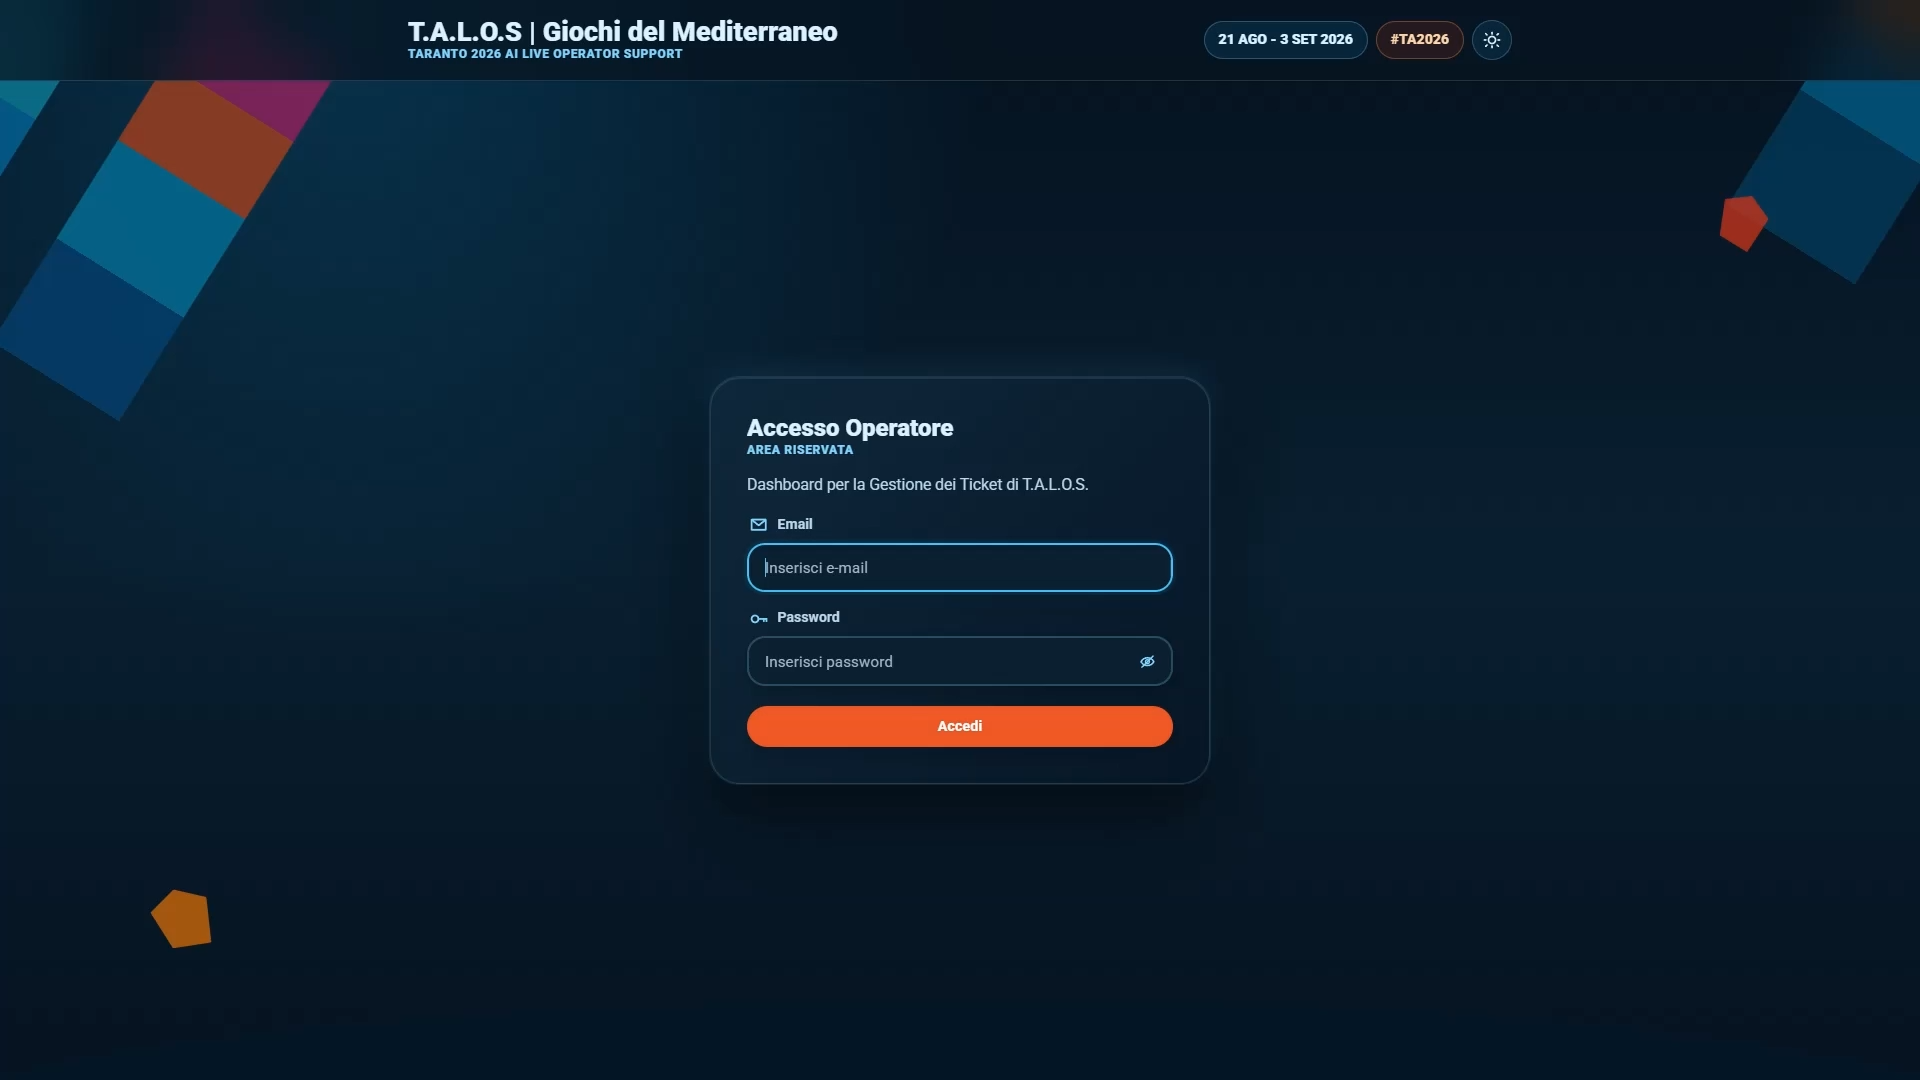
\includegraphics[width=\textwidth]{images/operatore-login.png}
\caption{Schermata di accesso all’area operatore.}
\label{fig:operator-login}
\end{figure}

La dashboard consente all’operatore di visualizzare i ticket generati dal sistema, applicare filtri per stato, ordinare le richieste e selezionare un ticket per consultarne il dettaglio. La Figura~\ref{fig:operator-dashboard} mostra la lista dei ticket in modalità scura, con informazioni sintetiche relative a stato, priorità, dominio, data, e-mail dell’utente e descrizione del problema. Questa vista è pensata per fornire rapidamente una panoramica delle richieste aperte, evitando che l’operatore debba accedere subito al dettaglio di ogni conversazione.

\begin{figure}[H]
\centering
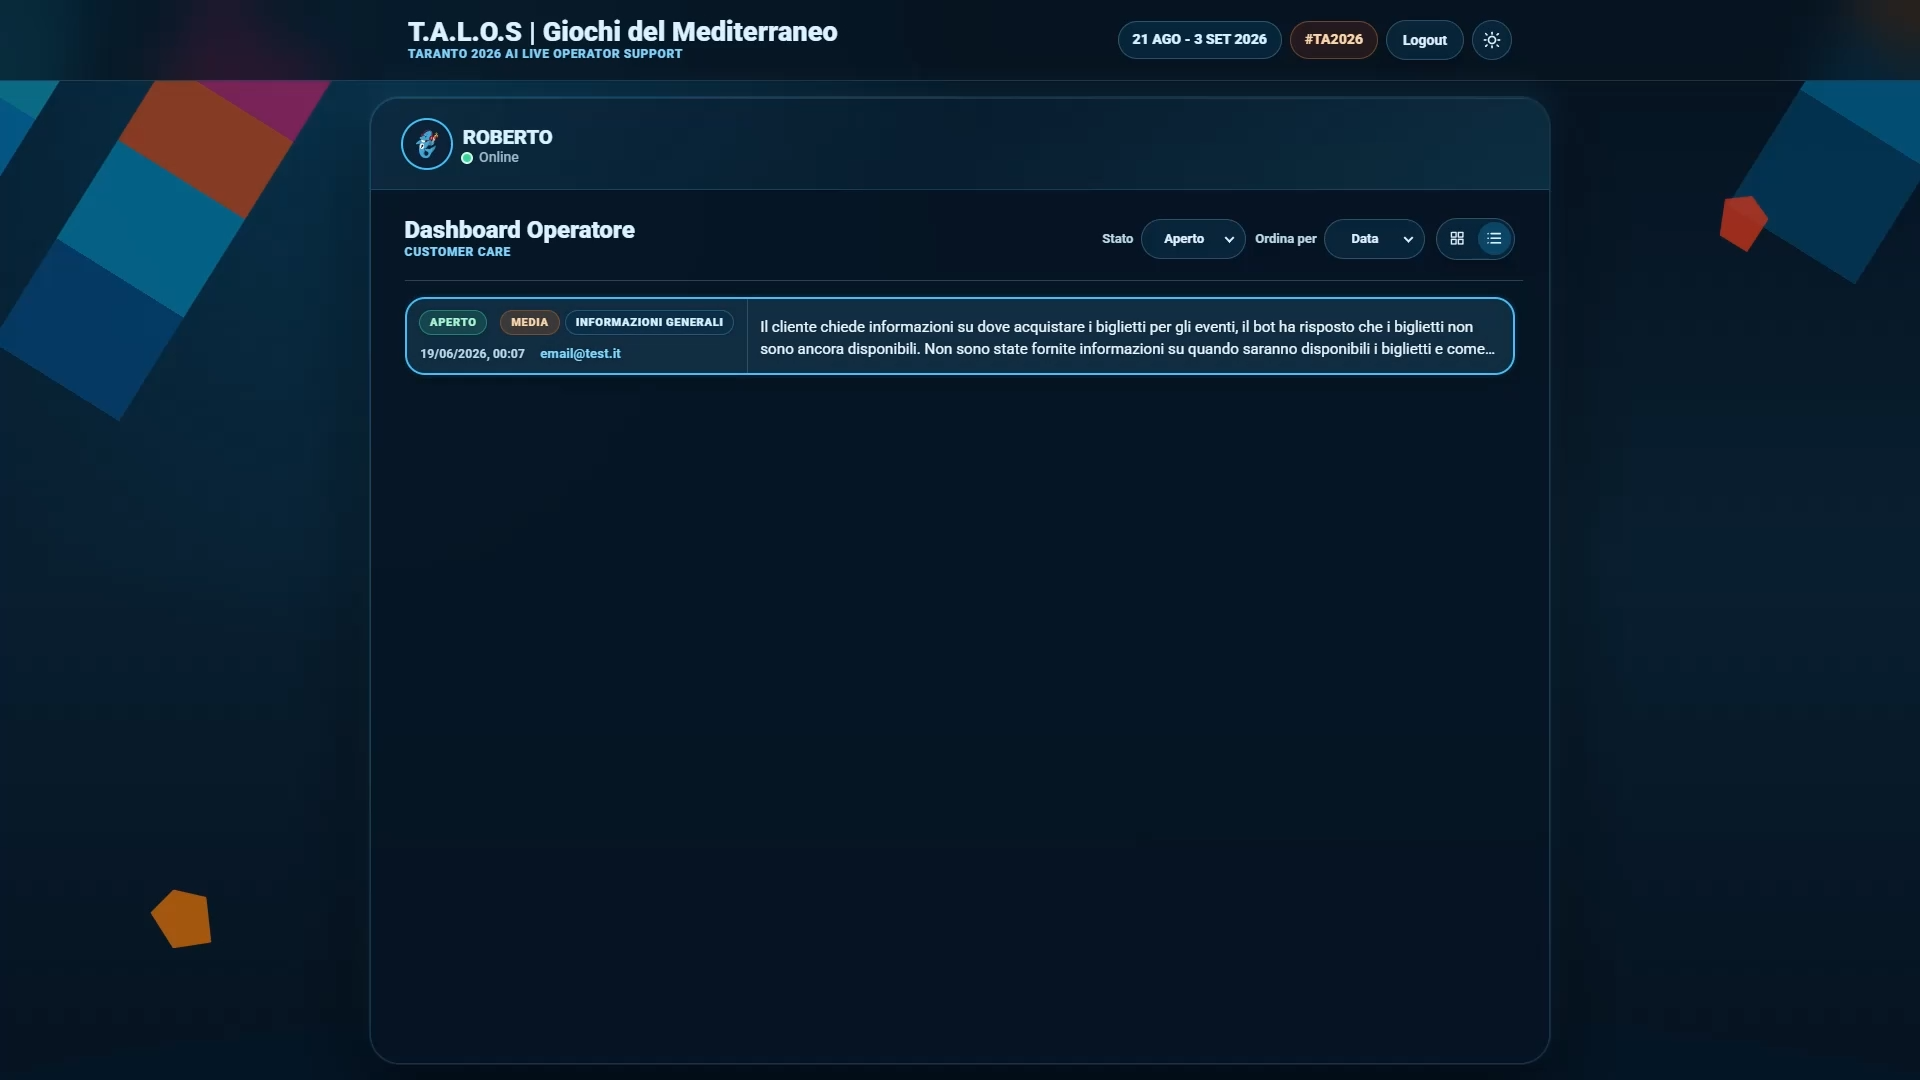
\includegraphics[width=\textwidth]{images/operatore-vista2-dark.png}
\caption{Dashboard operatore con lista dei ticket aperti.}
\label{fig:operator-dashboard}
\end{figure}

La stessa dashboard è disponibile anche con ticket in formato card e in tema chiaro, come mostrato in Figura~\ref{fig:operator-dashboard-light}.

\begin{figure}[H]
\centering
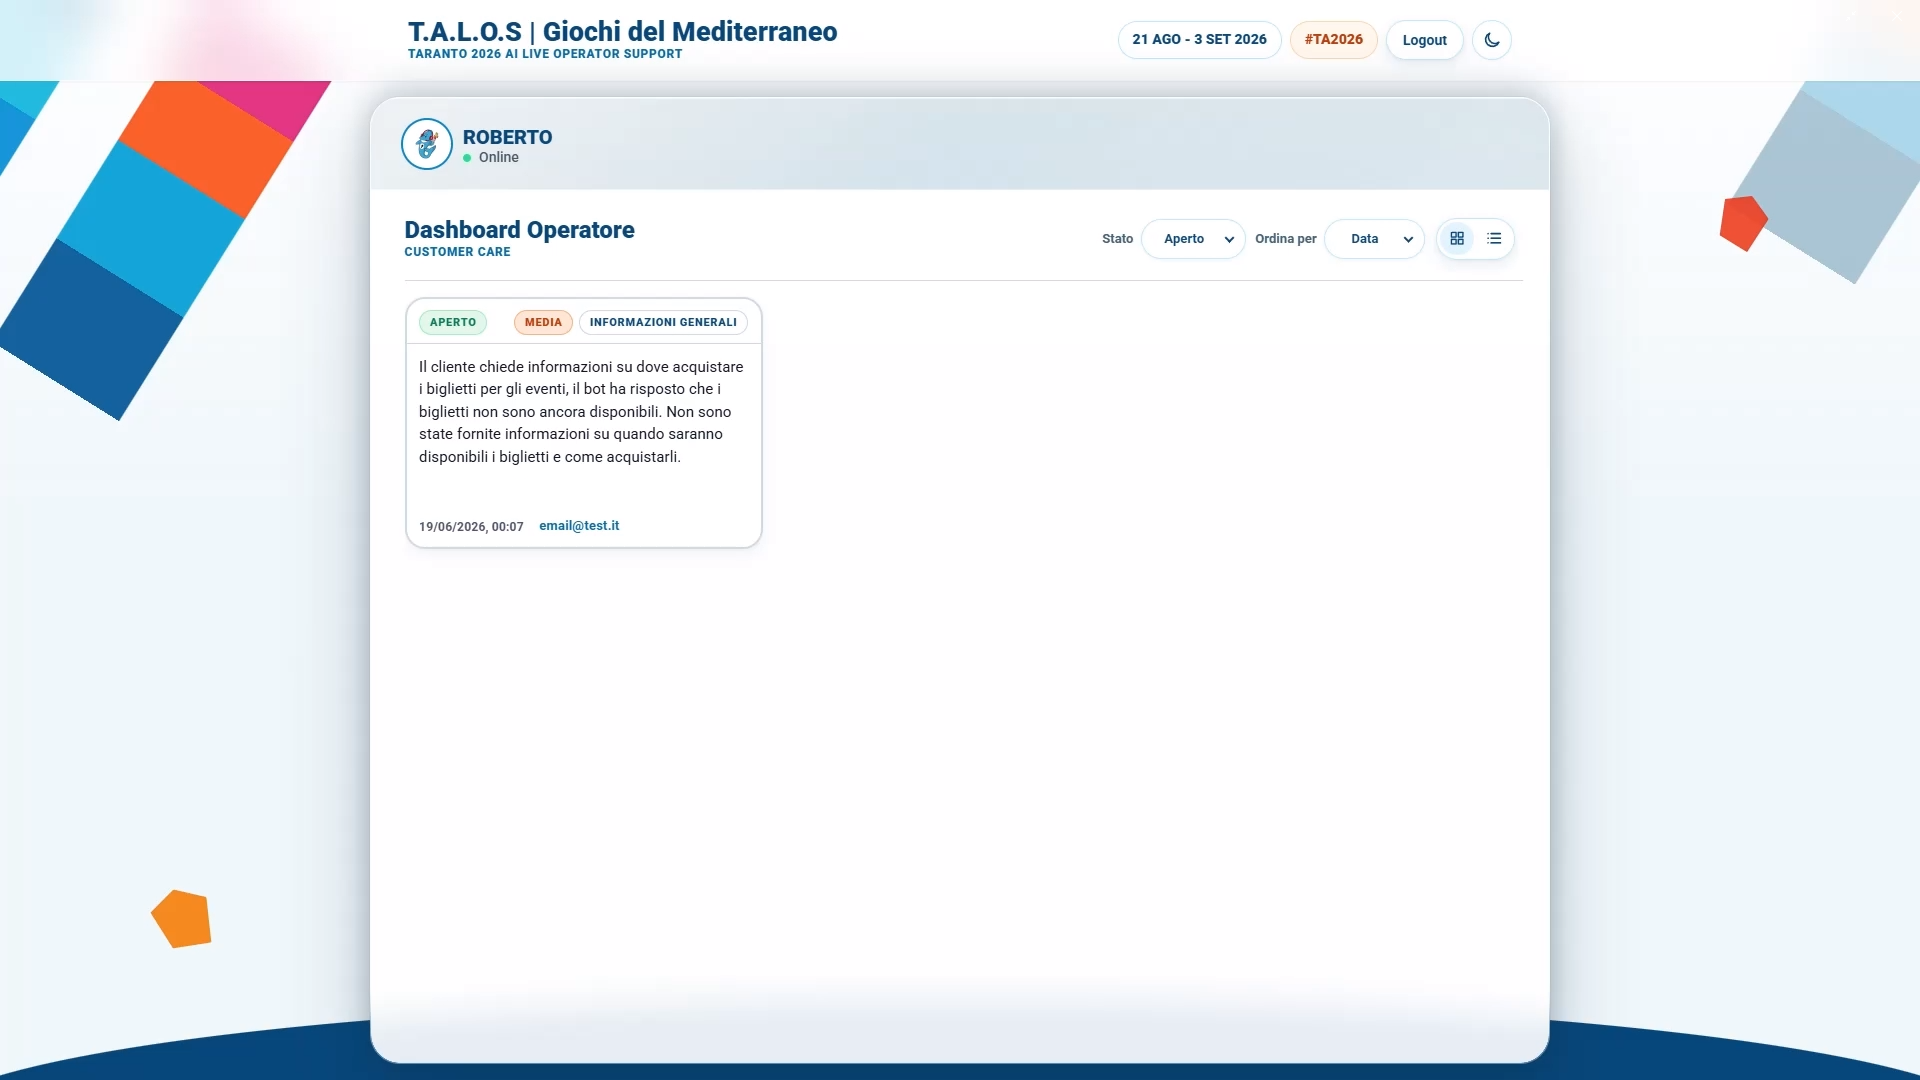
\includegraphics[width=\textwidth]{images/operatore-light.png}
\caption{Dashboard operatore in tema chiaro con card dei ticket aperti.}
\label{fig:operator-dashboard-light}
\end{figure}

Quando l’operatore seleziona un ticket, viene mostrata una vista di dettaglio con le informazioni dettagliate della richiesta. Come si osserva in Figura~\ref{fig:operator-ticket-detail}, il dettaglio include l'intera conversazione, inclusi i messaggi visuali, vocali e le risposte generate dal chatbot. Dalla vista dettagliata è possibile segnare la conversazione come chiusa mediante l'apposito pulsante, terminando il processo di customer care per il ticket corrente.

\begin{figure}[H]
\centering
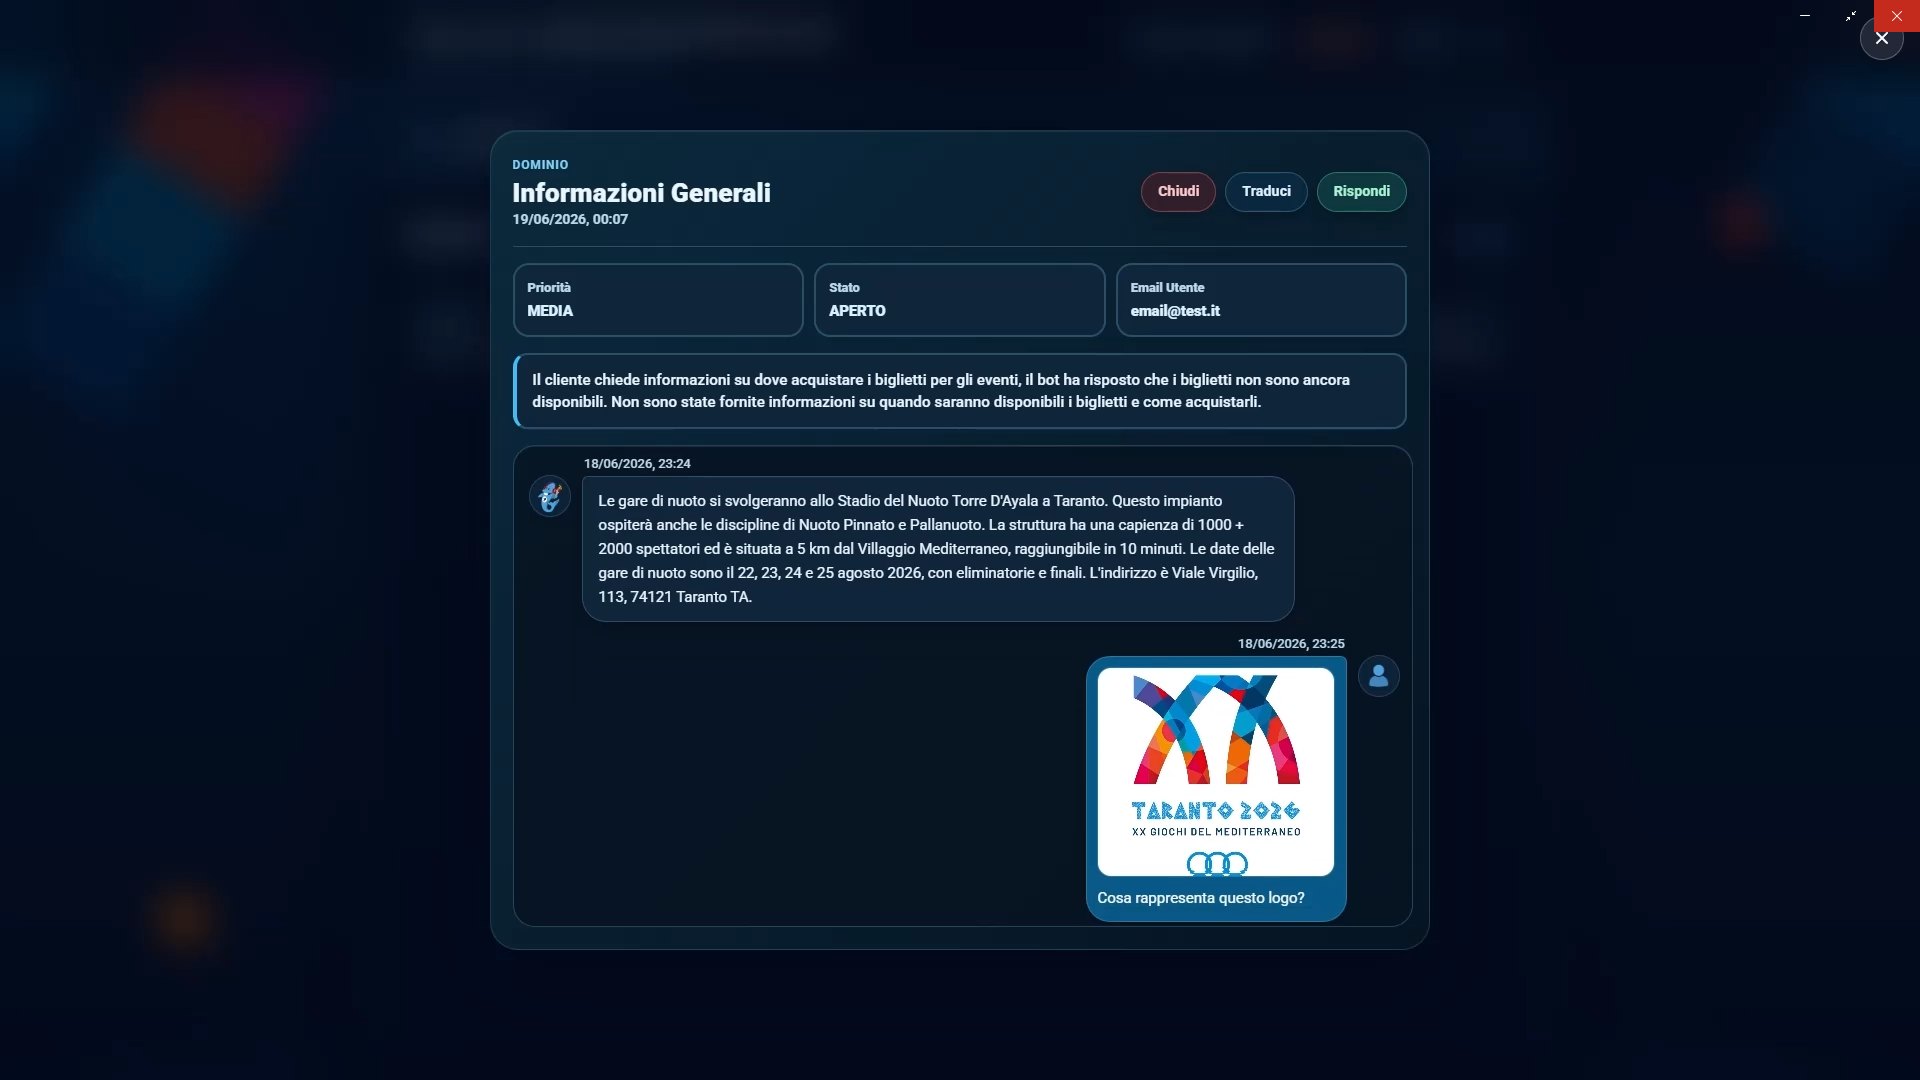
\includegraphics[width=\textwidth]{images/modal-operatore-dark.png}
\caption{Dettaglio di un ticket aperto.}
\label{fig:operator-ticket-detail}
\end{figure}
La dashboard include anche una funzione di traduzione della conversazione. Come mostrato in Figura~\ref{fig:operator-translation}, l’operatore può consultare il contenuto originale oppure richiedere una versione tradotta.
Questa funzionalità è utile perché il chatbot è multilingua e gli utenti possono interagire in lingue diverse dall’italiano, mentre l’operatore può avere la necessità di consultare le richieste in italiano per comodità.

\begin{figure}[H]
\centering
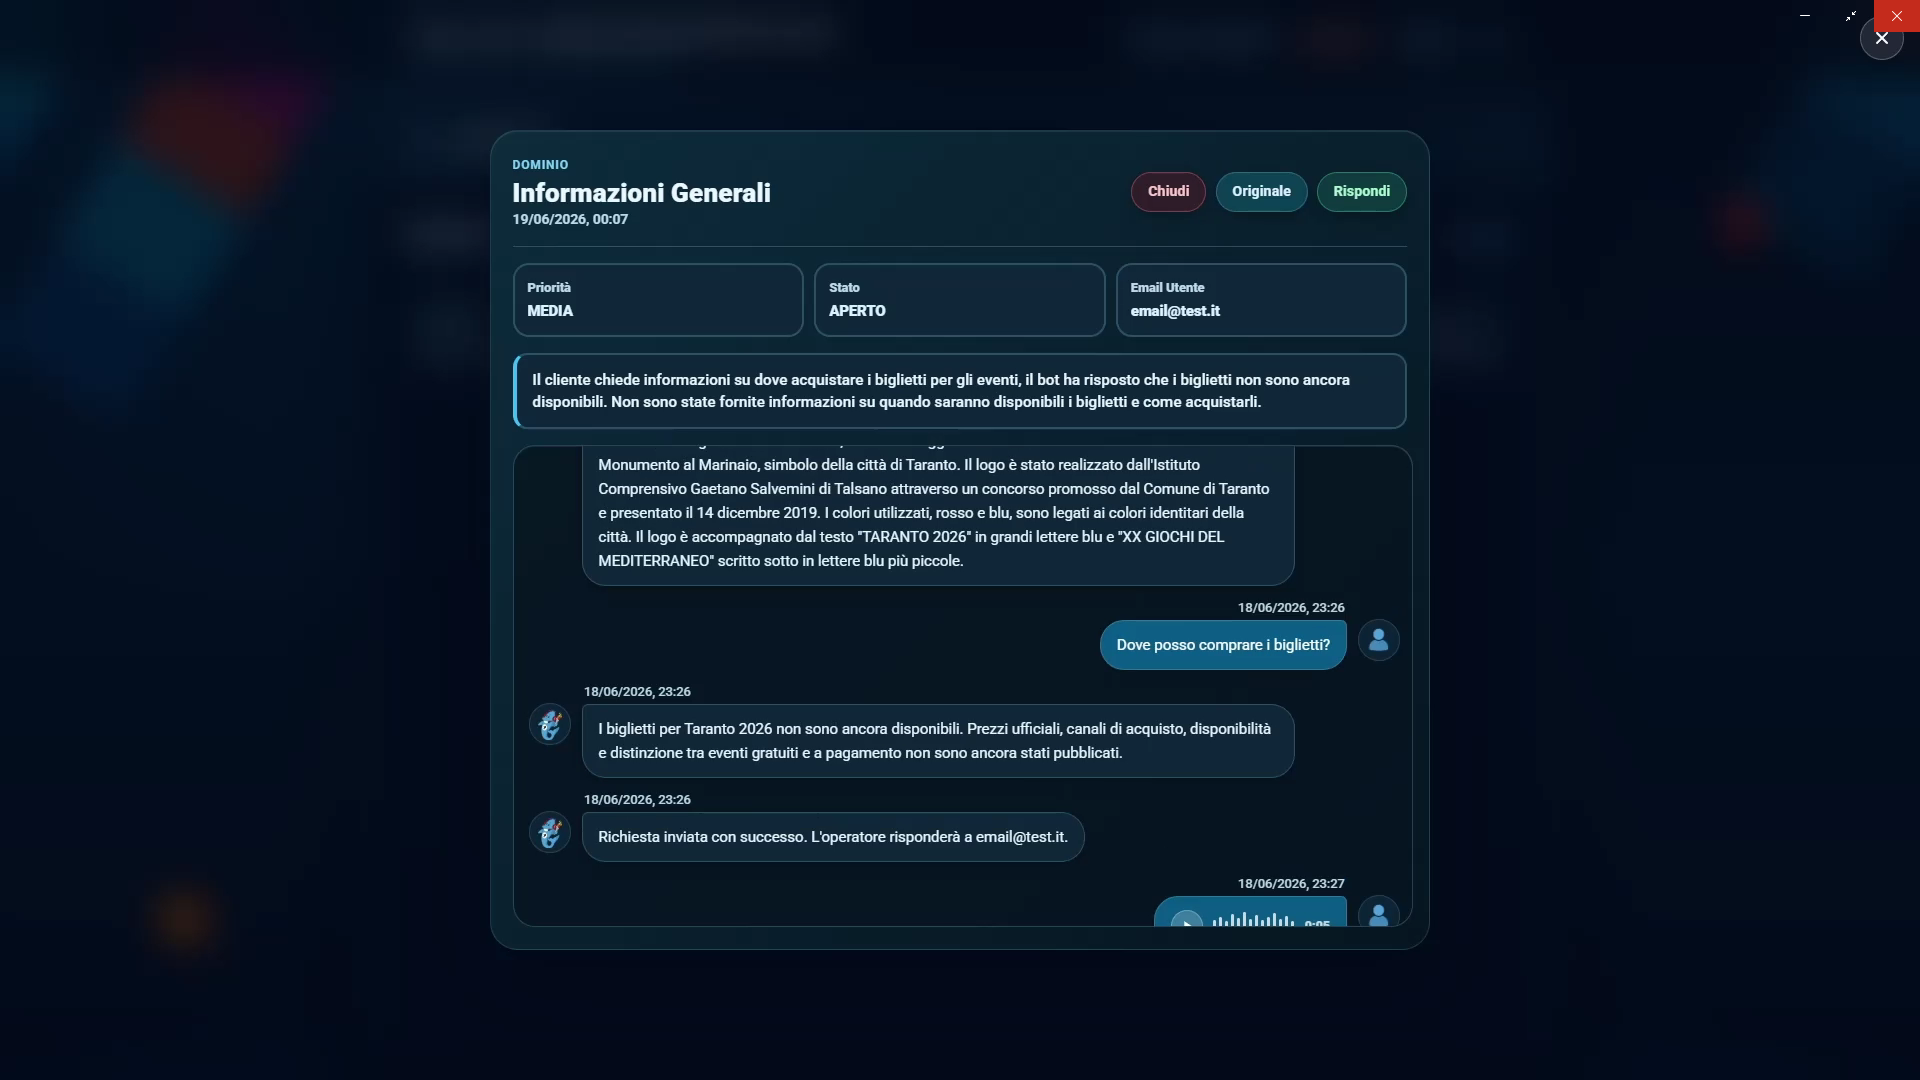
\includegraphics[width=\textwidth]{images/traduzione-modal-dark.png}
\caption{Funzione di traduzione della conversazione nel dettaglio ticket.}
\label{fig:operator-translation}
\end{figure}

Un’ulteriore funzionalità riguarda la generazione di una bozza di risposta e-mail. Il backend produce un oggetto e un corpo del messaggio sulla base del contenuto del ticket e dell'identificativo della conversazione. Il frontend apre quindi una finestra di composizione e-mail tramite \textit{mailto}, come mostrato in Figura~\ref{fig:operator-email}. La bozza non sostituisce il giudizio dell’operatore, ma riduce il tempo necessario per preparare una risposta ordinata e coerente con la richiesta dell’utente.

\begin{figure}[H]
\centering
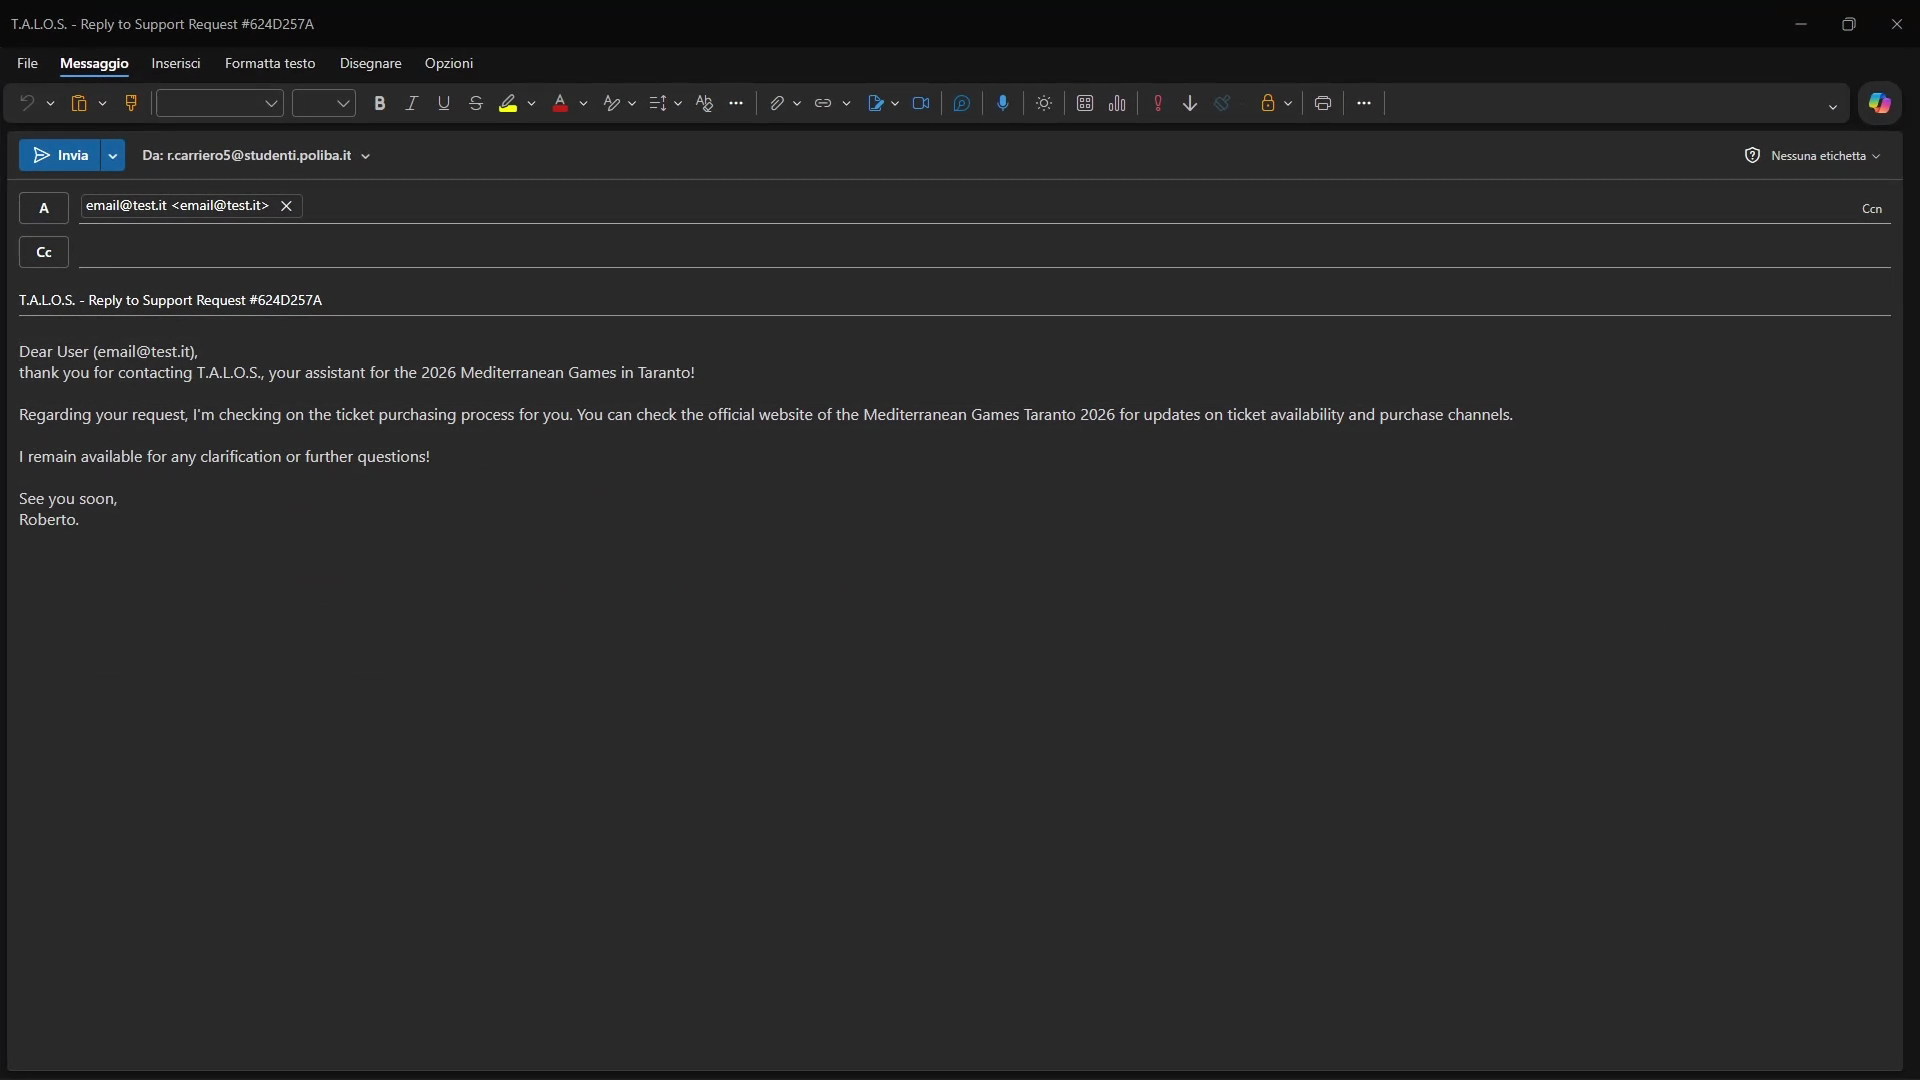
\includegraphics[width=\textwidth]{images/operatore-email.png}
\caption{Bozza e-mail generata a supporto dell’operatore.}
\label{fig:operator-email}
\end{figure}
La pagina di gestione della knowledge base consente a un operatore autorizzato di aggiungere nuovi contenuti informativi tramite interfaccia grafica. La schermata di inserimento, mostrata in Figura~\ref{fig:knowledge-admin}, permette di creare un nuovo record indicando titolo, fonte, tipo, dominio e documento. Il campo documento rappresenta il contenuto principale che verrà indicizzato e recuperato dal chatbot. A seconda della tipologia e del dominio selezionato vengono abilitati campi aggiuntivi per l'inserimento delle coordinate geografiche e dell'indirizzo completo.

\begin{figure}[H]
\centering
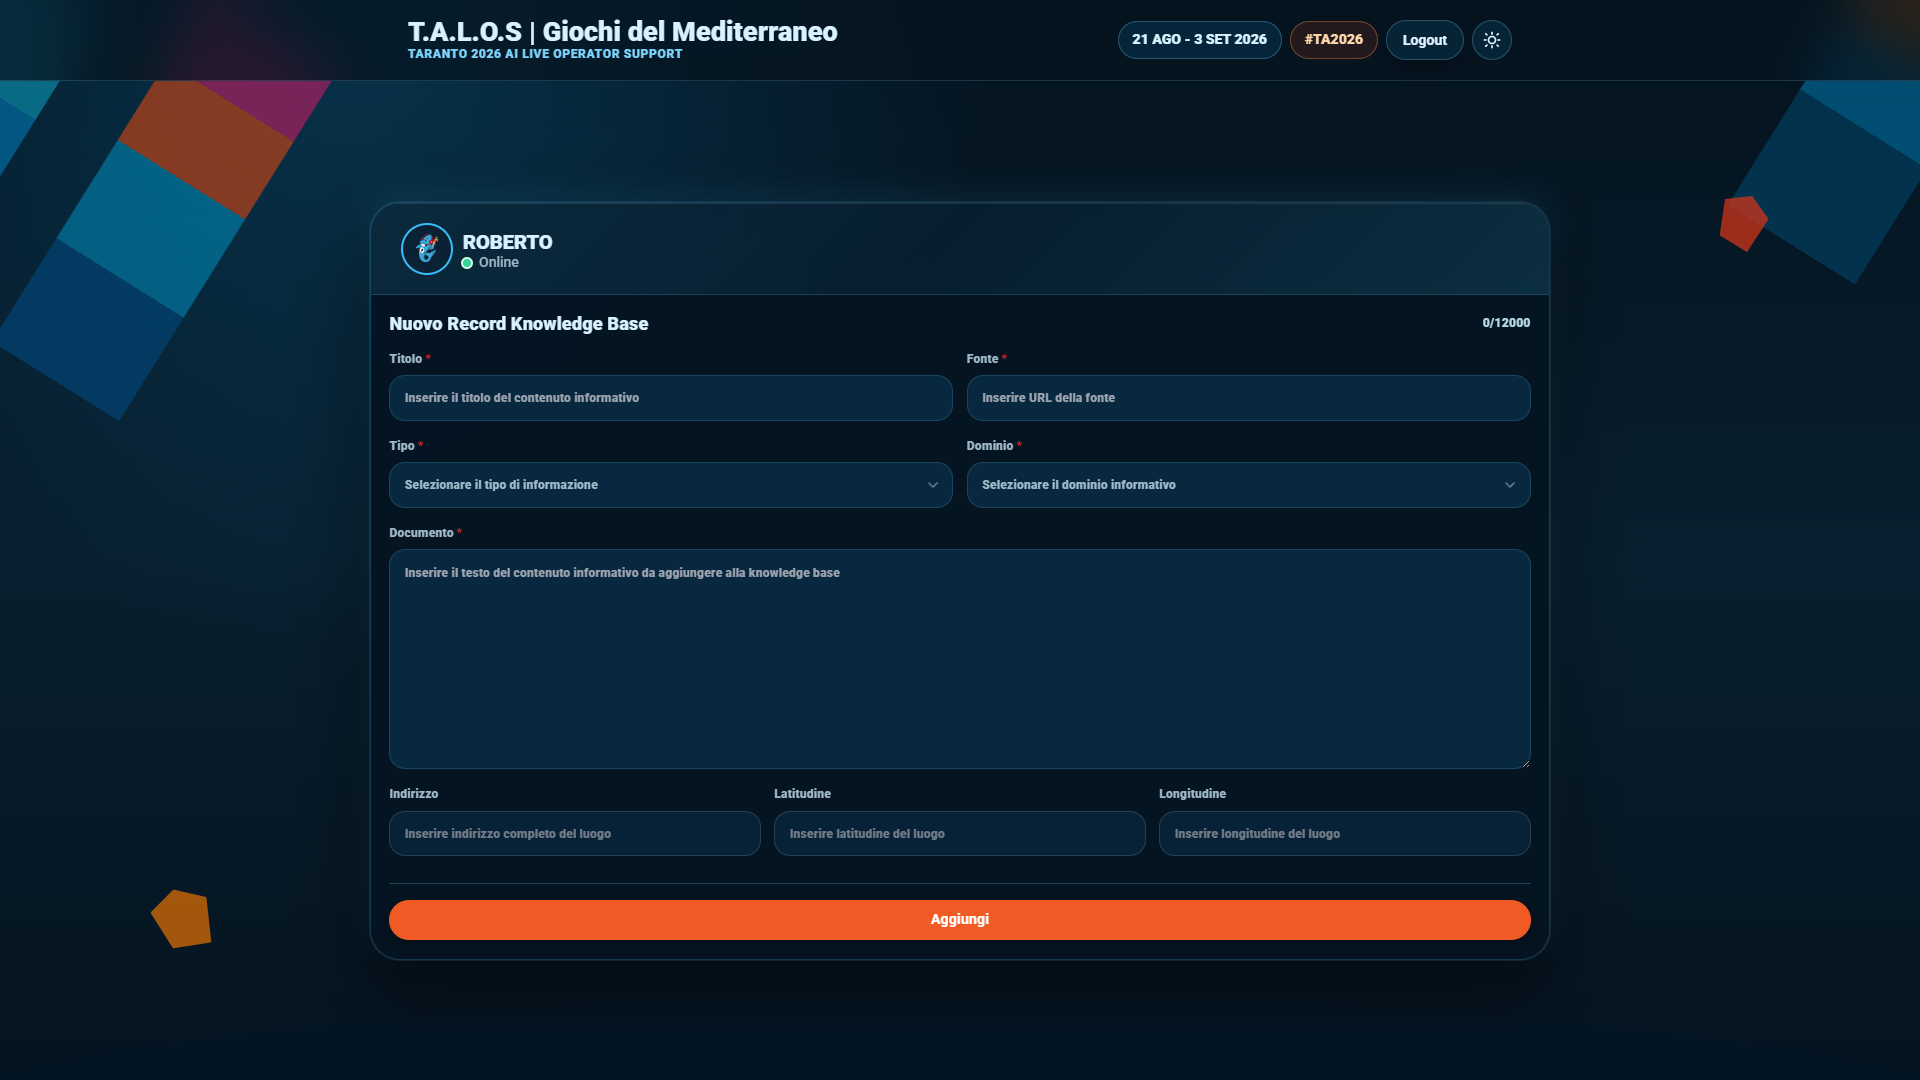
\includegraphics[width=\textwidth]{images/ingest-dark.png}
\caption{Interfaccia grafica per l'aggiornamento della base di conoscenza.}
\label{fig:knowledge-admin}
\end{figure}
Dopo l’invio del form, il backend valida il \textit{payload}, genera l’identificativo del record, prepara i metadati, aggiunge il contenuto al file JSONL e lo indicizza in ChromaDB. In questo modo, il nuovo contenuto diventa subito recuperabile dalla pipeline RAG nelle conversazioni successive, senza necessità di riavviare il sistema.

La progettazione responsive è stata verificata anche su smartphone, utilizzando l’accesso HTTPS generato tramite Cloudflare Tunnel. Questo test è cruciale perché il sistema è pensato soprattutto per utenti che durante l’evento potrebbero accedere al servizio direttamente da telefono, ad esempio tramite link, QR code o \textit{Progressive Web App }(PWA) installata. In modalità mobile, l’interfaccia mantiene le stesse funzionalità principali della versione desktop, ma riorganizza gli elementi per adattarli allo spazio ridotto dello schermo.

Come mostrato in Figura~\ref{fig:frontend-mobile}, la versione mobile conserva le tre interfacce principali del sistema per chatbot, dashboard operatore e gestione knowledge base. Nel chatbot, l’header mantiene il logo, il nome del sistema e il countdown, mentre l’area della conversazione viene organizzata in una card verticale più compatta. I controlli per lingua, tema, e input multimodali restano disponibili, ma vengono disposti in modo più adatto all’interazione touch.

Anche la dashboard operatore viene adattata al formato verticale. Rispetto alla versione desktop, in cui filtri e ordinamento possono essere distribuiti orizzontalmente, nella versione mobile gli elementi vengono impilati e resi più grandi, così da essere leggibili e selezionabili.

La pagina di aggiornamento della base di conoscenza segue la stessa logica responsive. Nella versione desktop alcuni campi del form possono essere affiancati, mentre nella vista mobile vengono disposti in sequenza verticale per rendere più semplice l’inserimento dei dati.

\begin{figure}[H]
\centering
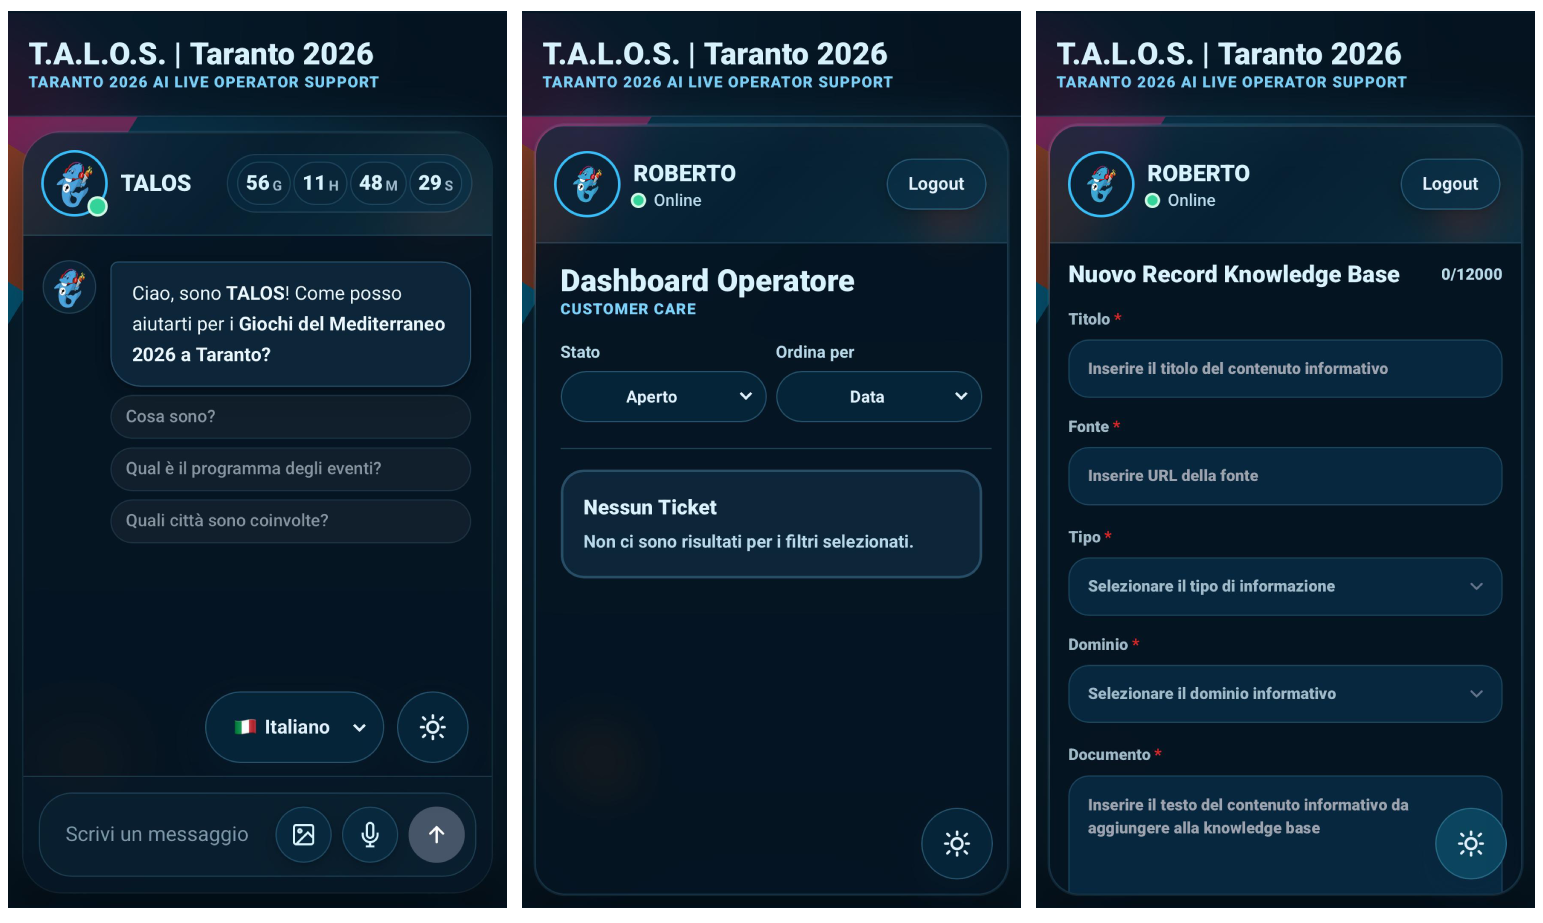
\includegraphics[width=\textwidth]{images/mobile.png}
\caption{Interfacce principali del sistema responsive su mobile.}
\label{fig:frontend-mobile}
\end{figure}

\section{Deployment}

Il file \textit{docker-compose.yml} definisce i container principali del progetto. I servizi comunicano tra loro attraverso la rete Docker interna \textit{talos-network}, utilizzando i nomi dei container come host. In questo modo, il backend può raggiungere ChromaDB tramite \textit{vector-db}, PostgreSQL tramite \textit{database} e Ollama tramite \textit{llm}, senza dover dipendere da indirizzi IP locali. Per la persistenza dei dati, Docker Compose definisce volumi dedicati per PostgreSQL, ChromaDB, pgAdmin, modelli Ollama e upload.

Il progetto può essere avviato in due modalità. La modalità completa include anche Ollama e il servizio \textit{llm-init}, che si occupa del download automatico dei modelli configurati, come il modello testuale e il modello vision. Questa modalità è più autonoma, perché consente di utilizzare modelli locali, ma può richiedere GPU NVIDIA e spazio disco sufficiente per i pesi dei modelli. La modalità \textit{lite}, invece, è pensata per scenari in cui è disponibile una chiave Groq e non si vuole eseguire il modello locale.

Per semplificare l’avvio su \textit{Windows} e \textit{macOS} sono stati predisposti gli script \textit{run.bat} e \textit{run.sh}. Entrambi accettano le modalità \textit{full} e \textit{lite}, inizializzano i servizi necessari, attendono che il database e il backend siano attivi e recuperano automaticamente il link HTTPS generato da Cloudflare Tunnel. Essi sono stati introdotti per rendere il frontend accessibile anche da dispositivi mobili in un contesto sicuro. Questo è necessario perché alcune funzionalità, come l’uso del microfono o l’installazione della PWA, richiedono una connessione HTTPS per funzionare correttamente sui browser moderni. Il link gratuito \textit{trycloudflare.com} cambia a ogni riavvio del tunnel e risulta quindi adeguato per test e demo, ma non per un ambiente di produzione.

Il riepilogo dei servizi containerizzati è riportato in Tabella~\ref{tab:docker-services}, mentre il dettaglio della configurazione Docker Compose è riportato in Appendice~\ref{app:docker-compose}.

\begin{table}[H]
\centering
\caption{Servizi Docker presenti nel progetto.}
\label{tab:docker-services}
{\small
\begin{tabular}{p{0.18\textwidth}p{0.17\textwidth}p{0.12\textwidth}p{0.41\textwidth}}
\toprule
\textbf{Servizio} & \textbf{Tecnologia} & \textbf{Porta} & \textbf{Responsabilità}\\
\midrule
\textbf{frontend}& React/Vite & 5173 & Chat, PWA, dashboard operatore e interfaccia di gestione knowledge base.\\
\textbf{backend}& FastAPI & 8000 & API, orchestrazione RAG e modelli AI, ticketing.\\
\textbf{vector-db}& ChromaDB & 8001 & Indicizzazione e ricerca semantica dei record della knowledge base.\\
\textbf{database}& PostgreSQL 16 & 5433 & Persistenza di conversazioni, messaggi, operatori e ticket.\\
\textbf{pgadmin}& pgAdmin4 & 5050 & Ispezione visuale del database durante lo sviluppo.\\
\textbf{llm}& Ollama & 11434 & Esecuzione locale dei modelli AI.\\
\textbf{cloudflared}& Cloudflare Tunnel & \textemdash{} & Esposizione HTTPS temporanea per demo.\\
\bottomrule
\end{tabular}
}
\end{table}
\chapter{Risultati e conclusioni}

Al termine della fase di sviluppo è stato eseguito un test automatizzato con l’obiettivo di misurare la qualità complessiva del sistema e raccogliere metriche quantitative riconducibili ai principali KPI individuati e descritti di seguito. Questa sezione esamina inoltre i limiti dell'implementazione corrente e le possibili linee di sviluppo futuro, ponendo le basi per le riflessioni conclusive.

\section{Testing automatizzato}

La valutazione del sistema è stata predisposta tramite uno script automatizzato contenuto nella cartella \textit{eval}. In particolare, il file \textit{run\_kpi\_eval.py} esegue una serie di test simulati a partire dal dataset \textit{test\_dataset.jsonl} e produce un riepilogo dei risultati nel file \textit{eval/outputs/results.csv}.

Il dataset utilizzato per il testing non rappresenta interazioni reali raccolte da utenti esterni, ma un insieme di casi d’esempio costruiti per verificare il comportamento del sistema rispetto a domande il più possibile vicine a quelle che potrebbero essere formulate dagli utenti finali. I casi sono stati definiti cercando di mantenere eterogeneità nei contenuti, nei domini informativi e nelle possibili modalità di richiesta. Di conseguenza, i risultati ottenuti misurano la qualità del sistema in un ambiente controllato, ma non certificano in modo definitivo le prestazioni in uno scenario reale, caratterizzato da utenti esterni, formulazioni imprevedibili e richieste ambigue.

Il dataset di test contiene \textit{130} casi testuali. Le domande coprono diversi domini informativi, tra cui informazioni generali, venue, calendario, ticketing, volontariato e accessibilità. La maggior parte dei casi è in italiano, ma sono presenti anche esempi in inglese, spagnolo, francese e arabo, così da verificare il comportamento multilingua del sistema. Per ogni caso vengono specificati l’identificativo del test, la modalità, il messaggio, la lingua, il dominio atteso, i documenti rilevanti attesi, il feedback simulato e, in alcuni casi, l’eventuale apertura di un ticket.

Il runner esegue prima una fase di validazione del dataset. In questa fase controlla che ogni caso abbia un identificativo, che non ci siano duplicati, che la modalità sia ammessa e che i campi richiesti siano coerenti con il tipo di test. Ad esempio, un caso testuale deve avere un messaggio, mentre eventuali casi audio o immagine dovrebbero indicare un file associato.

I KPI individuati possono essere organizzati in tre macroaree. La prima è la qualità informativa, misurata da \textit{Domain Accuracy}, \textit{Recall@5}, \textit{Precision@5}, \textit{Mean Reciprocal Rank} (MRR) e \textit{Source Coverage Rate}. La seconda è la performance tecnica, misurata da \textit{Average Latency}, \textit{p95 Latency} ed \textit{Error Rate}. La terza è l’impatto operativo, misurato da \textit{Escalation Rate}, \textit{Containment Rate} e \textit{Feedback Score}. La qualità informativa dipende dalla knowledge base e dal retrieval, la qualità conversazionale dipende dal frontend, dal backend e dal modello linguistico, mentre la dimensione operativa dipende da ticket, dashboard e feedback.

Per misurare la qualità informativa, il runner importa direttamente le funzioni di query planning e retrieval del backend, costruisce il piano della richiesta, interroga il servizio RAG e confronta i documenti recuperati con quelli attesi nel dataset. Per quanto riguarda la performance tecnica, invece, il runner invia una richiesta all’endpoint \textit{/api/chat}, costruendo un \textit{session\_id} specifico. Il backend elabora la richiesta come avverrebbe in una normale conversazione, genera la risposta, restituisce eventuali fonti, salva i messaggi e produce le informazioni necessarie per feedback e ticket. Il runner misura quindi latenza, successo della chiamata, presenza di errori, copertura delle fonti ed eventuale comportamento di escalation.

Il flusso prevede anche la possibilità di pubblicare feedback e ticket simulati. Se l’opzione è abilitata, il runner invia il feedback all’endpoint \textit{/api/messages/message\_id/feedback}. Nei casi predisposti per l’escalation, invia inoltre una richiesta all’endpoint \textit{/api/tickets}.

Il runner confronta lo stato del database e calcola metriche come escalation rate cumulativo, containment rate cumulativo, feedback score e delta dei nuovi ticket rispetto alle nuove conversazioni create durante la run. Questa scelta collega la valutazione automatica ai dati realmente salvati dal sistema.

Il file \textit{results.csv} generato dal runner contiene un riepilogo aggregato dei risultati ottenuti. Ogni riga del \textit{CSV} riporta il nome del KPI, una breve descrizione, il valore calcolato e l’unità di misura.

\section{Valutazione metriche e KPI}

Pur in assenza di un \textit{Service Level Agreement} (SLA) formalmente definito, i risultati emersi dal file CSV evidenziano comunque un comportamento complessivamente positivo del sistema, almeno con riferimento a uno scenario controllato basato su richieste utente di base. Le metriche di qualità informativa indicano che il sistema riesce, nella maggior parte dei casi, a classificare correttamente il dominio della richiesta e a recuperare documenti pertinenti dalla knowledge base. Le metriche operative evidenziano invece una buona capacità di contenere le richieste informative senza ricorrere sistematicamente all’intervento dell’operatore umano.

La Tabella~\ref{tab:kpi-results} riporta i principali KPI registrati nel file \textit{results.csv}.

\begingroup
\small
\begin{longtable}{p{0.24\textwidth}p{0.18\textwidth}p{0.48\textwidth}}
\caption{Risultati ottenuti dal test automatizzato.}
\label{tab:kpi-results}\tabularnewline
\toprule
\textbf{KPI} & \textbf{Descrizione} & \textbf{Interpretazione}\tabularnewline
\midrule
\textbf{Domain Accuracy} & 92.62\% & Il sistema classifica correttamente la maggior parte dei domini informativi delle domande di test.\tabularnewline
\textbf{Recall@5} & 79.51\% & In circa quattro casi su cinque almeno un documento rilevante compare tra i primi cinque risultati recuperati.\tabularnewline
\textbf{Precision@5} & 74.75\% & La quota media di documenti pertinenti nei primi cinque risultati è elevata, indicando un retrieval complessivamente selettivo.\tabularnewline
\textbf{MRR} & 0.7204 & Il primo documento corretto tende a comparire in posizione alta quando viene recuperato.\tabularnewline
\textbf{Source Coverage Rate} & 79.07\% & La maggior parte delle risposte valide contiene almeno una fonte recuperata dalla knowledge base.\tabularnewline
\textbf{Average Latency} & 5.65 s & Il tempo medio end-to-end è basso.\tabularnewline
\textbf{p95 Latency} & 10.92 s & Il 95\% delle richieste rientra entro circa 11 secondi.\tabularnewline
\textbf{Error Rate} & 0.77\% & Le richieste fallite sono molto poche rispetto al totale dei casi valutati.\tabularnewline
\textbf{Escalation Rate} & 6.20\% & Una quota limitata di conversazioni simulate viene trasferita o trasformata in ticket operatore.\tabularnewline
\textbf{Containment Rate} & 93.80\% & La maggior parte delle richieste simulate viene gestita senza intervento umano.\tabularnewline
\textbf{Feedback Score} & 92.73\% & I messaggi valutati nel database risultano prevalentemente soddisfacenti.\tabularnewline
\bottomrule
\end{longtable}
\endgroup

La Domain Accuracy del 92.62\% è uno dei risultati più solidi. Indica che il sistema riesce a riconoscere correttamente il dominio della richiesta nella maggior parte dei casi. Questo risultato è importante perché il dominio influenza il retrieval e la costruzione della risposta. Se il dominio è errato, il sistema rischia di interrogare documenti meno pertinenti e di fornire un contesto meno adatto al modello linguistico.

Recall@5 pari al 79.51\% indica che, nella maggior parte dei casi, almeno un documento rilevante entra tra i primi cinque risultati recuperati. In un sistema RAG questo aspetto è fondamentale, perché il modello linguistico può generare una risposta fondata solo se il documento corretto entra nel contesto. Quando il documento rilevante non viene recuperato, anche un buon modello linguistico può rispondere in modo incompleto o troppo generico.

Precision@5 pari al 74.75\% è un risultato positivo, perché indica che una parte consistente dei primi cinque documenti recuperati è pertinente rispetto alla domanda.

Con un MRR del 72\%, i dati confermano che i documenti pertinenti recuperati compaiono tipicamente nei primi risultati. Questo è rilevante perché i primi documenti influenzano maggiormente il prompt e quindi la risposta finale. Un MRR vicino a 1 indicherebbe che il primo risultato è quasi sempre corretto.

Il Source Coverage Rate del 79.07\% indica che la maggior parte delle risposte valide viene accompagnata da almeno una fonte. Questo dato è importante in un sistema informativo, perché le fonti aumentano tracciabilità e fiducia.

Il tempo medio di risposta è di circa 6 secondi, mentre il p95 arriva a circa 11 secondi. Questi valori sono accettabili per un servizio conversazionale in tempo reale, dove l’utente si aspetta risposte quasi immediate.

L’Error Rate pari allo 0.77\% è molto basso e indica che il sistema fallisce raramente durante la valutazione. Questo dato è particolarmente significativo, poiché riflette la buona affidabilità del flusso applicativo nel suo complesso.

Dal punto di vista operativo, Escalation Rate e Containment Rate devono essere letti insieme. L’Escalation Rate del 6.20\% indica che una parte limitata delle conversazioni simulate viene trasferita o trasformata in ticket. Il Containment Rate del 93.80\% indica invece che la maggior parte delle richieste di test viene gestita senza intervento umano.

Il Feedback Score del 92.73\% è positivo e rispecchia la soddisfazione degli utenti in riferimento all'intero flusso di utilizzo del sistema.

\section{Limiti e sviluppi futuri}

Lo stato attuale del progetto, pur mostrando un pieno funzionamento del prototipo, presenta alcuni limiti e criticità che devono essere considerati in vista di una possibile evoluzione verso un utilizzo reale.

Un primo limite riguarda la natura simulata del benchmark. Il dataset utilizzato rende la valutazione ripetibile e controllabile, ma non può rappresentare pienamente il comportamento degli utenti che potrebbero utilizzare l’applicazione durante l’evento. In un contesto operativo reale, è opportuno considerare che le richieste degli utenti possono assumere forme notevolmente più complesse e articolate rispetto a uno scenario sperimentale. Esse possono infatti contenere errori ortografici o sintattici, ambiguità semantiche, formulazioni incomplete o ellittiche, nonché riferimenti impliciti a contesti non dichiarati. Tali fattori introducono un livello di variabilità e incertezza che mette alla prova le capacità di comprensione e adattamento dell'agente AI, richiedendo soluzioni robuste in grado di gestire la naturale imprecisione del linguaggio umano senza compromettere l'affidabilità della risposta.

Un secondo limite riguarda la valutazione multimodale. Il sistema supporta input audio e immagini, ma queste modalità non sono ancora incluse nel benchmark automatico. Per una valutazione più completa sarebbe necessario costruire un dataset dedicato, composto da file audio, immagini reali, screenshot, foto sfocate e contenuti acquisiti in condizioni non ideali. Sarebbero inoltre necessarie metriche specifiche per valutare la qualità della trascrizione audio, dell’OCR e della descrizione visuale.

Un ulteriore limite riguarda la gestione delle informazioni dinamiche. La knowledge base è adatta a contenere informazioni relativamente stabili, ma non può sostituire fonti live o dati soggetti ad aggiornamenti frequenti, che richiederebbero integrazioni con API ufficiali o sorgenti aggiornate automaticamente. Quando i dati non sono disponibili, il sistema deve adottare un comportamento chiaro e prevedibile: segnalare all'utente l'indisponibilità dell'informazione, senza alcun tentativo di supplire con risposte generate in assenza di fonti. In termini operativi, questo significa rispondere con un messaggio standardizzato che spieghi i motivi della mancata risposta, evitando qualsiasi forma di "invenzione" o di completamento speculativo e orientando eventualmente l'utente verso canali alternativi (operatore umano, documentazione, FAQ).
Questa policy non è un limite, ma una garanzia, in quanto tutela la qualità del servizio e la credibilità del sistema, evitando che un errore informativo si trasformi in un danno per l'utente o per l'azienda.

Anche l'aspetto della sicurezza offre margini di intervento e ottimizzazione. Il sistema include già alcuni elementi di sicurezza di base, ma una versione di produzione richiederebbe interventi più strutturati, come la gestione dei ruoli, l’uso stabile di HTTPS, una configurazione più restrittiva del \textit{CORS}, meccanismi di \textit{rate limiting}, monitoraggio, backup, protezione degli upload e gestione conforme dei dati personali nel rispetto del GDPR e delle procedure tipiche di un servizio di customer care.

Un possibile sviluppo riguarda lo smistamento dei ticket tra più operatori. Nello stato attuale, la dashboard dimostra il passaggio dalla chat al ticket, ma non implementa ancora un sistema completo di assegnazione automatica. In un contesto operativo reale, la distribuzione dei ticket deve essere governata da una pluralità di criteri interconnessi, che riflettono la complessità e la variabilità delle richieste in ingresso. Tra questi figurano il dominio di appartenenza della richiesta, il livello di priorità assegnato, la lingua dell'utente, la reperibilità e le competenze specifiche degli operatori, nonché l'eventuale carico di lavoro in essere. Una corretta parametrizzazione e integrazione di tali fattori è condizione necessaria per un'allocazione efficiente delle risorse e per il mantenimento di standard qualitativi elevati nel servizio di customer care.

Anche il perimetro di intervento degli operatori potrebbe essere ampliato. Attualmente l’operatore è gestito in modo statico tramite database, mentre una versione futura dovrebbe consentire all'amministratore del sistema di aggiungere nuovi operatori autorizzati, disabilitare gli account, modificare i ruoli e assegnare permessi differenziati.

Tra i possibili sviluppi futuri del sistema si annovera l'implementazione di un meccanismo di verifica dell'indirizzo e-mail dell'utente prima della conclusione della procedura di apertura del ticket. Allo stato attuale, la piattaforma si limita a una validazione formale dell'indirizzo senza tuttavia accertare che l'utente sia effettivamente in possesso delle credenziali di accesso alla casella di posta indicata. Tale limite può tradursi in criticità operative non trascurabili, quali l'impossibilità di recapitare comunicazioni successive relative al ticket, con conseguente insoddisfazione dell'utente e potenziale aggravio per il customer care. L'adozione di un sistema di conferma via e-mail, tramite link dedicato o codice monouso, rappresenterebbe una soluzione efficace per garantire la tracciabilità e la certezza del contatto, migliorando la qualità complessiva del servizio. L’introduzione di un flusso con codice \textit{One-Time Password} (OTP) inviato via e-mail permetterebbe di ridurre ticket falsi, errori di digitazione e richieste non contattabili.

Un'ultima area di intervento concerne il modulo di retrieval, ovvero il processo di recupero dei documenti pertinenti al fine di supportare la generazione delle risposte. I risultati finora conseguiti si rivelano complessivamente positivi, attestando la bontà dell'architettura implementata. Tuttavia, ulteriori affinamenti, in termini di indicizzazione semantica, pesatura dei termini e strategie di ranking, potrebbero contribuire a incrementare la precisione e la completezza del recupero, limitando il rischio di fornire contesti parziali, duplicati o solo parzialmente coerenti con la richiesta dell'utente. Il perfezionamento di questa componente si configura come un passo strategico per elevare la qualità complessiva del sistema e consolidarne l'affidabilità.

\section{Considerazioni finali}

In conclusione, il project work ha permesso di affrontare il ciclo di vita completo di una soluzione software innovativa, sviluppata a partire da un’esigenza concreta e collegata a un obiettivo di business ben definito. Il risultato ottenuto è un prototipo funzionante, documentato e valutato tramite metriche quantitative e qualitative, in grado di mostrare un comportamento complessivamente positivo rispetto agli scenari di test considerati.

Il sistema risponde al problema principale da cui è partita la progettazione, ovvero la frammentazione delle informazioni relative ai Giochi del Mediterraneo Taranto 2026. Attraverso un’unica interfaccia conversazionale, l’utente può infatti accedere a informazioni rilevanti sui diversi domini dell’evento, senza dover consultare manualmente fonti differenti o individuare in autonomia il canale corretto a cui rivolgersi.

La conclusione principale che si trae dal presente lavoro è che un agente di intelligenza artificiale destinato al customer care non può limitarsi alla generazione automatica di risposte testuali. Affinché possa costituire un effettivo valore aggiunto, è necessario che sia supportato da dati affidabili e costantemente aggiornati, da fonti chiare e verificabili, da una dichiarazione trasparente dei propri limiti informativi, da meccanismi di escalation ben definiti verso l'operatore umano e da indicatori di performance (KPI) in grado di valutarne l'efficacia complessiva, non solo in termini di rapidità, ma anche di accuratezza, appropriatezza e impatto sull'esperienza del cliente.

Un possibile scenario di sviluppo futuro può essere articolato in tre fasi. La prima riguarda il consolidamento del prototipo, con la correzione di eventuali bug residui, il miglioramento delle metriche, l’introduzione dello streaming della risposta, l’uso di meccanismi di \textit{caching} e il completamento dei test automatici. La seconda fase riguarda la validazione controllata con utenti reali o con dataset multimodali più ampi, includendo una gestione più avanzata degli operatori, la verifica dell’e-mail e ulteriori ottimizzazioni della pipeline RAG. La terza fase riguarda invece l’eventuale messa in produzione su infrastruttura cloud, con maggiore attenzione a sicurezza, privacy, monitoraggio, SLA e integrazione con API real-time ufficiali.

\begin{table}[H]
\centering
\caption{Scenario evolutivo del progetto.}
\label{tab:roadmap-evoluzione}
{\small
\begin{tabular}{p{0.22\textwidth}p{0.32\textwidth}p{0.36\textwidth}}
\toprule
\textbf{Fase} & \textbf{Obiettivo} & \textbf{Interventi}\tabularnewline
\midrule
\textbf{Consolidamento} & Rendere stabile il prototipo. & Bug fixing, streaming, caching, ottimizzazione dei prompt, test automatici e pulizia delle configurazioni.\tabularnewline
\textbf{Validazione} & Testare il sistema con utenti e operatori reali. & Feedback reale, dataset multimodale, gestione operatori e verifica e-mail.\tabularnewline
\textbf{Produzione} & Trasformare il prototipo in servizio reale. & Cloud, sicurezza, privacy, SLA e integrazione con fonti live.\tabularnewline
\bottomrule
\end{tabular}
}
\end{table}

Infine, il modello proposto non è limitato esclusivamente al contesto dei Giochi del Mediterraneo. La piattaforma potrebbe essere riutilizzata come soluzione \textit{SaaS} per altri eventi, poiché la struttura del sistema è modulare e indipendente dal dominio applicativo dettato dalla knowledge base. Possibili ambiti di applicazione sono comuni, università, aeroporti, ospedali o grandi eventi culturali. In questi contesti cambierebbero la knowledge base e alcune regole operative, ma la struttura principale del sistema resterebbe valida.

\cleardoublepage
\addcontentsline{toc}{chapter}{Bibliografia}
\nocite{*}
\bibliographystyle{ieeetr}
\bibliography{biblo}

\include{app_docker}

\end{document}
